% Chapter, Section, Theorem, Corollary, Lemma, Definition, Table, Figure, {\bf 
\chapter{Context-Free Grammars}\label{ch-9}

The preceding chapter explored the properties of the type 3 grammars. The next
class of grammars in the language hierarchy, the \emph{type 2} or
\emph{context-free} grammars, are central to the linguistic aspects of computer
science. Context-free grammars were originally used to help specify natural
languages and are thus well-suited for defining computer languages. These
context-free grammars represent a much wider class of languages than did the
regular grammars. Due to the need for balancing parentheses and matched
begin-end pairs (among other things), the language Pascal cannot be specified by
a regular grammar, but it can be defined with a context-free grammar.
Programming languages are specifically designed to be representable by
context-free grammars in order to take advantage of the desirable properties
inherent in type 2 grammars. These properties are explored in this chapter,
while Chapter \ref{ch-10} investigates the generalized automata corresponding to
context-free languages.

\section{Parse Trees}\label{sec-9.1}

Derivations in a context-free grammar are similar to those of regular grammars,
and the definition of derivation given below is compatible with that given in
Definition \ref{dfn-8.8}.

% Definition 9.1
\begin{dfn}\label{dfn-9.1}
Let $\Sigma$ be any alphabet, $G=\langle\Omega,\Sigma,S,P\rangle$ be a
right-linear grammar, $\alpha A\gamma\in(\Sigma\cup\Omega)^*$, and $A\rightarrow
\beta$ be a production in $P$. We will say that $\alpha\beta\gamma$ can be
\emph{directly derived} from $\alpha A\gamma$ by applying the production $A
\rightarrow\beta$, and write $\alpha A\gamma\Rightarrow\alpha\beta\gamma$.
Furthermore, if $(\alpha_1\Rightarrow\alpha_2)\wedge(\alpha=2\Rightarrow\alpha_3)
\wedge\cdots\wedge(\alpha_{n-1}\Rightarrow\alpha_n)$, then we will say that
$\alpha_1$ derives $\alpha_n$ and write $\alpha_1\DRightarrow\alpha_n$.
\end{dfn}

As with Definition \ref{dfn-8.8}, $\alpha_1\DRightarrow\alpha_1$ in zero steps. In
generating a particular string, regular grammars typically allowed only a single
sequence of applicable productions. Context-free grammars are generally more
robust, as shown by Example 9.4, which illustrates several derivations for a
single string.

The special nature of the productions in a context-free grammar, which
replace a single nonterminal with a string of symbols, allow derivations to be
diagrammed in a treelike structure, much as sentences are diagrammed in English.
For example, the rules of English specify that a sentence is composed of a
subject followed by a predicate, which is reflected in the production
\[ \text{\<sentence\>}\rightarrow \text{\<subject\>}\text{\<predicate\>} \]
Other rules include
\[ \text{\<noun phrase\>}\rightarrow\text{\<modifier\>}\text{\<noun\>} \]
and
\[ \text{\<predicate\>}\rightarrow\text{\<verb\>}\text{\<prepositional
	phrase\>} \]
A specific sequential application of these and other rules to form an English
sentence might be diagrammed as shown in Figure \ref{fig-9.1}. Such diagrams are called
\emph{parse trees} or \emph{derivation trees}.

% Definition 9.2
\begin{dfn}\label{dfn-9.2}
A \emph{\Index{parse tree}} or \emph{\Index{derivation tree}} for a regular or
context-free grammar $G=\langle\Omega,\Sigma,S,P\rangle$ is a labeled, ordered
tree in which the root node is labeled $S$, and the $n$ subtrees of a node
labeled $A$ are labeled $\alpha_1$ through $\alpha_n$ only if $A\rightarrow
\alpha_1\cdot\alpha_2\cdots\alpha_n$ is a production in $P$, and each $\alpha_i \in
(\Omega\cup\Sigma)$. However, if $B\rightarrow\lambda$ is a production in $P$,
then a node labeled $B$ may instead have a single subtree labeled $\lambda$. The
parse tree is called \emph{complete} if no leaf is labeled with a nonterminal.
\end{dfn}

Recall that for context-free grammars only the start symbol $Z$ can have a
production of the form $B\rightarrow\lambda$; regular grammars are allowed to
have several such rules.

\subsection*{Example 9.1}

As illustrated in Figure \ref{fig-9.1}, a parse tree shows a particular sequence of
substitutions allowed by a given grammar. A left-to-right rendering of the
leaves of this complete parse tree yields the terminal string ``the check is in
the mail.''

% Figure 9.1
\begin{figure}
\centerline{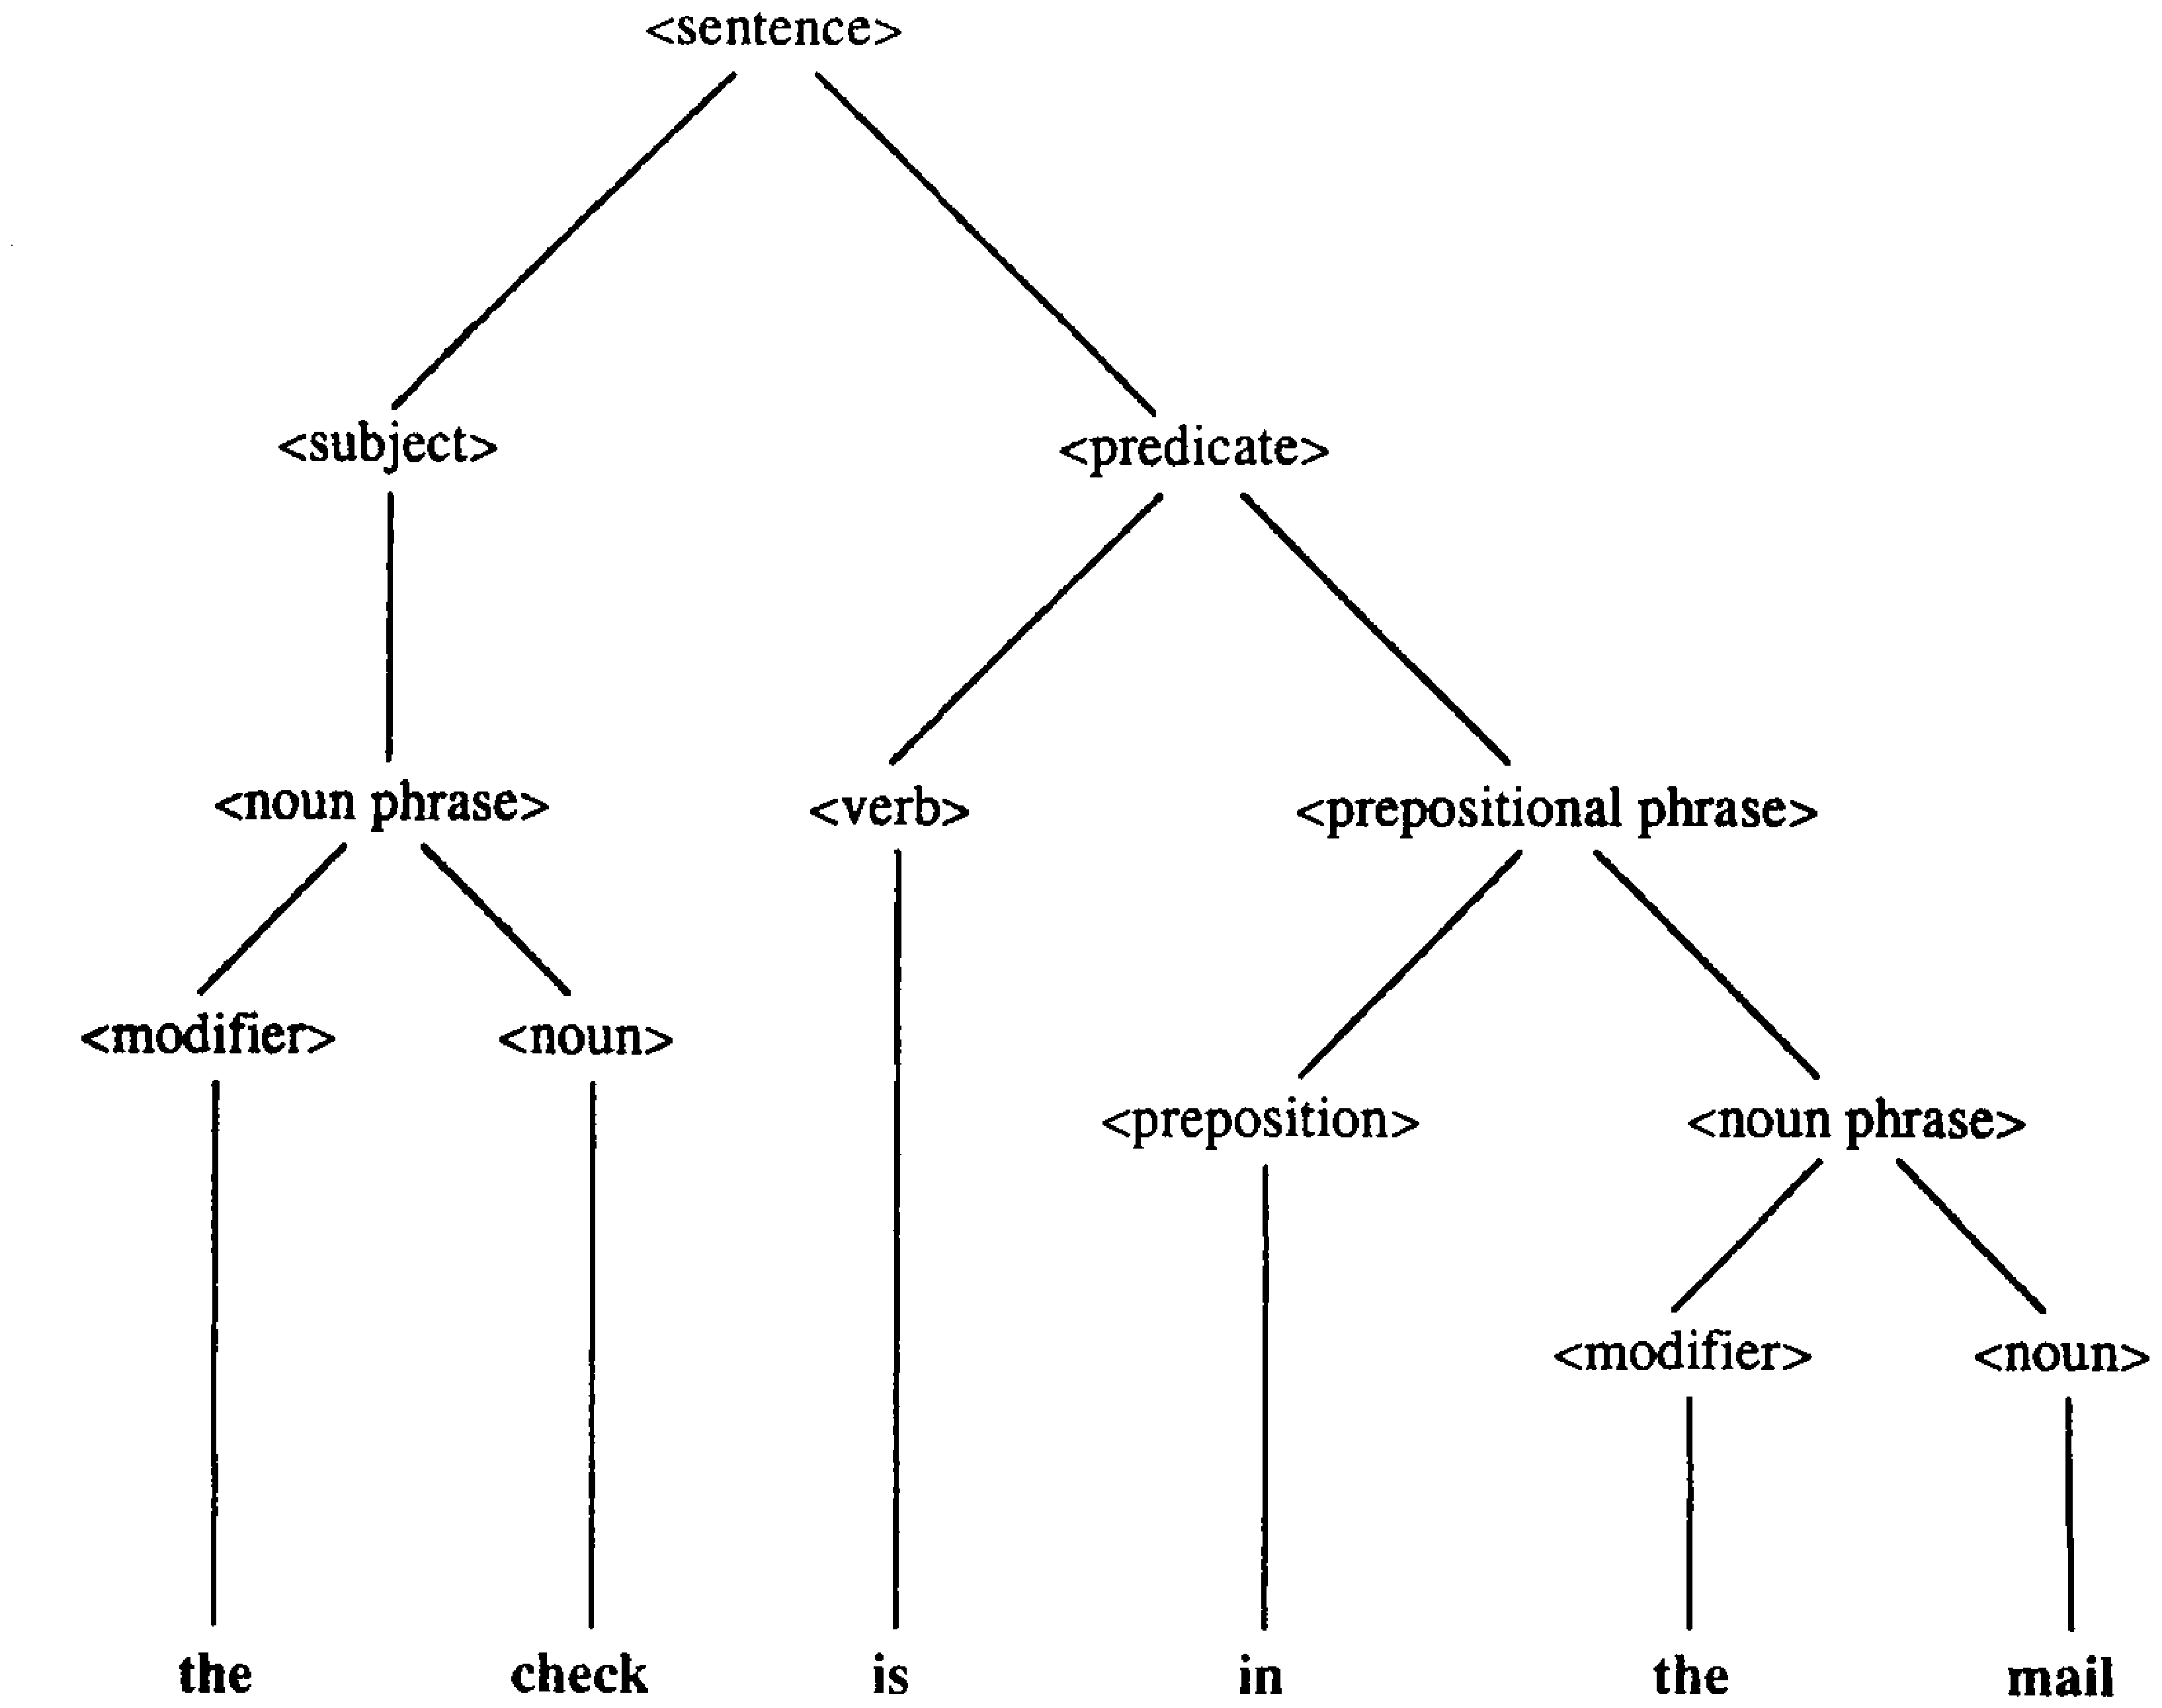
\epsfig{figure=ToFAfigures/fig9-1.eps,width=5.5in}}
\caption{A parse tree for the English grammar}\label{fig-9.1}
\end{figure}

\subsection*{Example 9.2}

Regular grammars form parse trees that are much more restrictive; at any given
level in the tree, only one node can be labeled with a nonterminal. Figure \ref{fig-9.2}
shows the parse tree for the word $\pmb{aaabaa}$ from the grammar
\[ G_1 = \langle\{T,S\},\{\pmb{a},\pmb{b}\},S,\{S\rightarrow\pmb{a}S,S
	\rightarrow\pmb{b}T,T\rightarrow\pmb{aa}\}\rangle. \]
In general, since productions in a right-linear grammar allow only the rightmost
symbol to be a nonterminal, parse trees for right-linear grammars will only
allow the rightmost child of a node to have a nontrivial subtree.

\subsection*{Example 9.3}\index{regular expression grammar}

Given a context-free grammar $G$, a common task required of compilers is to scan
a proposed terminal string $x$ belonging to $L(G)$ and build a parse tree
corresponding to $x$. If $G$ is the ``regular expression'' grammar defined in
Example 8.2, $G=\langle\{R\},\{\pmb{a},\pmb{b},\pmb{c},\pmb{(},\pmb{)},
\pmb{\epsilon},\pmb{\emptyset},\pmb{\cup},\pmb{\cdot},\pmb{^*}\},R,\{R
\rightarrow\pmb{a}|\pmb{b}|\pmb{c}|\pmb{\epsilon}|\pmb{\emptyset}|\pmb{(}R\pmb{\cdot} R\pmb{)}|\pmb{(}R
\pmb{\cup} R\pmb{)}|R\pmb{^*}\}\rangle$ and $x$ is $\pmb{((a\cup b)^*\!\!\cdot c)}$, the
desired result would be a representation of the tree shown in Figure \ref{fig-9.3}.

% Figure 9.2
\begin{figure}
\centerline{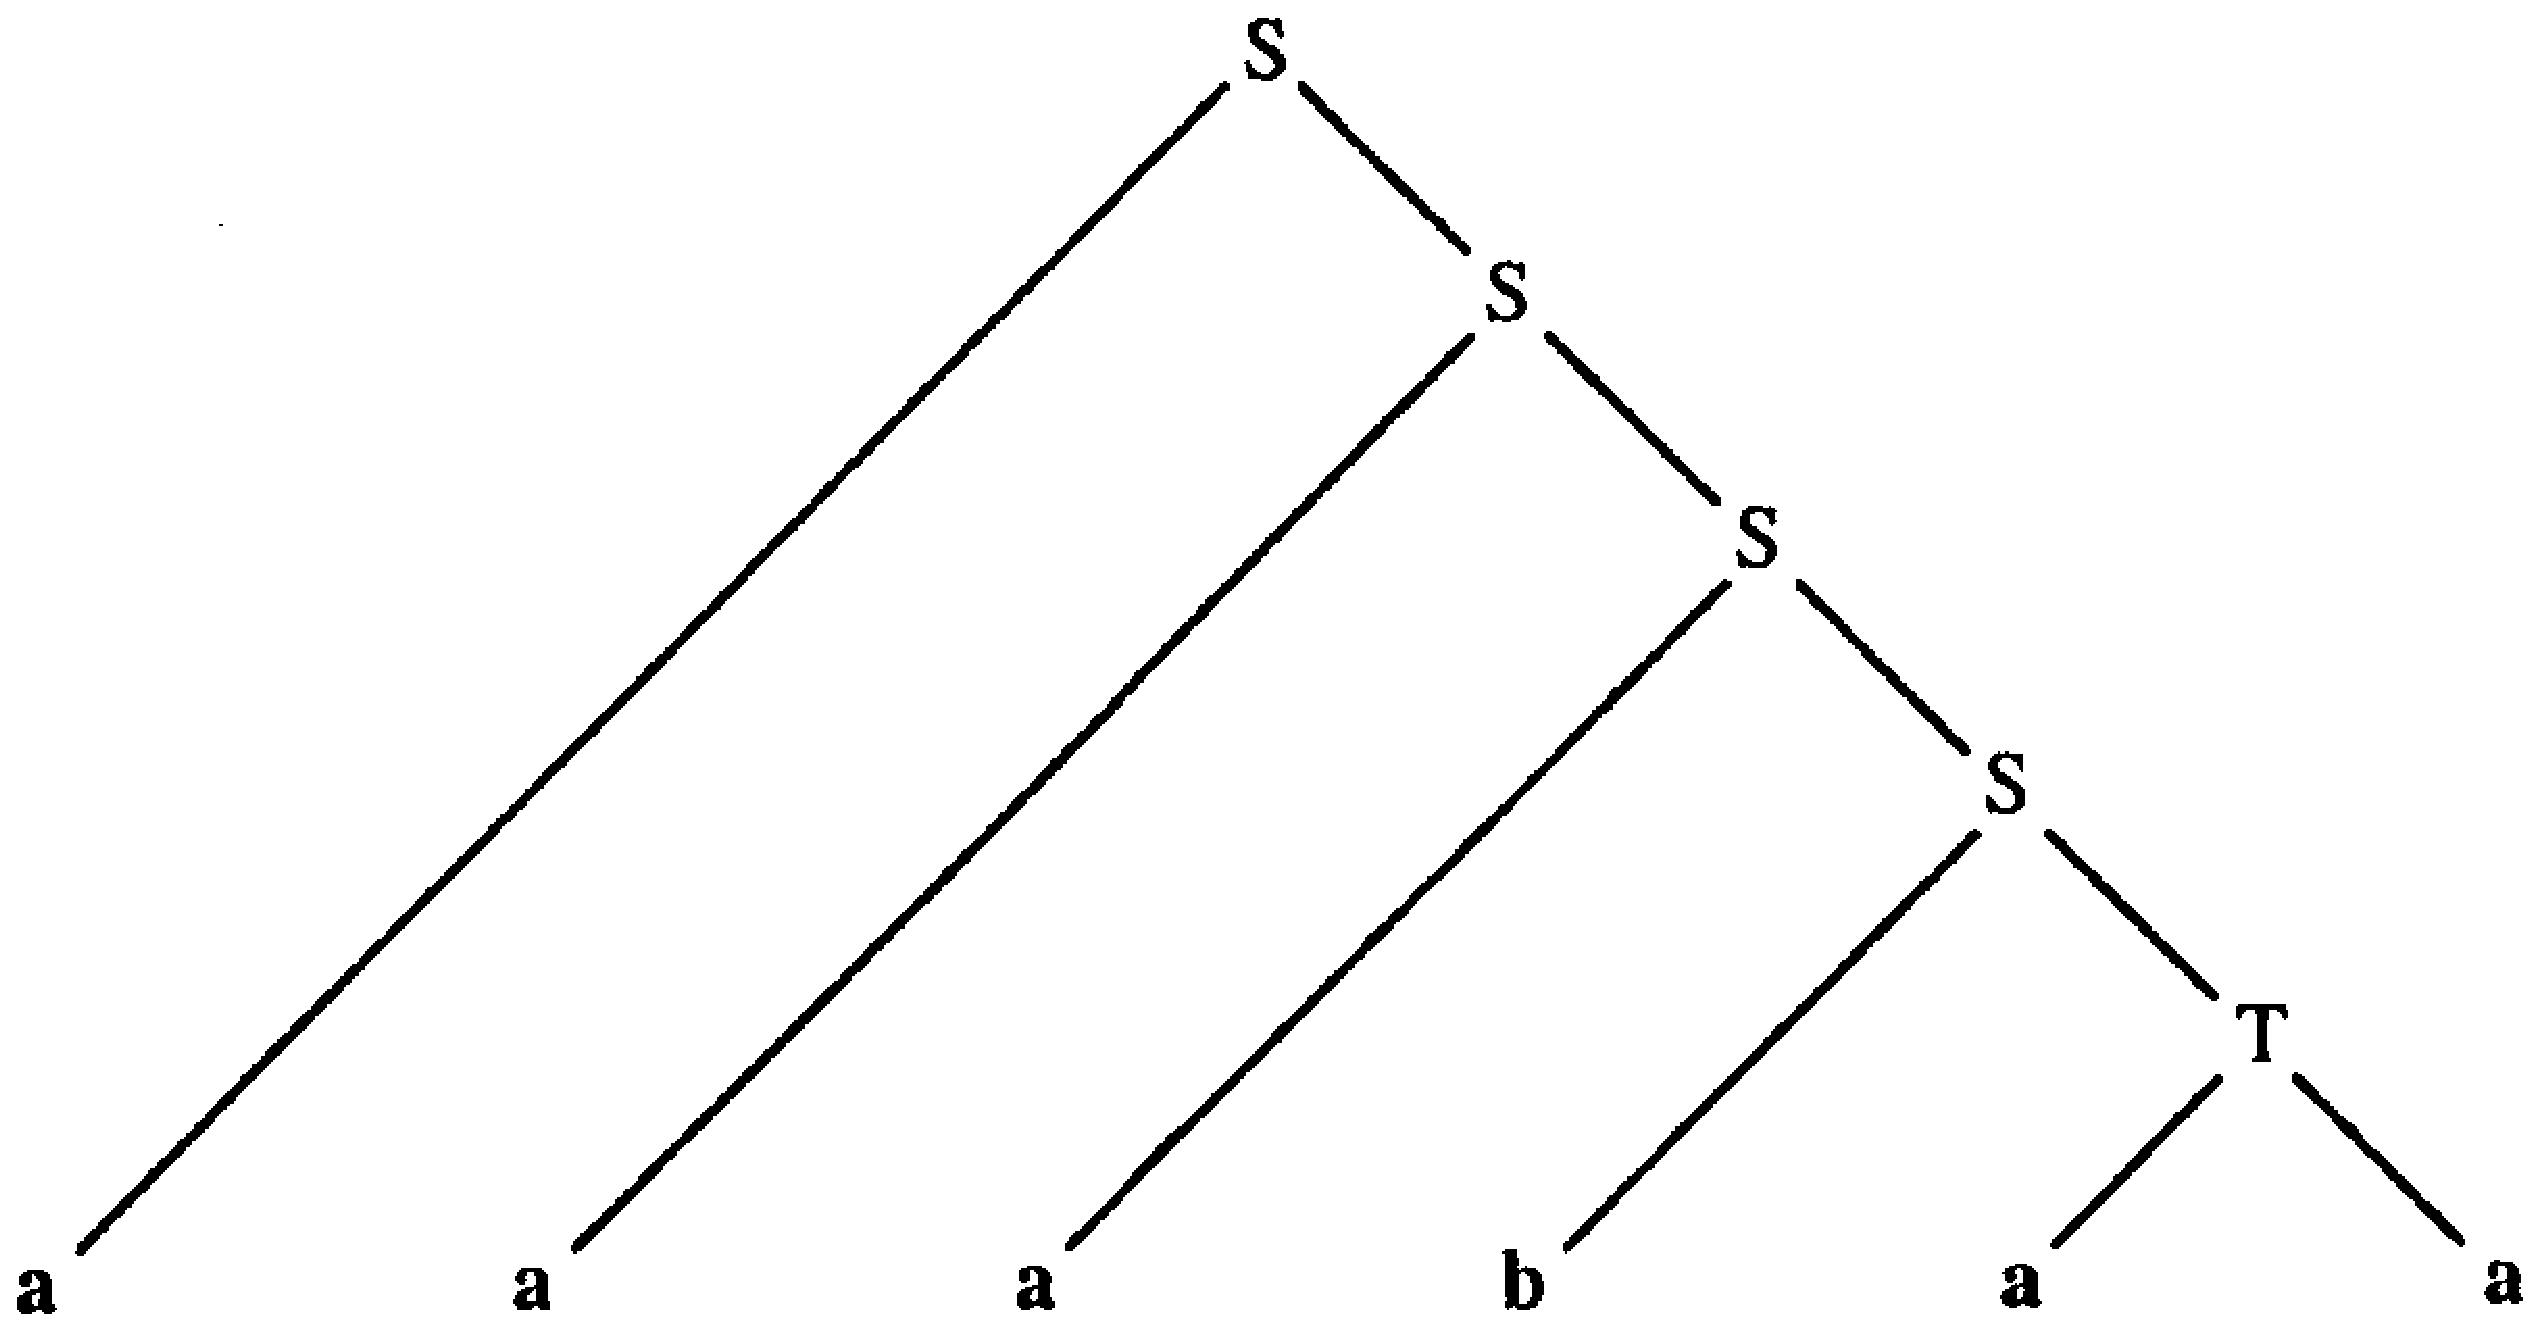
\epsfig{figure=ToFAfigures/fig9-2.eps,width=4.5in}}
\caption{The parse tree discussed in Example 9.2}\label{fig-9.2}
\end{figure}

In a perfect world of perfect programmers, it might be appropriate to assume
that $x$ can definitely be generated by the productions in $G$. In our world,
however, compilers must unfortunately perform the added task of determining
whether it is possible to generate the proposed terminal string $x$, that is,
whether the file presented represents a syntactically correct program. This is
typically done as the parse trees are being built, and discrepancies are
reported to the user. For the ``regular expression'' grammar used in Example
9.3, there is an algorithm for scanning the symbols of proposed strings such as
$\pmb{((a\cup b)^*\!\!\cdot c)}$ to determine whether a parse tree can be
constructed. In the case of a string like $\pmb{((a\cup b)}$, no such parse
tree exists, and the string therefore cannot be generated by the grammar. If the
productions of a grammar follow certain guidelines, the task of finding the
correct scanning algorithm is greatly simplified. The desired properties that
should be inherent in a programming language grammar are investigated later in
the text.

In a separate phase, after the parse trees are found, the compiler then uses
the trees and other constructs to infer meaning to the program, that is, to
generate appropriate machine code that reflects the advertised meaning (that is,
the \Index{semantics}) of the program statements. For example, the parse tree for
$((\pmb{a}\cup\pmb{b})^*\cdot\pmb{c})$ in Figure \ref{fig-9.3} clearly shows both the
order in which the operators $\cup$, $\cdot$, and $^*$ should be applied and the
expressions to which they should be applied.

Given a particular complete parse tree for a string $x$, there may be some
freedom in the order in which the associated productions are applied.

% Figure 9.3
\begin{figure}
\centerline{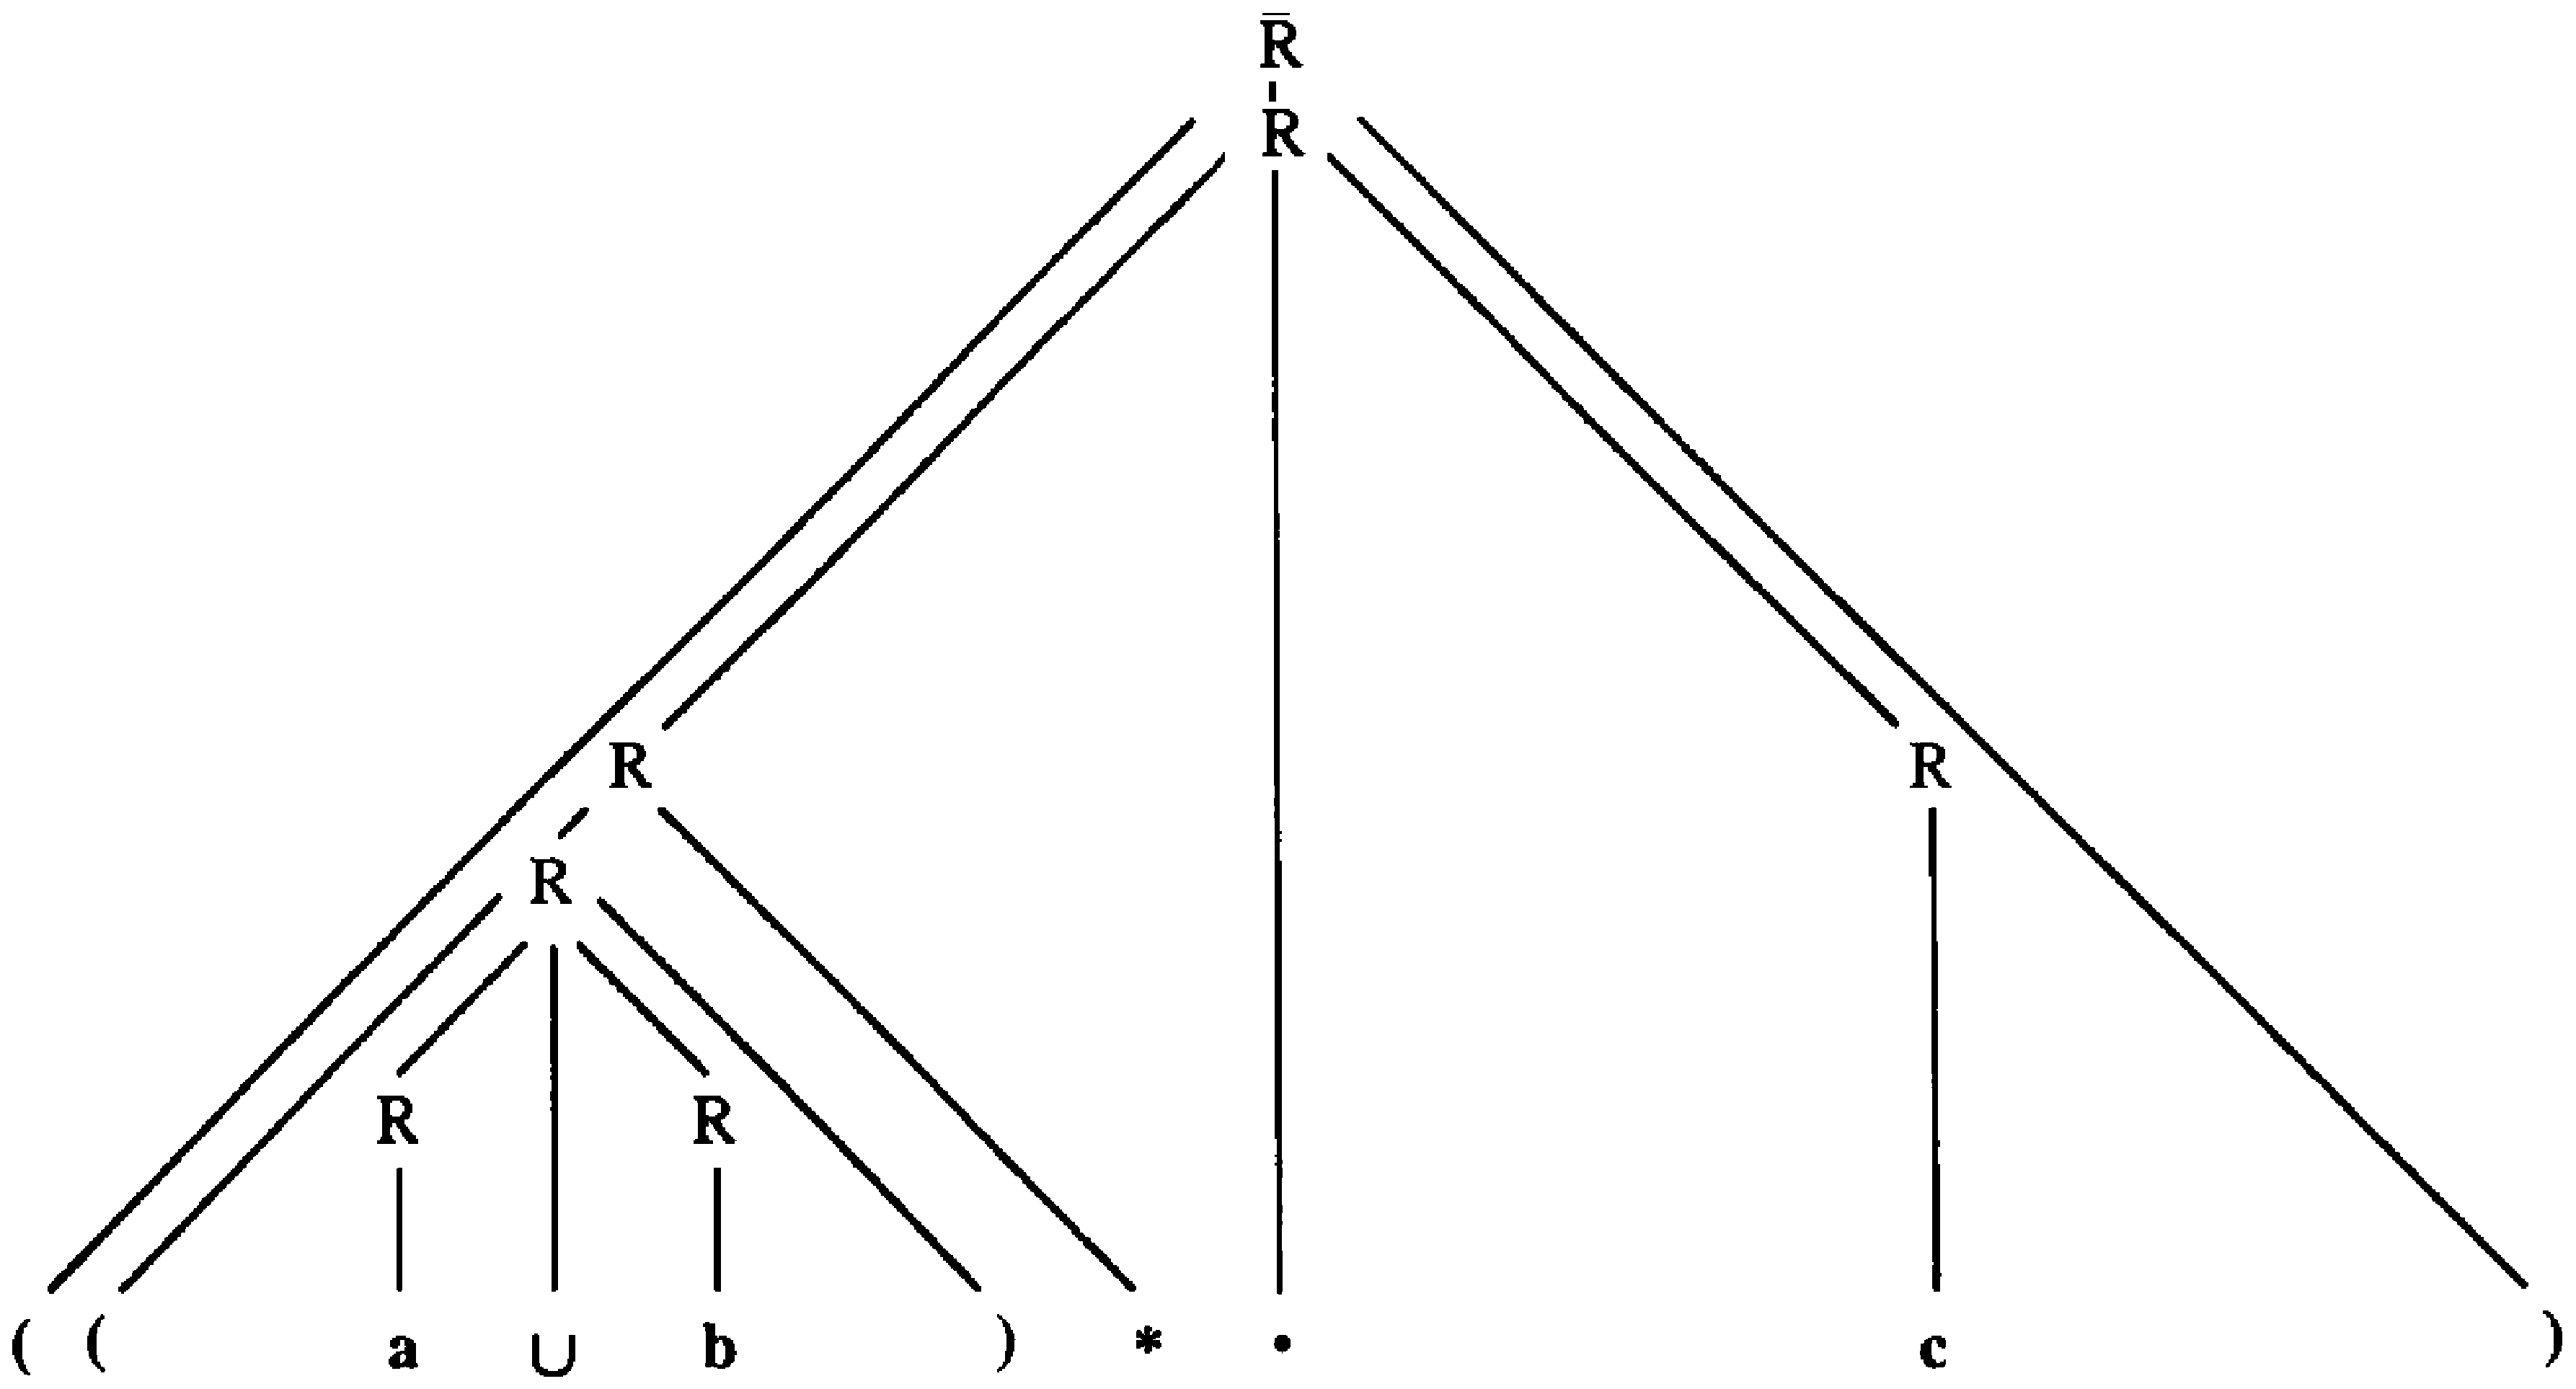
\epsfig{figure=ToFAfigures/fig9-3.eps,width=6.0in}}
\caption{The parse tree discussed in Example 9.3}\label{fig-9.3}
\end{figure}

\subsection*{Example 9.4}

For the grammar
\[ G=\langle\{R\},\{\pmb{a},\pmb{b},\pmb{c},\pmb{(},\pmb{)},
\pmb{\epsilon},\pmb{\emptyset},\pmb{\cup},\pmb{\cdot},\pmb{^*}\},R,\{R
\rightarrow\pmb{a}|\pmb{b}|\pmb{c}|\pmb{\epsilon}|\pmb{\emptyset}|
\pmb{(}R\pmb{\cdot} R\pmb{)}|\pmb{(}R\pmb{\cup} R\pmb{)}|R\pmb{^*}\}\rangle \]
%\[ G=\langle\{R\},\{\pmb{a},\pmb{b},\pmb{c},\pmb{(},\pmb{)},\pmb{\epsilon},
%	\pmb{\emptyset},\pmb{\cup},\pmb{\cdot},\pmb{^*}\},R,\{R\rightarrow
%	\pmb{a}|\pmb{b}|\pmb{c}|\pmb{\epsilon}|\pmb{\emptyset}|(R\cdot R)|(R\cup
%	R)|R^*\} \]
each of the following are valid derivations of the string $x=\pmb{((a\cup b)^*\!\!\cdot c)}$.

\noindent\emph{Derivation 1:}
\begin{center}\begin{tabular}{r@{ $\Rightarrow$ }l}
$R$ & $(R\cdot R)$ \\
& $(R^*\cdot R)$ \\
& $((R\cup R)^*\cdot R)$ \\
& $((\pmb{a}\cup R)^*\cdot R)$ \\
& $((\pmb{a}\cup\pmb{b})^*\cdot R)$ \\
& $((\pmb{a}\cup\pmb{b})^*\cdot\pmb{c})$
\end{tabular}\end{center}
\emph{Derivation 2:}
\begin{center}\begin{tabular}{r@{ $\Rightarrow$ }l}
$R$ & $(R\cdot R)$ \\
& $(R^*\cdot R)$ \\
& $((R\cup R)^*\cdot R)$ \\
& $((R\cup R)^*\cdot\pmb{c})$ \\
& $((R\cup\pmb{b})^*\cdot\pmb{c})$ \\
& $((\pmb{a}\cup\pmb{b})^*\cdot\pmb{c})$
\end{tabular}\end{center}
\emph{Derivation 3:}
\begin{center}\begin{tabular}{r@{ $\Rightarrow$ }l}
$R$ & $(R\cdot R)$ \\
& $(R\cdot\pmb{c})$ \\
& $(R^*\cdot\pmb{c})$ \\
& $((R\cup R)^*\cdot\pmb{c})$ \\
& $((\pmb{a}\cup R)^*\cdot\pmb{c})$ \\
& $((\pmb{a}\cup\pmb{b})^*\cdot\pmb{c})$
\end{tabular}\end{center}
\emph{Derivation 4:}
\begin{center}\begin{tabular}{r@{ $\Rightarrow$ }l}
$R$ & $(R\cdot R)$ \\
& $(R\cdot\pmb{c})$ \\
& $(R^*\cdot\pmb{c})$ \\
& $((R\cup R)^*\cdot\pmb{c})$ \\
& $((R\cup\pmb{b})^*\cdot\pmb{c})$ \\
& $((\pmb{a}\cup\pmb{b})^*\cdot\pmb{c})$
\end{tabular}\end{center}

% Definition 9.3
\begin{dfn}\label{dfn-9.3}\index{leftmost derivation}\index{rightmost derivation}
A derivation sequence is called a \emph{leftmost} derivation if at each
step in the sequence the leftmost nonterminal is next expanded to produce the
following step. A derivation sequence is called a \emph{rightmost}
derivation if at each step in the sequence the rightmost nonterminal is next
expanded to produce the following step.
\end{dfn}

The first of the derivations given in Example 9.4 is a \emph{leftmost}
derivation since at each step it is always the leftmost nonterminal that is
expanded to arrive at the next step. Similarly, the last of these, derivation
4, is a \emph{rightmost} derivation. There are many other possible derivations,
such as derivations 2 and 3, which are neither leftmost nor rightmost.

The restrictions on regular grammars ensure that there is never more than one
nonterminal present at any point during a derivation. This \emph{linear} nature
of regular grammars ensures that all derivations of a parse tree follow exactly
the same sequence, since there is never a choice of nonterrninals to expand.
Thus, the rightmost derivation of a parse tree in a regular grammar is always
the same as its leftmost derivation.

Parse trees in context-free grammars are generally more robust, allowing
several different derivation sequences to correspond to the same tree. For a
given parse tree, though, there is only one leftmost derivation. In Figure \ref{fig-9.4},
the nodes in the parse tree for $((\pmb{a}\cup\pmb{b})^*\!\cdot\pmb{c})$ are
numbered to show the order in which they would be visited by a \Index{preorder traversal}.
Note that the sequence in which the \emph{non}terminals would be
expanded in a leftmost derivation corresponds to the order in which they appear
in the preorder traversal.

% Figure 9.4
\begin{figure}
\centerline{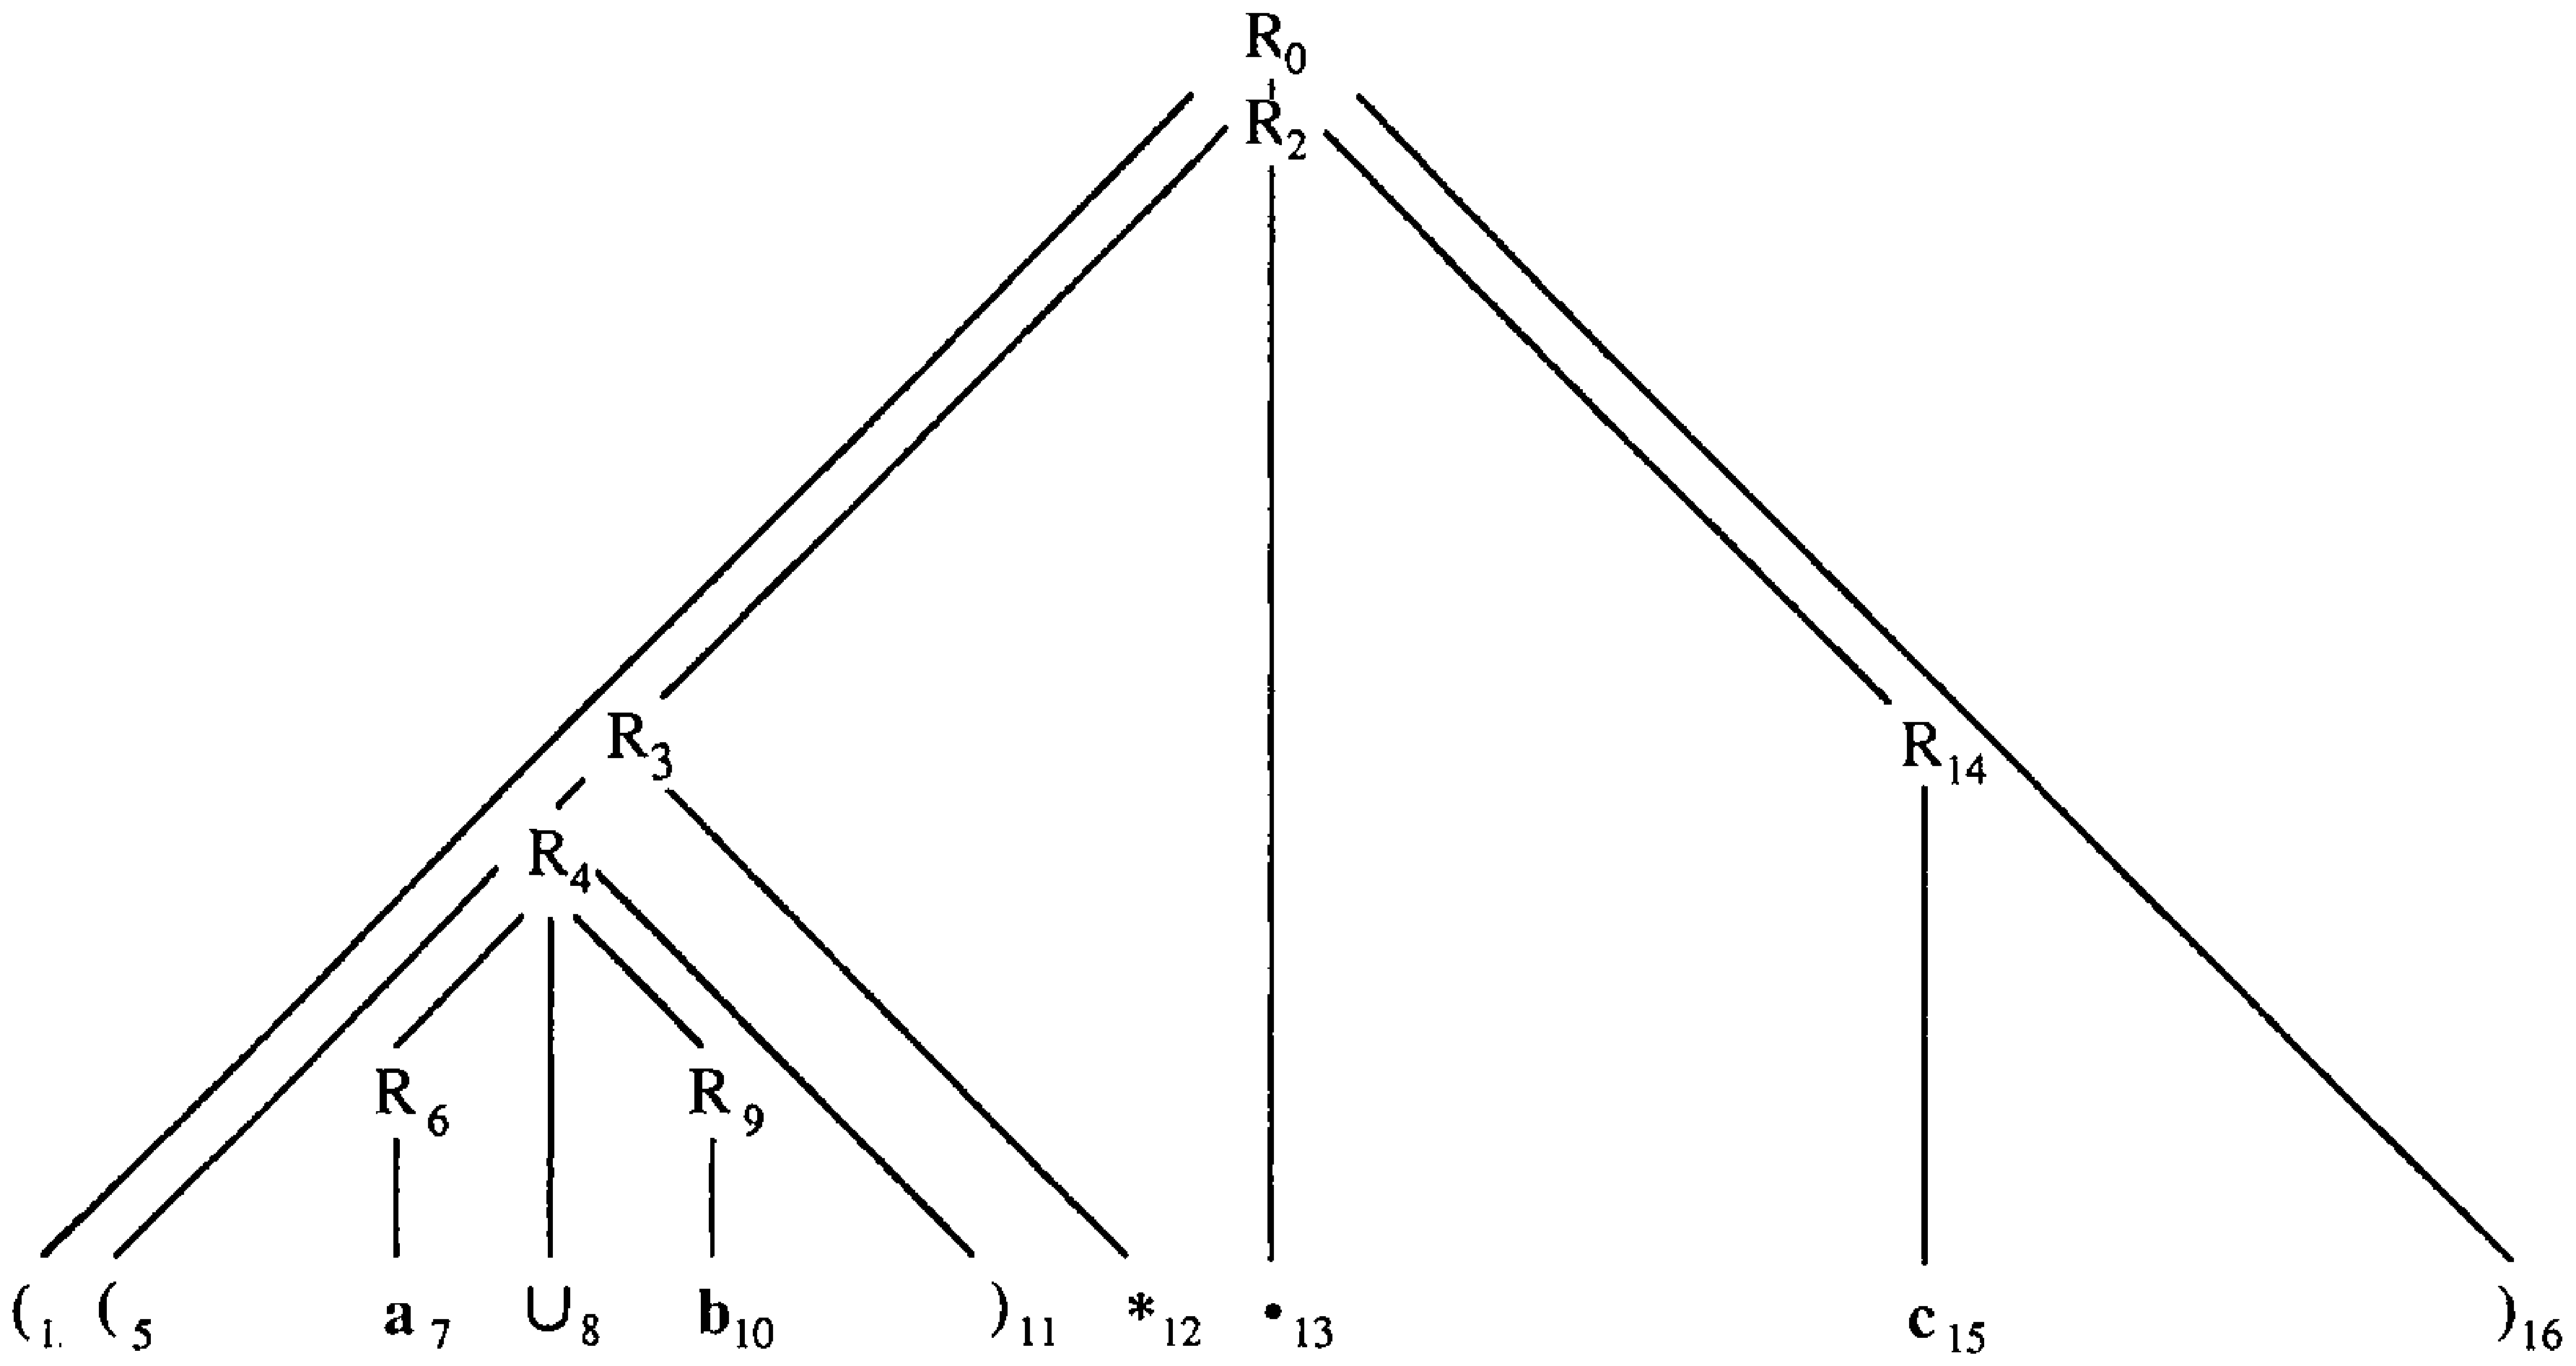
\epsfig{figure=ToFAfigures/fig9-4.eps,width=6.0in}}
\caption{The preorder traversal of the parse tree}\label{fig-9.4}
\end{figure}

\section{Ambiguity}\label{sec-9.2}

Whereas each tree corresponds to a unique leftmost derivation, it is possible
for a terminal string to have more than one leftmost derivation. This will
happen whenever a string $x$ corresponds to more than one parse tree, that is,
whenever there are truly distinct ways of applying the productions of the
grammar to form $x$. Grammars for which this can happen are called
\emph{ambiguous}.

% Definition 9.4
\begin{dfn}\label{dfn-9.4}\index{ambiguous context free grammar}\index{unambiguous grammar}
A grammar $G=\langle\Omega,\Sigma,S,P\rangle$ is called \emph{ambiguous}
if there exists a string $x\in\Sigma^*$ that corresponds to two distinct parse
trees. A grammar that is not ambiguous is called \emph{unambiguous}.
\end{dfn}

\subsection*{Example 9.5}

Consider the grammar $G_2=\langle\{S,A\},\{\pmb{a}\},S,\{S\rightarrow AA,A
\rightarrow\pmb{a}S\pmb{a},A\rightarrow\pmb{a}\}\rangle$. Figure \ref{fig-9.5} shows the
two distinct parse trees associated with the word $\pmb{aaaaa}$. Note that the
leftmost derivations corresponding to these trees are indeed different:
\begin{center}\begin{tabular}{r@{ $\Rightarrow$ }l}
$S$ & $AA$ \\
& $\pmb{a}S\pmb{a}A$ \\
& $\pmb{a}AA\pmb{a}A$ \\
& $\pmb{aa}A\pmb{a}A$ \\
& $\pmb{aaaa}A$ \\
& $\pmb{aaaaa}$
\end{tabular}\end{center}
is the sequence indicated by the parse tree in Figure \ref{fig-9.5}a, while
\begin{center}\begin{tabular}{r@{ $\Rightarrow$ }l}
$S$ & $AA$ \\
& $\pmb{a}A$ \\
& $\pmb{aa}S\pmb{a}$ \\
& $\pmb{aa}AA\pmb{a}$ \\
& $\pmb{aaa}A\pmb{a}$ \\
& $\pmb{aaaaa}$
\end{tabular}\end{center}
corresponds to Figure \ref{fig-9.5}b.

Recall that context-free grammars are used to inspect statements within a
computer program and determine corresponding parse trees. Such ambiguity is
undesirable in a grammar that describes a programming language, since it would
be unclear which of the trees should be used to infer the meaning of the string.
Indeed, this ambiguity would be intolerable if a statement could give rise to
two trees that implied different meanings, as illustrated in Example 9.6 below.
It is therefore of practical importance to avoid descriptions of languages that
entail this sort of ambiguity.

The language defined by the grammar $G_2$ in Example 9.5 is actually quite
simple. Even though $G_2$ is not a regular grammar, it can easily be shown that
$L(G_2)$ is the regular set $\{\pmb{a}^2,\pmb{a}^5,\pmb{a}^8,\pmb{a}^{11},
\pmb{a}^{14},\ldots\}$. The ambiguity is therefore not inherent in the language,
but is rather a consequence of the needlessly complex grammar used to describe
the language. A much simpler context-free grammar is given by $G_3=\langle\{T\},
\{\pmb{a}\},T,\{T\rightarrow\pmb{aaa}T,T\rightarrow\pmb{aa}\}\rangle$. This
grammar happens to be right linear and is definitely not ambiguous.

\subsection*{Example 9.6}\index{subtraction grammar}

% Figure 9.5
\begin{figure}
\centerline{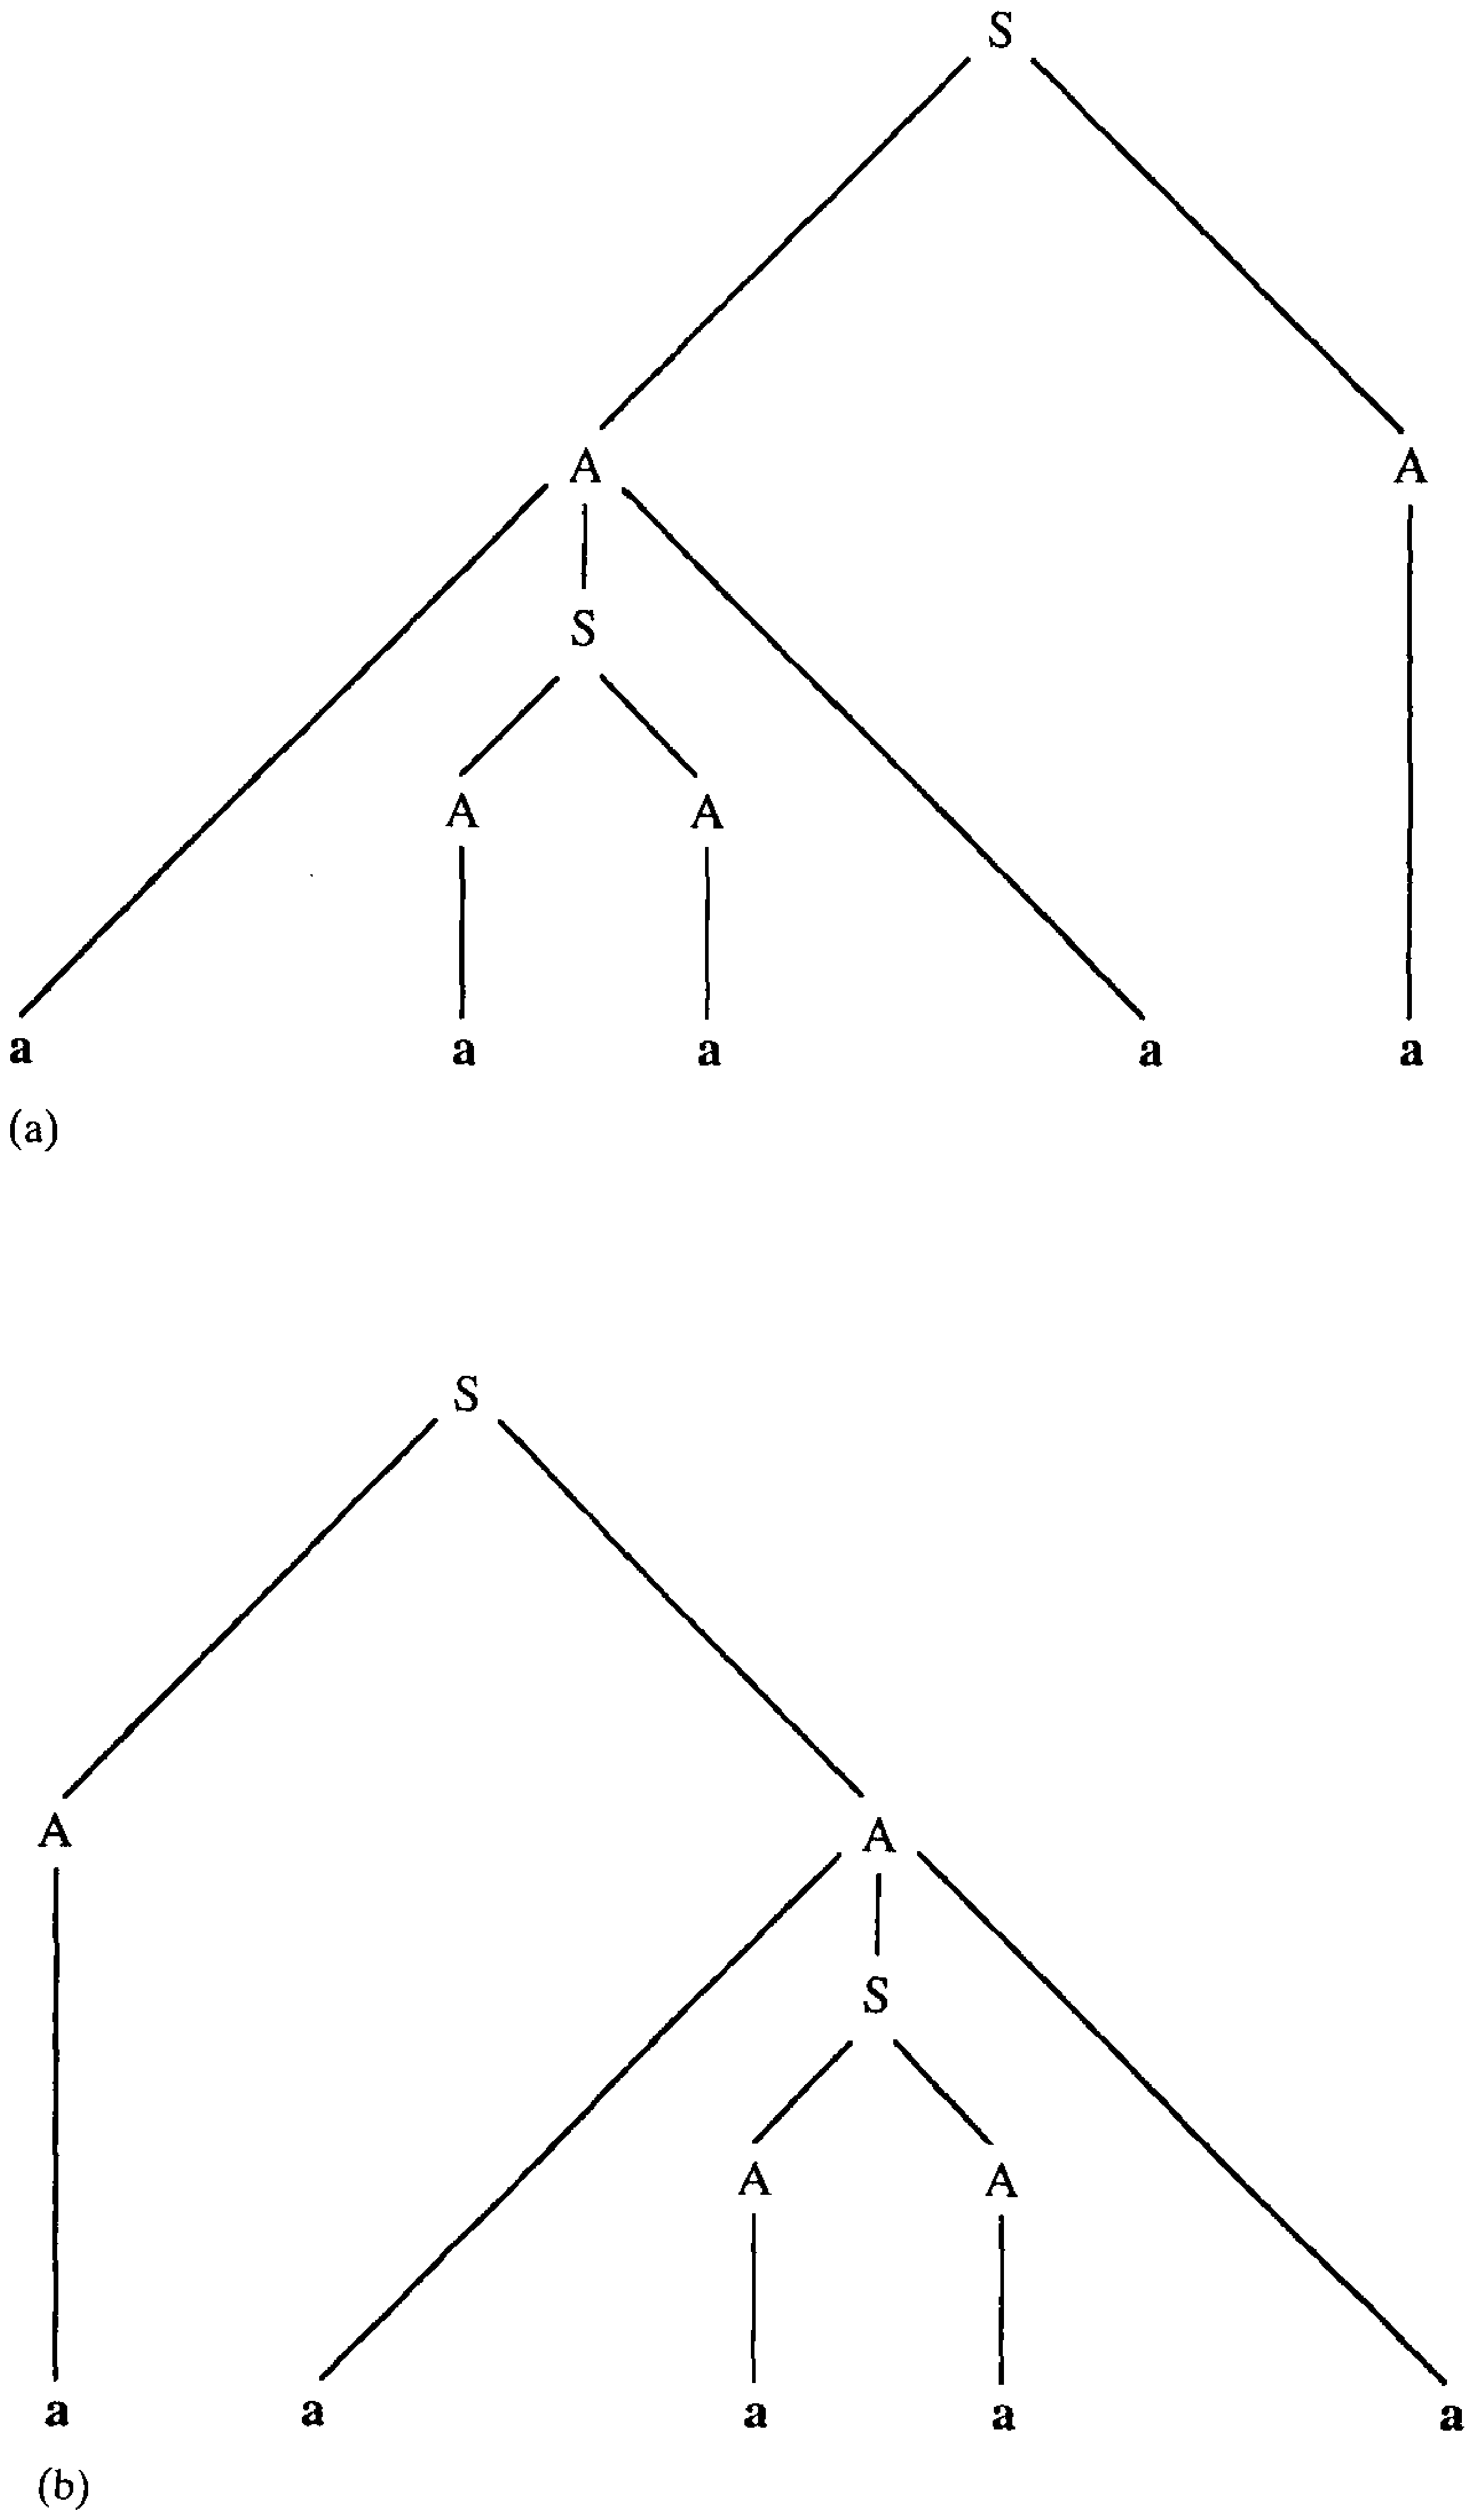
\epsfig{figure=ToFAfigures/fig9-5.eps,height=5.5in}}
\caption{(a) A parse tree for $\bf{aaaaa}$ in Example 9.5 (b) An alternate parse tree
for $\pmb{aaaaa}$}\label{fig-9.5}
\end{figure}

The following sampling from a potential programming language grammar illustrates
the semantic problems that can be caused by ambiguity. Consider the grammar
$G_s=\langle\{<$expression$>,<$identifier$>\},\{\pmb{a},\pmb{b},\\\pmb{c},\pmb{d},
\pmb{-}\},<$expression$>,P\rangle$, where $P$ consists of the productions
\begin{center}\begin{tabular}{r@{ $\rightarrow$ }l}
\<expression\> & \<identifier\> \\
\<expression\> & \<identifier\> -- \<expression\> \\
\<expression\> & \<expression\> -- \<identifier\> \\
\<identifier\> & $\pmb{a}$ \\
\<identifier\> & $\pmb{b}$ \\
\<identifier\> & $\pmb{c}$ \\
\<identifier\> & $\pmb{d}$
\end{tabular}\end{center}
$L(G_s)$ then contains the string $\pmb{a-b-d}$, which can be generated by
two distinct parse trees, as shown in Figure \ref{fig-9.6}. Figure \ref{fig-9.6}a corresponds to the
following leftmost derivation.
\begin{center}\begin{tabular}{r@{ $\Rightarrow$ }l}
\<expression\> & \<expression\> -- \<identifier\> \\
& \<identifier\> -- \<expression\> -- \<identifier> \\
& $\pmb{a-}$ \<expression\> -- \<identifier\> \\
& $\pmb{a-}$ \<identifier\> -- \<identifier\> \\
& $\pmb{a-b-}$ \<identifier\> \\
& $\pmb{a-b-d}$
\end{tabular}\end{center}
Figure \ref{fig-9.6}b corresponds to a different leftmost derivation, as shown below.
\begin{center}\begin{tabular}{r@{ $\Rightarrow$ }l}
\<expression\> & \<identifier\> -- \<expression\> \\
& $\pmb{a-}$ \<expression\> \\
& $\pmb{a-}$ \<identifier\> -- \<expression\> \\
& $\pmb{a-b-}$ \<expression\> \\
& $\pmb{a-b-}$ \<identifier\> \\
& $\pmb{a-b-d}$
\end{tabular}\end{center}
If the productions of $G_s$ were part of a grammatical description of a
programming language, there are obvious semantics associated with the
productions involving the $\pmb{-}$ operator. The productions
\[ \text{\<expression\>}\rightarrow\text{\<identifier\>}-\text{\<expression\>}\]
and
\[ \text{\<expression\>}\rightarrow\text{\<expression\>}-\text{\<identifier\>}\]
indicate that two values should be combined using the subtraction operator to
form a new value. The compiler would be responsible for generating code that
carried out the appropriate subtraction. Unfortunately, the two parse trees give
rise to functionally different code. For the parse tree in Figure \ref{fig-9.6}a, the
subtraction will be performed left to right, while in the parse tree in Figure
\ref{fig-9.6}b the ordering of the operators is right to left. Subtraction is \emph{not} a
commutative operation, and the expression $(a-b)-d$ will usually produce a
different value than $a-(b-d)$. Ambiguity can thus be a fatal flaw in a grammar
describing a programming language.

% Figure 9.6
\begin{figure}
\centerline{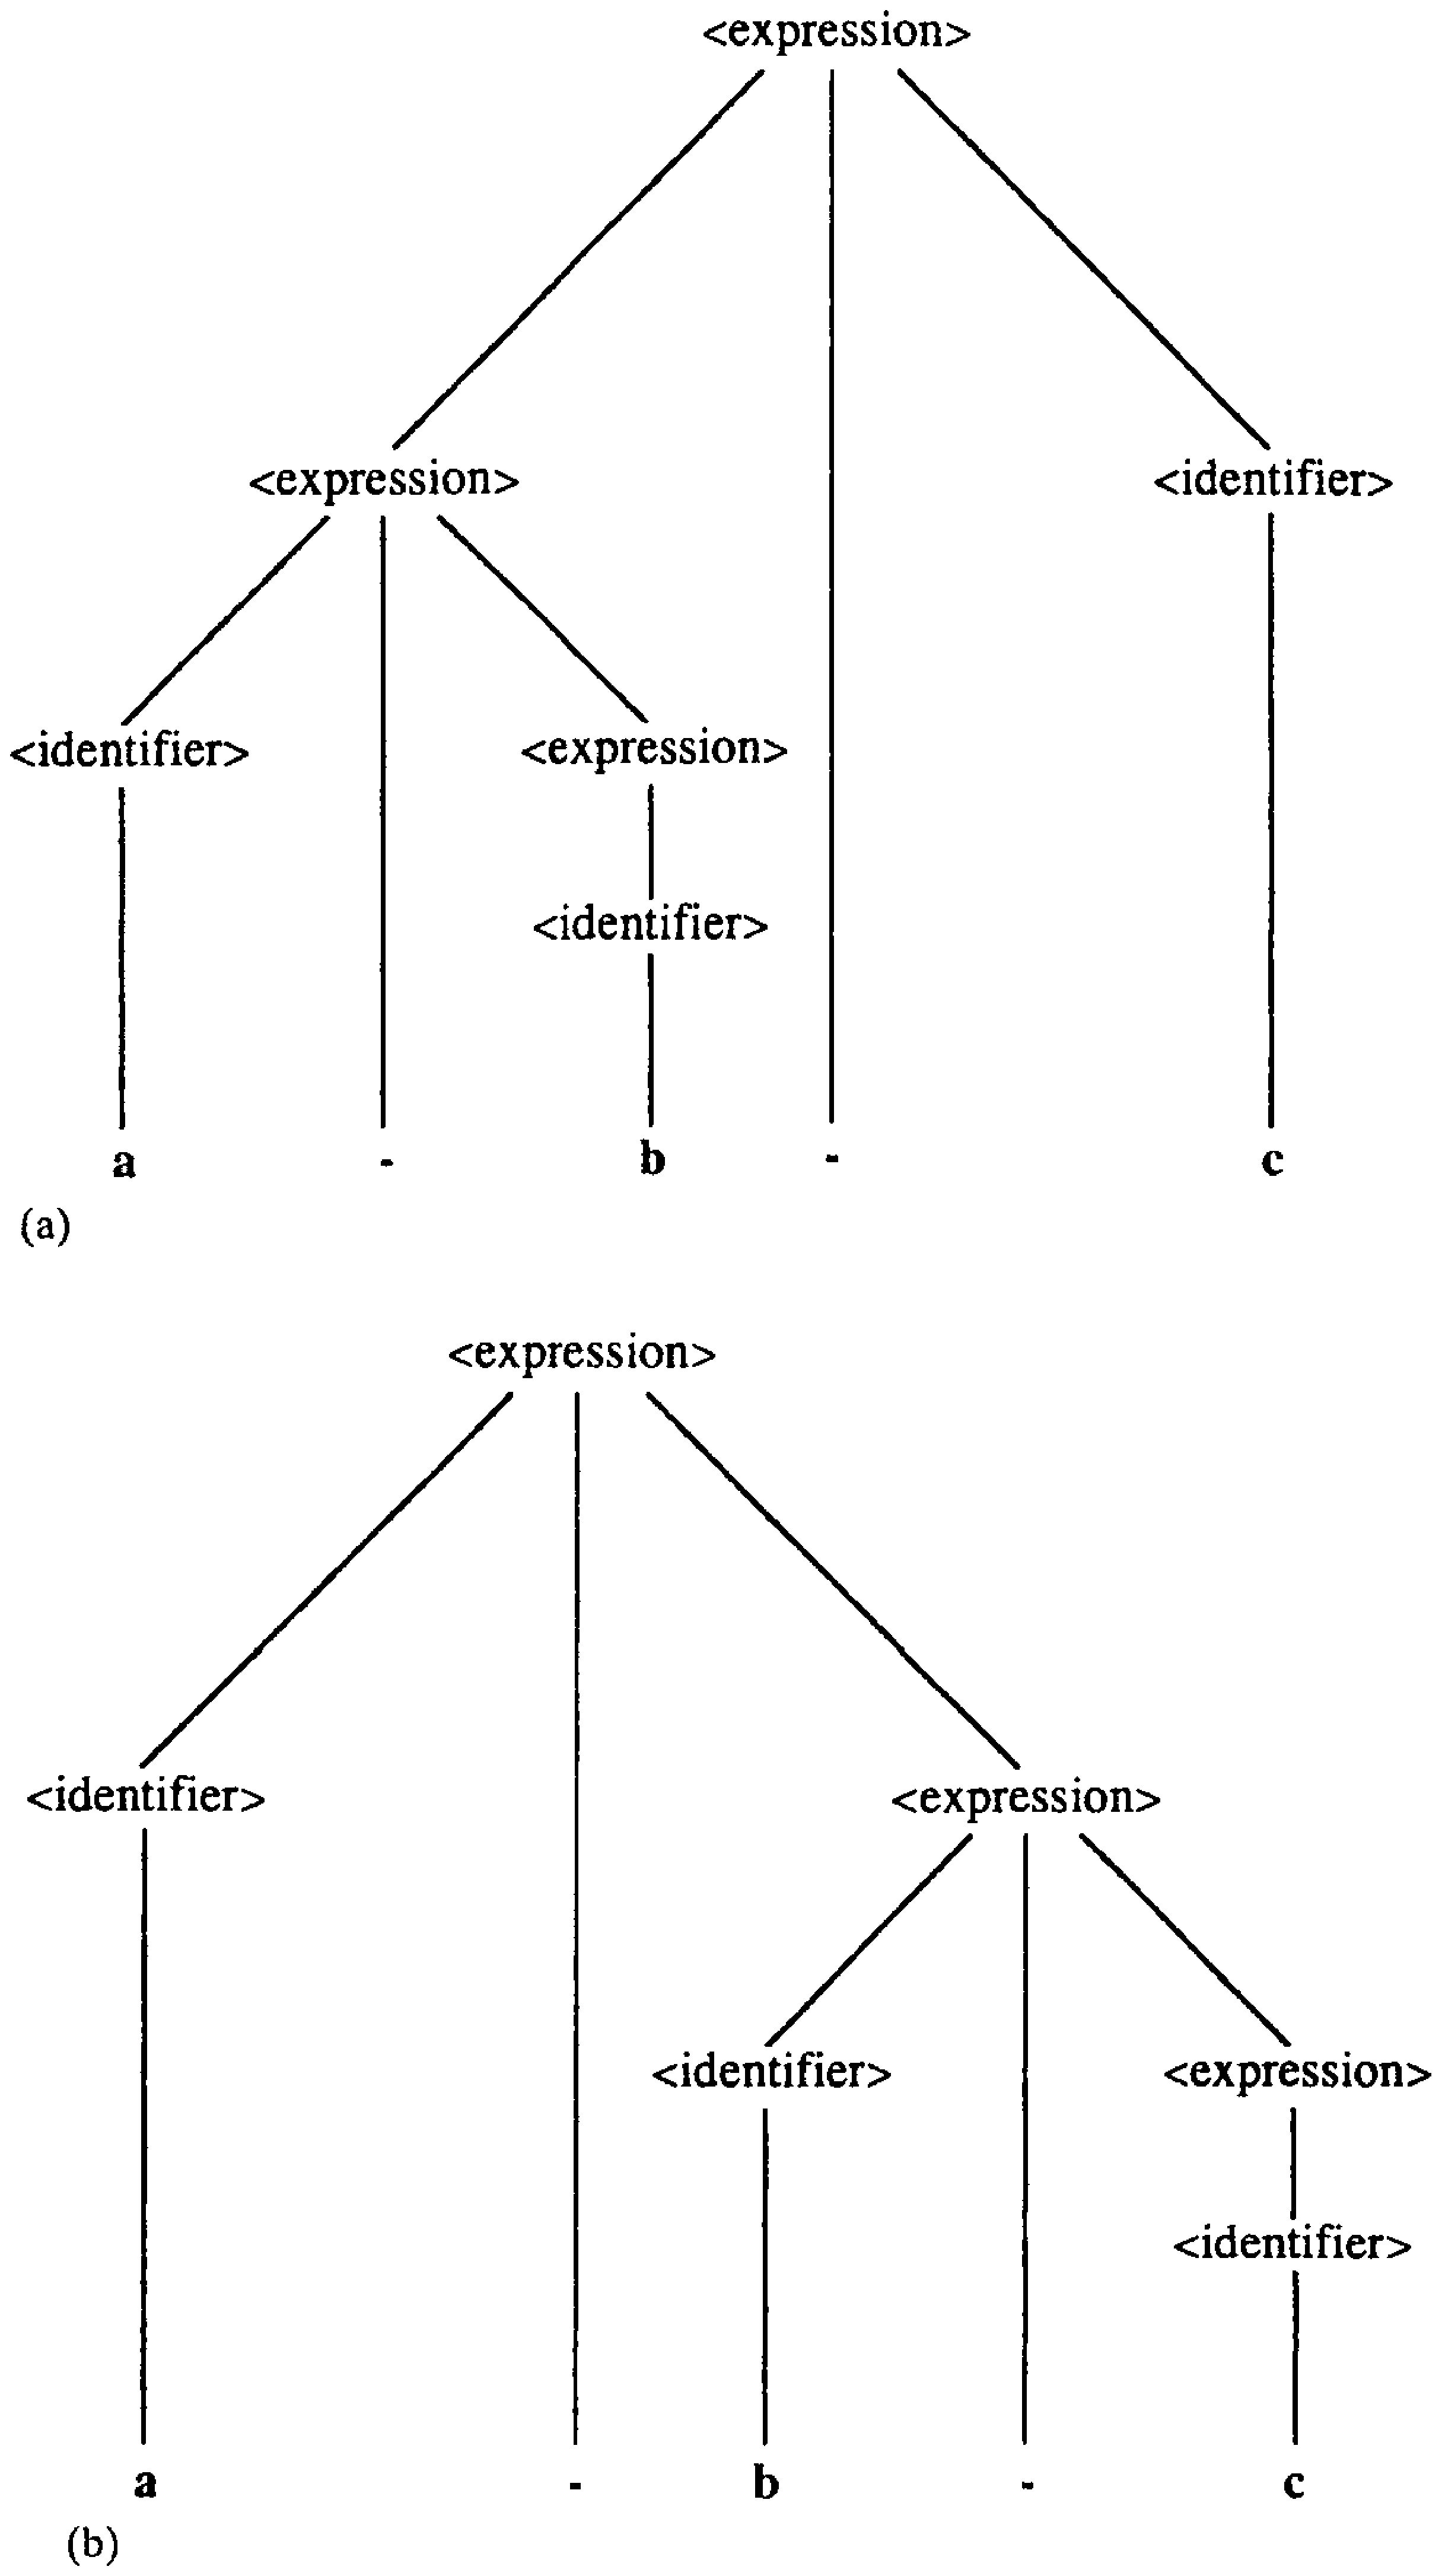
\epsfig{figure=ToFAfigures/fig9-6.eps,height=6.5in}}
\caption{(a) A parse tree for $\pmb{a-b-d}$ in Example 9.6 (b) An alternate
parse tree for $\pmb{a-b-d}$}\label{fig-9.6}
\end{figure}

In the language $L(G_s)$ discussed in Example 9.6, the ambiguity is again not
inherent in the language itself, but is rather a consequence of the specific
productions in the grammar $G_s$ describing the language. In most programming
languages, the expression $\pmb{a-b-d}$ is allowed and has a well-defined
meaning. Most languages decree that such expressions be evaluated from left to
right, and hence $\pmb{a-b-d}$ would be interpreted as ($\pmb{a-b}$)$\pmb{-d}$.
This interpretation can be enforced by simply removing the production
\[ \text{\<expression\>}\rightarrow\text{\<identifier\>}-\text{\<expression\>}\]
from $G_s$ to form the new grammar
\[ G_m = \langle\{\text{\<expression\>},\text{\<identifier\>}\},\{\pmb{a},\pmb{b},
	\pmb{c},\pmb{d},\pmb{-}\},\text{\<expression\>},P'\rangle \]
where $P'$ consists of the productions
\begin{center}\begin{tabular}{r@{ $\rightarrow$ }l}
\<expression\> & \<identifier\> \\
\<expression\> & \<expression\> -- \<identifier\> \\
\<identifier\> & $\pmb{a}$ \\
\<identifier\> & $\pmb{b}$ \\
\<identifier\> & $\pmb{c}$ \\
\<identifier\> & $\pmb{d}$
\end{tabular}\end{center}

It should be clear that $G_s$ and $G_m$ are equivalent, and both generate the
regular language $((\pmb{a}\cup\pmb{b}\cup\pmb{c}\cup\pmb{d})\cdot\pmb{-})^*
\cdot(\pmb{a}\cup\pmb{b}\cup\pmb{c}\cup\pmb{d})$. $G_m$ gives rise to unique
parse trees and is therefore unambiguous. It should be noted that the language
could have been defined with a single nonterminal; a simpler grammar equivalent
to $G_m$ is $G_t = \langle\{T\},\{\pmb{a},\pmb{b},\pmb{c},\pmb{d},\pmb{-}\},T,\{
T\rightarrow\pmb{a}|\pmb{b}|\pmb{c}|\pmb{d}|T - T\}\rangle$. However, since
$G_t$ is ambiguous, it is much more difficult to work with than $G_m$. The pair
of nonterminals \<expression\> and \<identifier\> are used to circumvent the
ambiguity problem in this language. For the grammar $G_m$, the production
\[ \text{\<expression\>}\rightarrow\text{\<expression\>}-\text{\<identifier\>}\]
contains the nonterminal \<expression\> to the left of the subtraction token and
\<identifier\> to the right of the $\pmb{-}$. Since \<identifier\> can only be
replaced by a terminal representing a single variable, the resulting parse tree
will ensure that the entire expression to the left of the $\pmb{-}$ will be
evaluated before the operation corresponding to this current subtraction token
is performed. In this fashion, the distinction between the two nonterminals
forces a left-to-right evaluation sequence. In fact, a more robust language with
other operators like $\times$ and $\div$ will require more nonterminals to
enforce the default precedence among these operators.

Most modern programming languages employ a solution to the ambiguity problem
that is different from the one just described. Programmers generally do not
want to be constrained by operators that can only be evaluated from left to
right, and hence matched parentheses are used to indicate an order of evaluation
that may differ from the default. Thus, unambiguous grammars that correctly
reflect the meaning of expressions like $d-(b-c)$ or even $(a)-((c-(d)))$ are
sought.

\subsection*{Example 9.7}

The following grammar $G_P$ allows expressions with parentheses, minus signs,
and single-letter identifiers to be uniquely parsed.
\[ G_P = \langle\{\text{\<expression\>},\text{\<identifier\>}\},\{\pmb{a},
	\pmb{b},\pmb{c},\pmb{d},\pmb{-},\pmb{(},\pmb{)}\},\text{\<expression\>},
	P''\rangle \]
where $P''$ consists of the productions
\begin{center}\begin{tabular}{r@{ $\rightarrow$ }l}
\<expression\> & (\<expression\>) \\
\<expression\> & \<expression\> -- (\<expression\>) \\
\<expression\> & \<identifier\> \\
\<expression\> & \<expression\> -- \<identifier\> \\
\<identifier\> & $\pmb{a}$ \\
\<identifier\> & $\pmb{b}$ \\
\<identifier\> & $\pmb{c}$ \\
\<identifier\> & $\pmb{d}$
\end{tabular}\end{center}

The first two productions in $P''$, which were not present in $P'$, are designed
to handle the balancing of parentheses. The first rule allows superfluous sets
of parentheses to be correctly recognized. The second rule ensures that an
expression that is surrounded by parentheses is evaluated before the operator
outside those parentheses is evaluated. In the absence of parentheses, the
left-to-right ordering of the operators is maintained. Figure \ref{fig-9.7} illustrates
the unique parse tree for the expression $(a)-((c-(d)))$.

$G_P$ is a context-free language that is too complex to be regular; the pumping
lemma for regular sets (Theorem \ref{thm-2.3}) can be used to show that is impossible for
a DFA to maintain an unlimited number of corresponding balanced parentheses.
This language, and the others discussed so far, can all be expressed by
unambiguous grammars. It should be clear that \emph{every} language generated by
grammars has ambiguous grammars that also generate it, since an unambiguous
grammar can always be modified to become ambiguous. What is not immediately
clear is whether there are languages that can \emph{only} be generated by
ambiguous grammars.

% Definition 9.5
\begin{dfn}\label{dfn-9.5}\index{unambiguous context free grammar}\index{inherently ambiguous}\index{language!inherently ambiguous}\index{language!unambiguous}
A context-free language $L$ is called \emph{inherently ambiguous} if
every grammar that generates $L$ is ambiguous. A context-free language that is
not inherently ambiguous is called \emph{unambiguous}.
\end{dfn}

% Definition 9.6
\begin{dfn}\label{dfn}\index{C@\CSIG \ (C-sigma)}\index{U@\USIG \ (U-sigma )}
Let the class of context-free language $L$ over the alphabet $\Sigma$ be denoted
by \CSIG. Let the class of unambiguous context-free languages be denoted by
\USIG
\end{dfn}

% Theorem 9.1
\begin{thm}\label{thm-9.1}\index{ambiguous context free language, inherently}\index{inherently ambiguous}
There are context-free languages that are inherently ambiguous; that is, \USIG\ 
is properly contained in \CSIG.

\emph{Proof.} The language $L=\{\pmb{a}^n\pmb{b}^n\pmb{c}^m\pmb{d}^m|n,m\in\NN\}
\cup\{\pmb{a}^i\pmb{b}^j\pmb{c}^j\pmb{d}^i|i,j\in\NN\}$ is a context-free
language (see the exercises). $L$ is also inherently ambiguous, since there must
exist two parse trees for some of the strings in the intersection of the two
sets $\{\pmb{a}^n\pmb{b}^n\pmb{c}^m\pmb{d}^m|n,m\in\NN\}$ and $\{\pmb{a}^i\pmb{b}
^j\pmb{c}^j\pmb{d}^i|i,j\in\NN\}$. The proof of this last statement is
tedious to formalize; the interested reader is referred to [HOPC].
\end{thm}

% Figure 9.7
\begin{figure}
\centerline{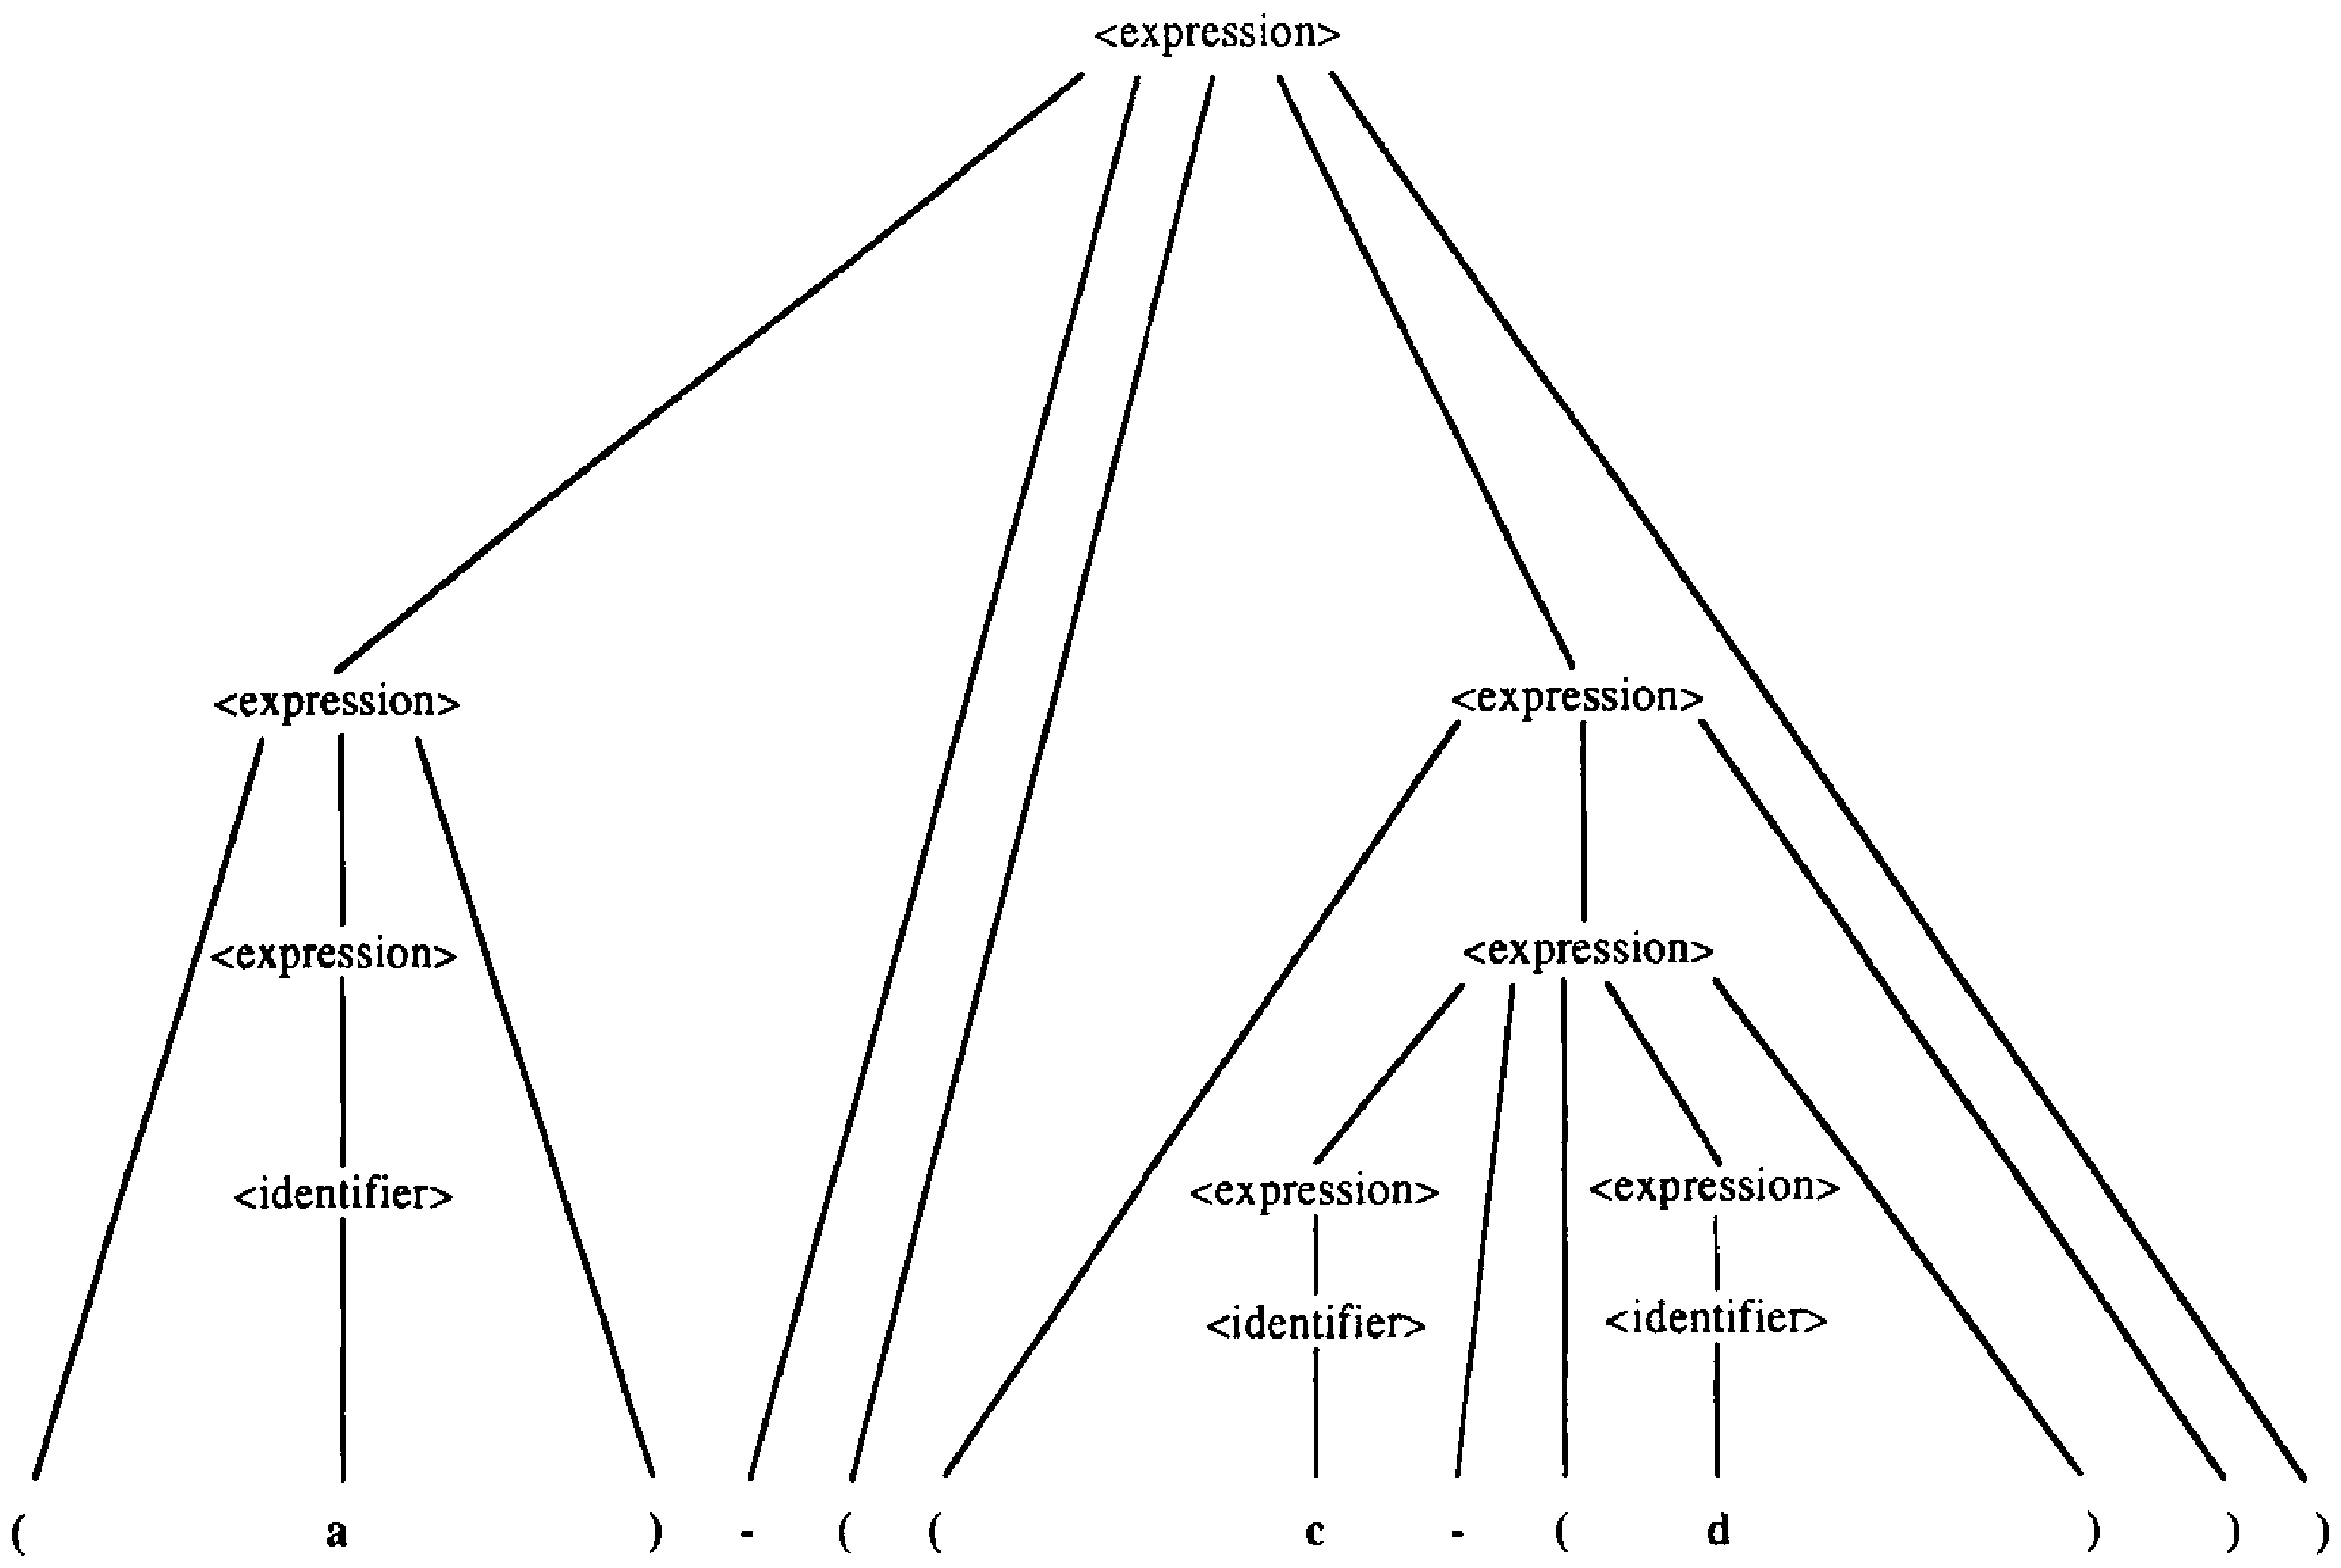
\epsfig{figure=ToFAfigures/fig9-7.eps,height=3.5in}}
\caption{The parse tree discussed in Example 9.7}\label{fig-9.7}
\end{figure}

Theorem \ref{thm-9.1} states that there exist inherently ambiguous type 2 languages. No
type 3 language is inherently ambiguous. Even though there are regular grammars
that are ambiguous, every regular grammar has an equivalent grammar that is
unambiguous. This assertion is supported by the following examples and
results.

\subsection*{Example 9.8}

Consider the following right-linear grammar $G_r$:
\[ G_r = \langle\{S,A,C\},\{\pmb{a},\pmb{b},\pmb{c}\},S,\{S\rightarrow A\pmb{bc},
	S\rightarrow\pmb{ab}C,A\rightarrow\pmb{a},C\rightarrow\pmb{c}\}\rangle \]
Only one terminal string can be derived from $G_r$, but this word has two
distinct derivation trees, as shown in Figure \ref{fig-9.8}. Thus, there are regular
grammars that are ambiguous.

% Theorem 9.2
\begin{thm}\label{thm-9.2}
Given any right-linear grammar\ \,$G=\langle\Omega,\Sigma,S,P\rangle$, there exists
an equivalent right-linear grammar that is unambiguous.

\emph{Proof.} Let $G'=G_{(A^{\sigma d}_G)}$. That is, beginning with the
right-linear grammar G, use the construction outlined in Lemma \ref{lmm-8.2} to find the
corresponding automaton $A_G$. Use Definition \ref{dfn-4.9} to remove the
lambda-transitions and Definition \ref{dfn-4.5} to produce a deterministic machine, and
then apply the construction outlined in Lemma \ref{lmm-8.1} to form the new right-linear
grammar $G'$. By Lemma \ref{lmm-8.2}, Theorem \ref{thm-4.2}, Theorem \ref{thm-4.1}, and Lemma \ref{lmm-8.1}, the
language defined by each of these constructs is unchanged, so $G'$ is equivalent
to $G$. Due to the deterministic nature of the machine from which this new
grammar was built, the resulting parse tree for a given string must be unique,
since only one production is applicable at any point in the derivation. A formal
inductive statement of this property is left as an exercise.
\end{thm}

% Figure 9.8
\begin{figure}
\centerline{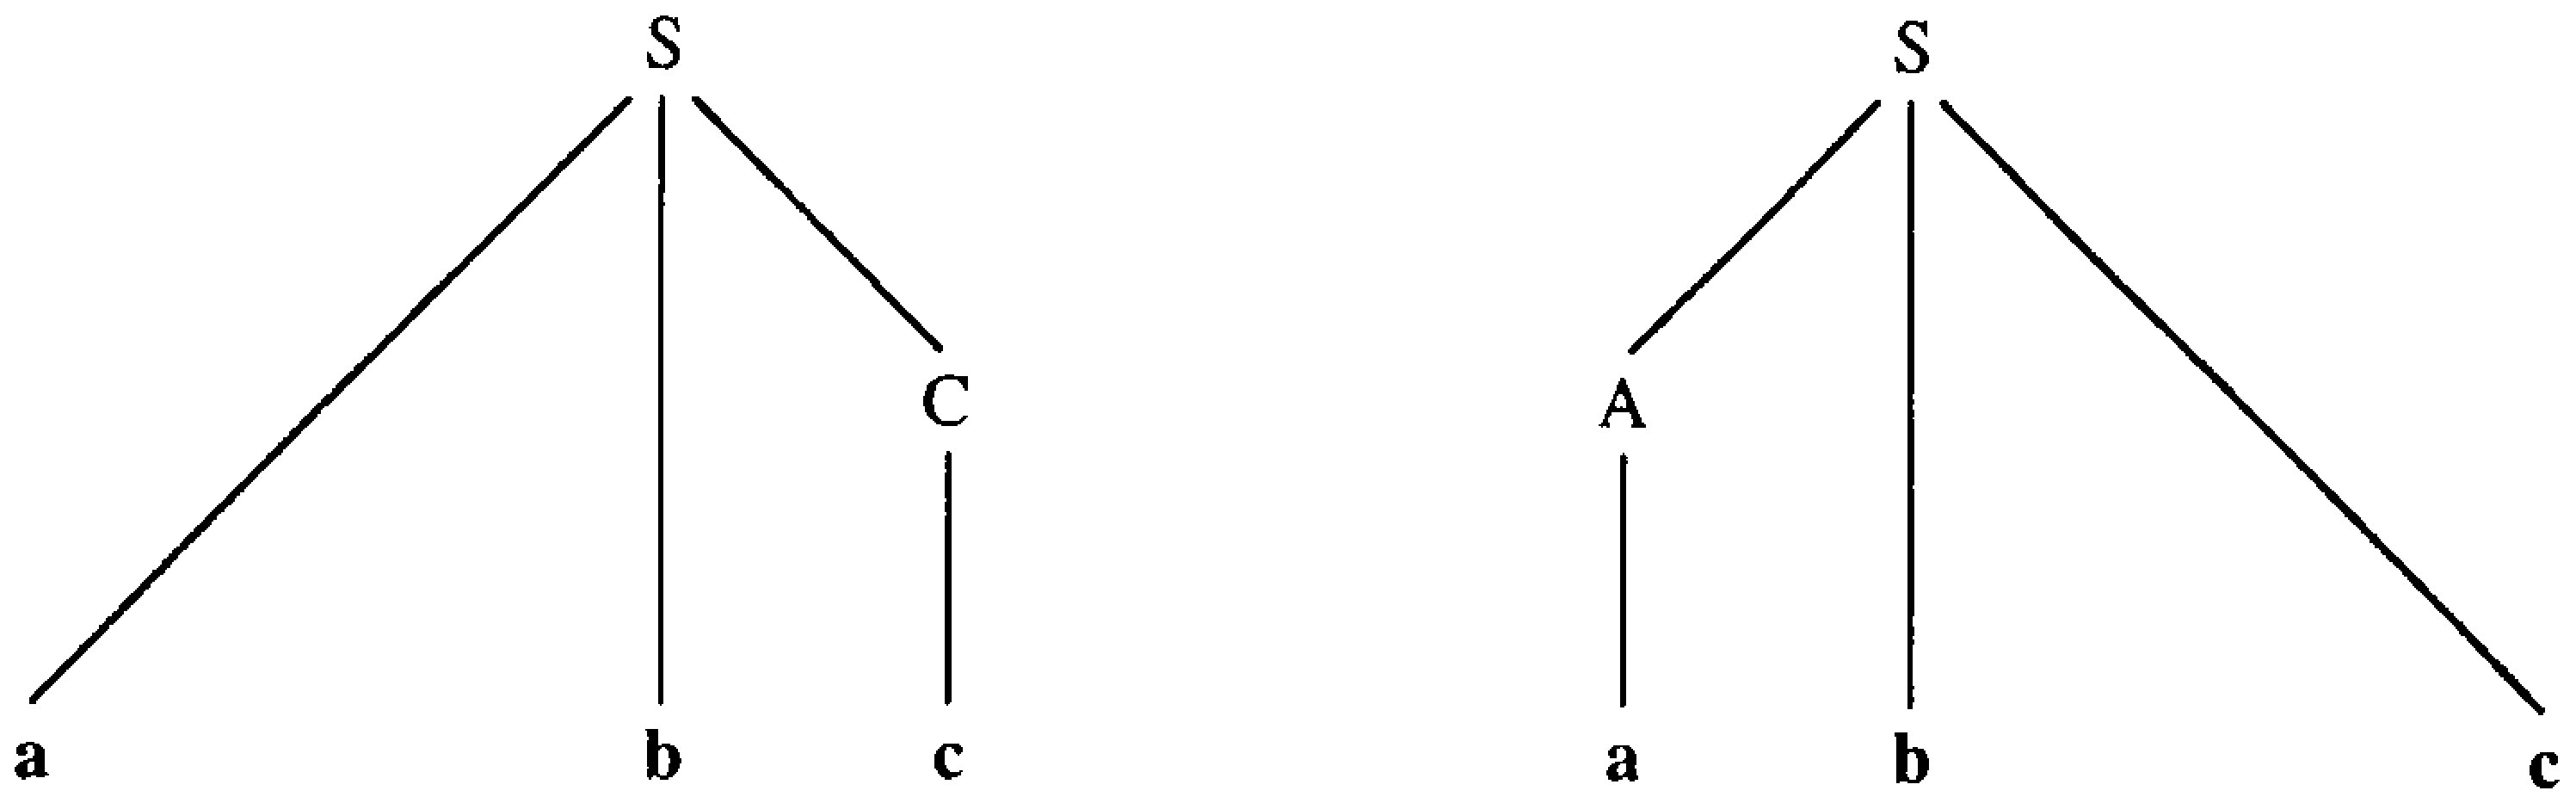
\epsfig{figure=ToFAfigures/fig9-8.eps,width=5.0in}}
\caption{The parse trees discussed in Example 9.8}\label{fig-9.8}
\end{figure}

% Corollary 9,1
\begin{cor}\label{cor-9.1}
The class \GSIG\ of languages generated by regular grammars is properly
contained in \USIG.

\emph{Proof.} Containment follows immediately from Theorem \ref{thm-9.2}. Proper
containment is demonstrated by the language and grammar discussed in Example 9.3.
\end{cor}

\subsection*{Example 9.9}

The right-linear grammar
\[ G_r = \langle\{S,B,C\},\{\pmb{a},\pmb{b},\pmb{c}\},S,\{S\rightarrow\pmb{a}B,
	S\rightarrow\pmb{ab}C,B\rightarrow\pmb{bc},C\rightarrow\pmb{c}\}\rangle \]
in Example 9.8 can be transformed, as outlined in Theorem \ref{thm-9.2}, into an
unambiguous grammar. The automaton corresponding to $G_r$ found by applying the
technique given in Lemma \ref{lmm-8.2} is shown in Figure \ref{fig-9.9}a. The version of this
automaton without lambda-moves (with the inaccessible states not shown) is
illustrated in Figure \ref{fig-9.9}b. The deterministic version, with the disconnected
states again removed, is given in Figure \ref{fig-9.9}c. For simplicity, the states are
relabeled in Figure \ref{fig-9.9}d. The corresponding grammar specified by Lemma \ref{lmm-8.1} is
\begin{center}\begin{tabular}{r@{ }l}
$G' =$ & $\langle\{S_0,S_1,S_2,S_3,S_4\},\{\pmb{a},\pmb{b},\pmb{c}\},S_0,\{S_0
	\rightarrow\pmb{a}S_1|\pmb{b}S_4|\pmb{c}S_4,S_1\rightarrow\pmb{a}S_4|
	\pmb{b}S_2|\pmb{c}S_4,$ \\
& $S_2\rightarrow\pmb{a}S_4|\pmb{b}S_4|\pmb{c}S_3,S_3\rightarrow\lambda|\pmb{a}
	S_4|\pmb{b}S_4|\pmb{c}S_4,S_4\rightarrow\pmb{a}S_4|\pmb{b}S_4|\pmb{c}S_4
	\}\rangle$
\end{tabular}\end{center}

% Figure 9.9
\begin{figure}
\centerline{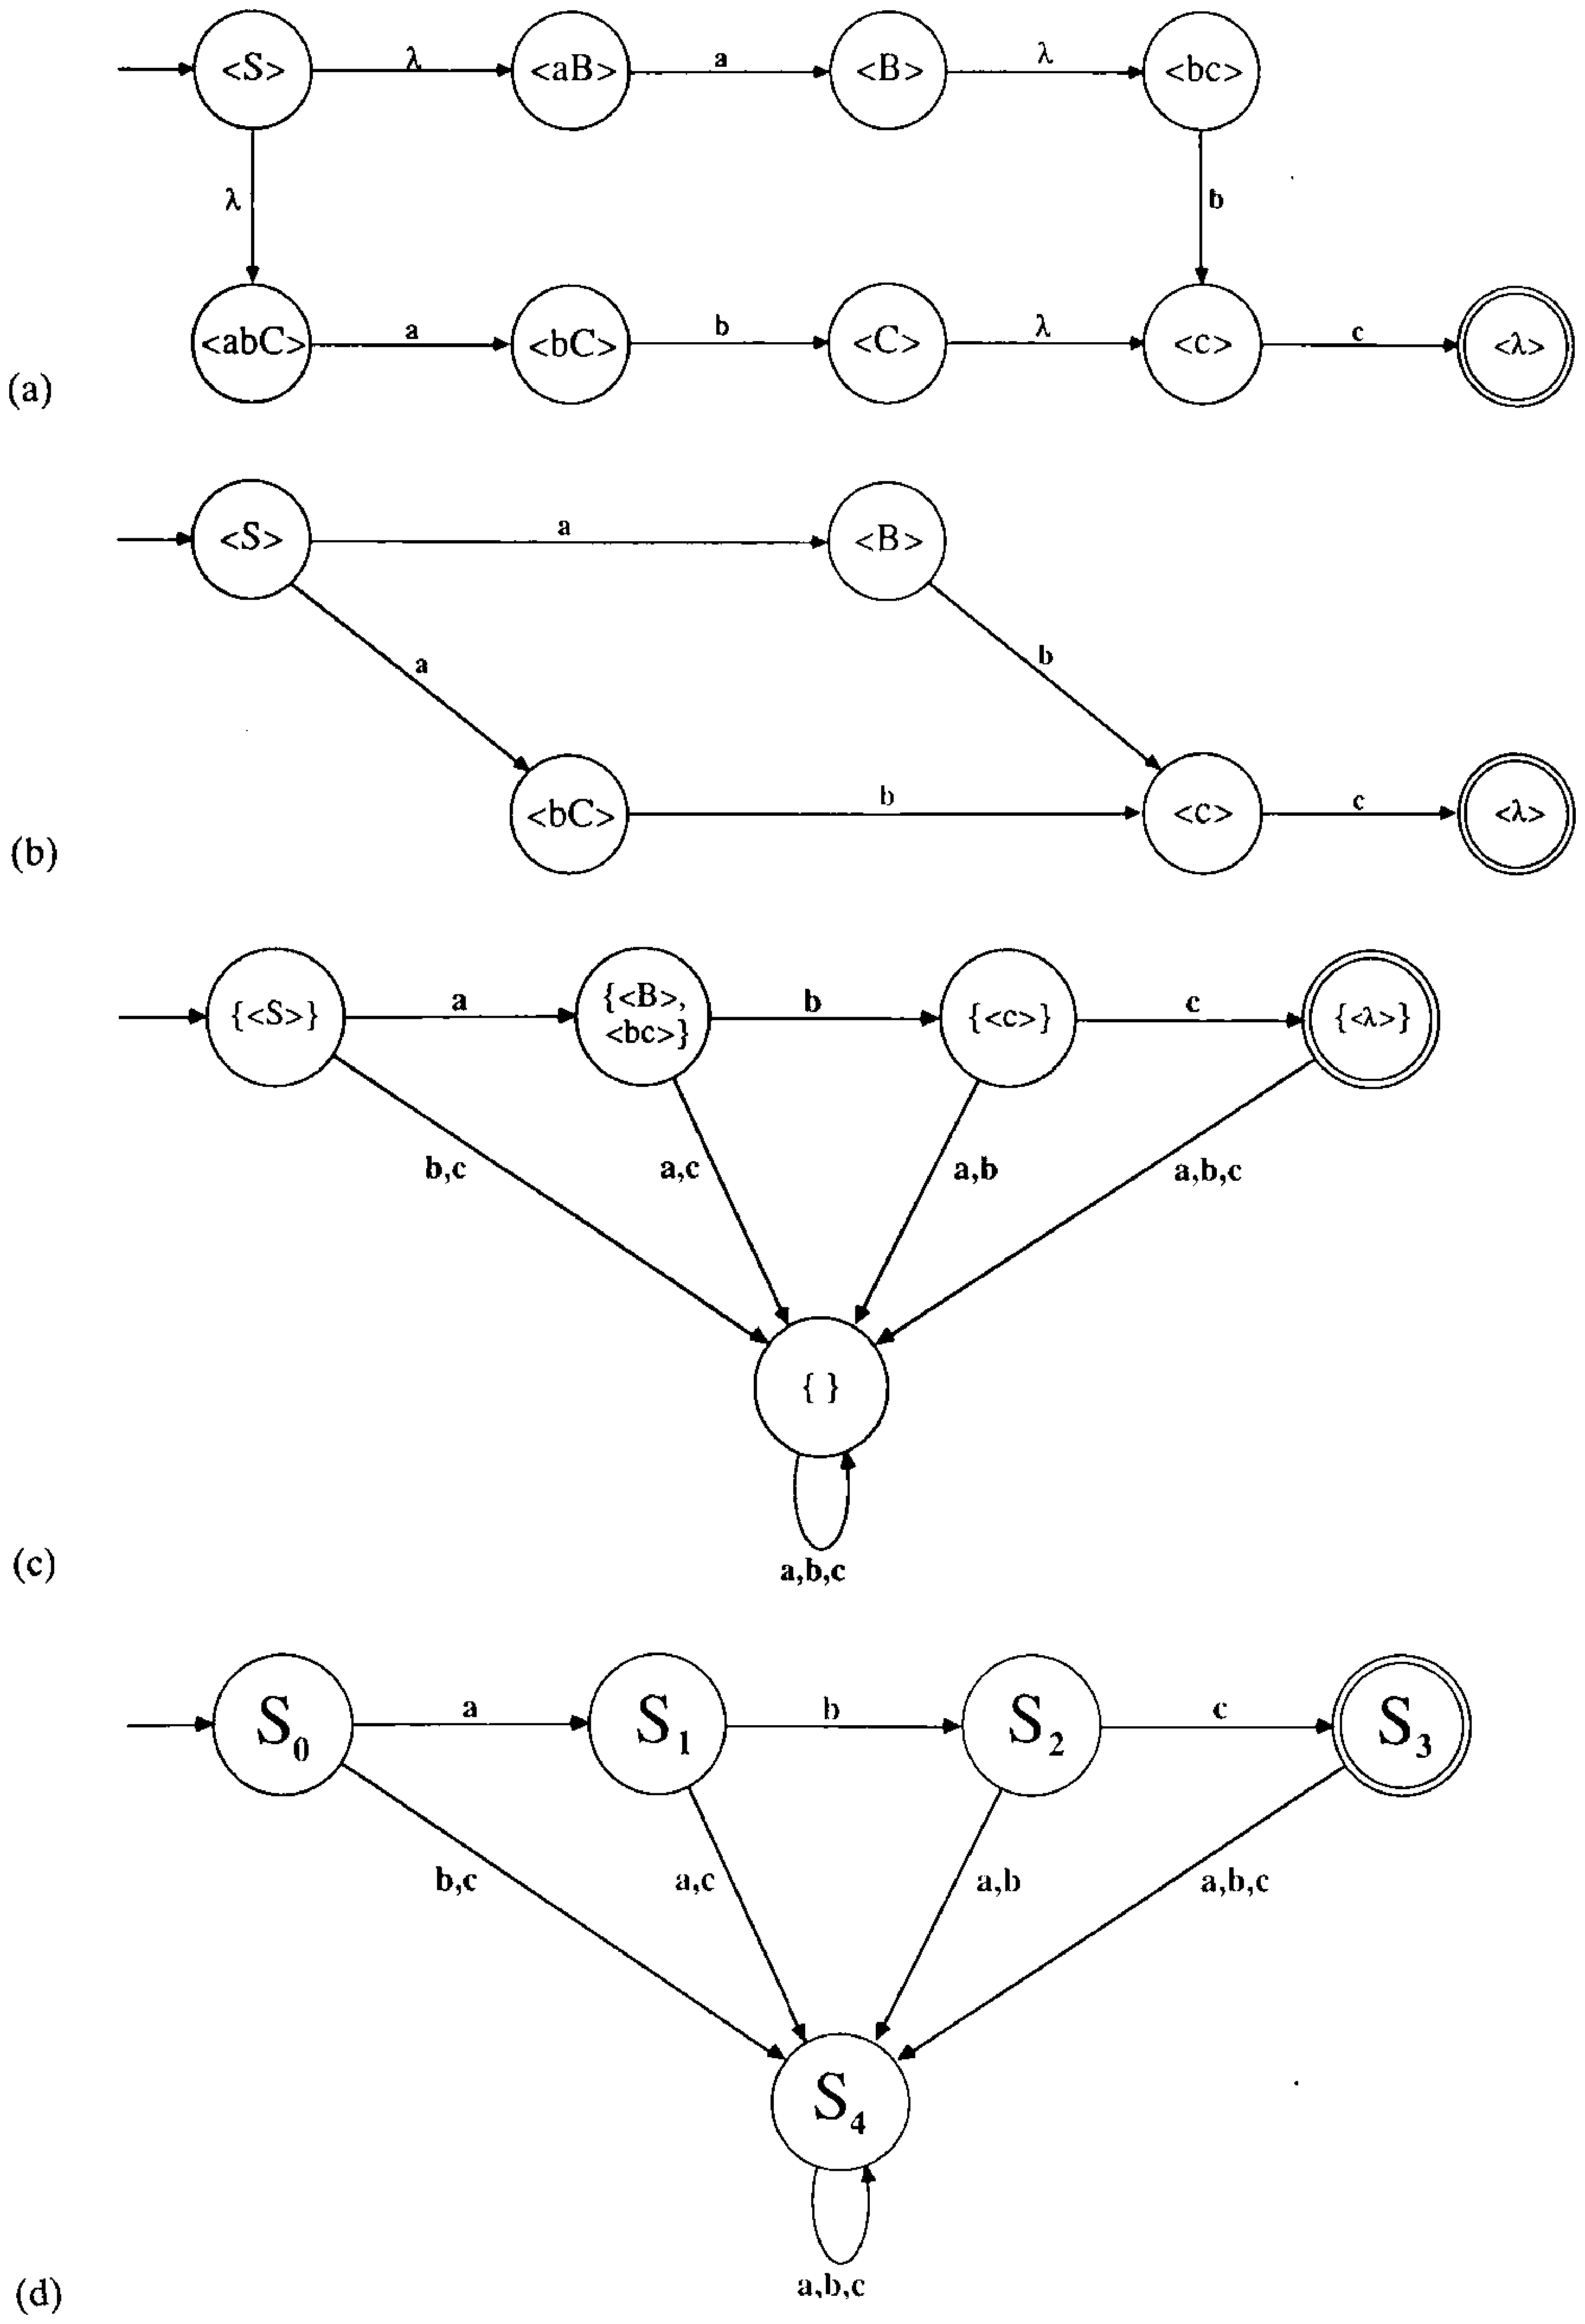
\epsfig{figure=ToFAfigures/fig9-9.eps,height=7.5in}}
\caption{(a) The automaton discussed in Example 9.9 (b) The simplified
automaton discussed in Example 9.9 (c) The deterministic automaton discussed
in Example 9.9 (d) The final automaton discussed in Example 9.9}\label{fig-9.9}
\end{figure}

The orderly nature of this resulting type of grammar easily admits the
specification of an algorithm that scans a proposed terminal string and builds
the corresponding parse tree. The partial parse tree for a string such as {\bf
abb} would be as pictured in Figure \ref{fig-9.10}a. This would clearly be an invalid
string since $S_4$ cannot be replaced by $\lambda$. By contrast, the tree for
the word $\pmb{abc}$ would produce a complete parse tree, and it is instructive to
step through the process by which it is built. The root of the tree must be
labeled $S_0$, and scanning the first letter of the word $\pmb{abc}$ is sufficient
to determine that the first production to be applied is $S_0\rightarrow\pmb{a}S_1$
(since no other $S_0$-rule immediately produces an $\pmb{a}$). Scanning the next
letter provides enough information to determine that the next $S_1$ rule that is
used must be $S_1\rightarrow\pmb{b}S_2$, and the third letter admits the
production $S_2\rightarrow\pmb{c}S_3$ and no other. Recognizing the end of the
string causes a check for whether the current non terminal can produce the empty
string. Since $S_3\rightarrow\lambda$ is in the grammar, the string $\pmb{abc}$ is
a valid terminal string, and corresponds to the parse tree shown in Figure \ref{fig-9.10}b.

% Figure 9.10
\begin{figure}
\centerline{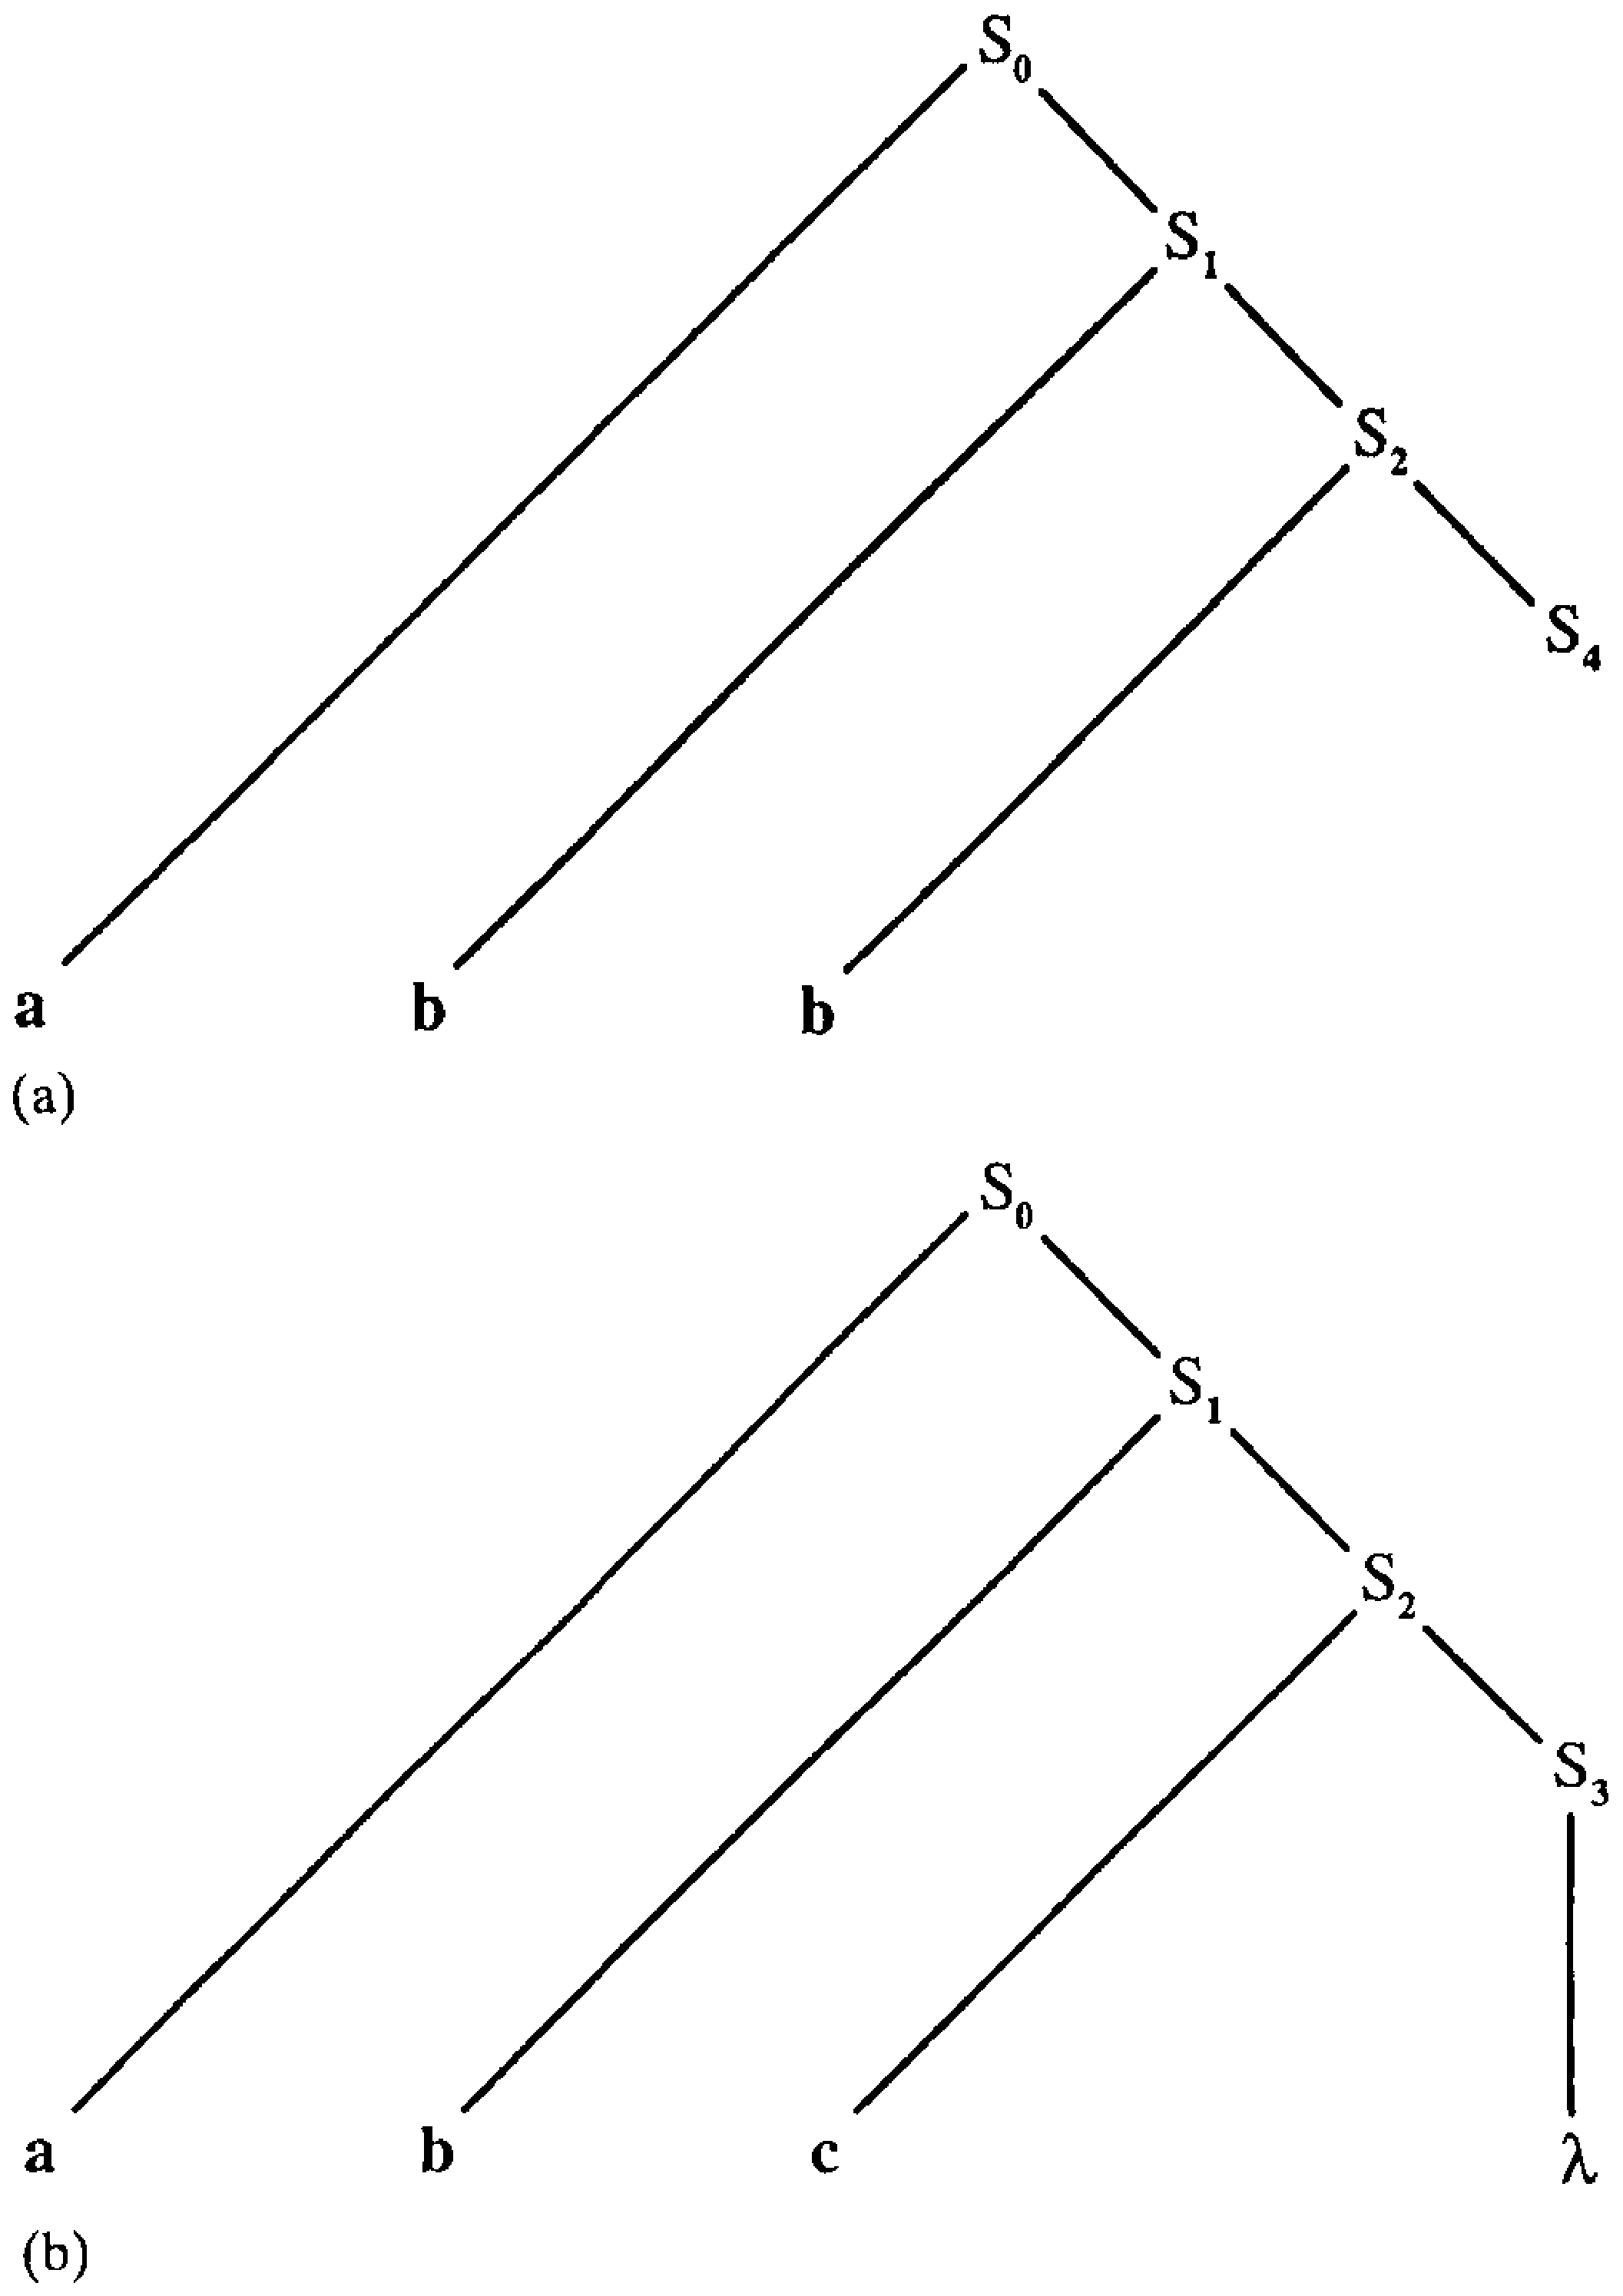
\epsfig{figure=ToFAfigures/fig9-10.eps,height=3.7in}}
\caption{(a) The partial parse tree for the string $\pmb{abb}$ (b) The parse tree
for the string $\pmb{abc}$}\label{fig-9.10}
\end{figure}

Grammars that admit scanning algorithms like the one outlined above are called
\Index{LL0} grammars since the parse tree can be deduced using a \underline{l}eft-to-right
scan of the proposed string while looking ahead \underline{0} symbols to produce
a \underline{l}eftmost derivation. That is, the production that produces a given
symbol can be immediately determined without regard to the symbols that follow.

Note that the grammar $G_3=\langle\{T\},\{\pmb{a}\},T,\{T\rightarrow\pmb{aaa}T,
T\rightarrow\pmb{aa}\}\rangle$ is LL2; that is, upon seeing $\pmb{a}$, the scanner
must look ahead two symbols to see if the end-of-string marker is imminent. In
this grammar, $\pmb{a}$ may be produced by either of the two $T$-rules; the
letters following this symbol in the proposed string are an important factor in
determining which production must be applied. The language described by $G_3$ is
simple enough to be defined by a grammar that is LL0, since every regular
grammar can be transformed as suggested by the proof of Theorem \ref{thm-9.2}.

The deterministic orderliness of LL0 grammars may be generally unattainable,
but it represents a desirable goal that a compiler designer would strive to
approximate when specifying a grammatical model of a programming language.
When a grammar is being defined to serve as a guide to construct a compiler,
an LL0 grammar is clearly the grammar of choice. Indeed, if even a portion of a
context-free grammar conforms to the LL0 property, this is of considerable
benefit. Whereas the technique outlined in Theorem \ref{thm-9.2} could be applied to any
regular language to find a hospitable LL0 grammar, programming languages are
generally more complex than regular languages, and these languages are unlikely
to have LL0 models. For context-free languages, it is much more likely that it
will not be possible to immediately determine which production (or sequence of productions)
will produce the symbol currently being scanned. In such cases, it will be
necessary to look ahead to successive symbols to make this determination.

A classic example of the need to look ahead in parsing programming languages
is reflected in the following FORTRAN statement:
\[ \mathtt{DO\ 77\ I=\ 1.5} \]\index{DO loop lookahead}
Since FORTRAN allows blanks within identifiers, this is a valid statement and
should cause the variable D077I to be assigned the value 1.5. On the other
hand, the statement
\[ \mathtt{DO\ 77\ I=\ 1,5} \]
specifies a ``do'' loop, and has an entirely different meaning. A lexical
analyzer that sees the three characters `$\mathtt{DO\ \ }$' cannot immediately determine
whether this represents a token for a do loop, or is instead part of a variable
identifier. It may have to wait until well after the equal sign is scanned to
correctly identify the tokens.

\section{Canonical Forms}\label{sec-9.3}

The definition of a context-free grammar was quite broad, and it is desirable
to establish canonical forms that will restrict the type of productions that can
be employed. Unrestricted context-free grammars do not admit very precise
relationships between the strings generated by the grammar and the production
sequences generating those strings. In particular, the length of a terminal
string may bear very little relation to the number of productions needed to
generate that string.

\subsection*{Example 9.10}

A string of length 18 can be generated with only three applications of
productions from the grammar
\[ \langle\{S\},\{\pmb{a},\pmb{b},\pmb{c}\},S,\{S\rightarrow\pmb{abcabc}S,S
	\rightarrow\pmb{abcabc}\}\rangle \]
A string of length 1 can be generated by no less than five productions in the
grammar
\[ \langle\{S_1,S_2,S_3,S_4,S_5\},\{\pmb{a},\pmb{b},\pmb{c}\},S_1,\{S_1\rightarrow
	S_2,S_2\rightarrow S_3,S_3\rightarrow S_4,S_4\rightarrow S_5,S_5
	\rightarrow\pmb{a}\} \]
It should be clear that even more extreme examples can be defined, in which the
number of terminal symbols markedly dominates the number of productions, and
vice versa.

The pumping theorem for context-free grammars (Theorem \ref{thm-9.7}) and other theorems
hinge on a more precise relationship between the number of terminal symbols
produced and the number of productions used to produce those symbols. Grammars
whose production sets satisfy more rigorous constraints are needed if such
relationships are to be guaranteed. The constraints should not be so severe that
some context-free languages cannot be generated by a set of productions that
conform to the restrictions. In other words, some well-behaved \emph{normal}
forms are sought.

A practical step toward that goal is the abolition of productions that cannot
participate in valid derivations. The algorithm for identifying such productions
constitutes an application of the algorithms developed previously for finite
automata. The following definition formally identifies productions that cannot
participate in valid derivations.

% Definition 9.7
\begin{dfn}\label{dfn-9.7}
A production $A\rightarrow\beta$ in a context-free grammar $G=\langle\Omega,
\Sigma,S,P\rangle$ is \emph{\Index{useful}} if it is part of a derivation
beginning with the start symbol and ending with a terminal string. That is, the
$A$-rule $A\rightarrow\beta$ is useful if there is a derivation $S\ \DRightarrow
\alpha A\omega\Rightarrow\alpha\beta\omega\ \DRightarrow x$, where $x\in\Sigma^*$.

\begin{quote}
A production that is not useful is called \emph{\Index{useless}}. \\
A nonterminal that does not appear in any useful production is called
	\emph{useless}. \\
A nonterminal that is not useless is called \emph{\Index{useful}}.
\end{quote}
\end{dfn}

\subsection*{Example 9.11}

Consider the grammar with productions
\begin{center}\begin{tabular}{r@{ $\rightarrow$ }l}
$S$ & $\pmb{g}A\pmb{e}, S\rightarrow\pmb{a}YB, S\rightarrow CY$ \\
$A$ & $\pmb{b}BY, A\rightarrow\pmb{oo}C$ \\
$B$ & $\pmb{dd}, B\rightarrow D$ \\
$C$ & $\pmb{j}VB, C\rightarrow\pmb{gi}$ \\
$D$ & $\pmb{n}$ \\
$U$ & $\pmb{k}W$ \\
$V$ & $\pmb{ba}XXX, V\rightarrow\pmb{o}V$ \\
$W$ & $\pmb{c}$ \\
$X$ & $\pmb{f}V$ \\
$Y$ & $Y\pmb{hm}$
\end{tabular}\end{center}
This grammar illustrates the three basic ways a nonterminal can qualify as
useless.
\begin{enumerate}
\item For the nonterminal $W$ above, it is impossible to find a derivation from
the start symbol $S$ that produces a sentential form containing $W$. $U$ also
lacks this quality.
\item No derivation containing the nonterminal $Y$ can produce a \emph{terminal}
string. $X$ and $V$ are likewise useless for the same reason.
\item $B$ is only produced in conjunction with useless nonterminals, and it is
therefore useless also. Once $B$ is judged useless, $D$ is seen to be useless
for similar reasons.
\end{enumerate}

% Theorem 9.3
\begin{thm}\label{thm-9.3}
Every nonempty context-free language $L$ can be generated by a context-free
grammar that contains no useless productions and no useless nonterminals.

\emph{Proof.} Note that if $L$ were empty the conclusion would be impossible to
attain: the start symbol would be useless, and every grammar by definition must
have a start symbol. Assume that $L$ is a nonempty context-free language. By
Definition \ref{dfn-8.6}, there is a context-free grammar $G=\langle\Omega,\Sigma,S,P
\rangle$ that generates $L$. The desired grammar $G^u$ can be formed from $G$,
with the useless productions removed from $P$ and the useless nonterminals
removed from $\Omega$. The new grammar $G^u$ will be equivalent to $G$, since
the lost items were by definition unable to participate in significant
derivations. $G^u$ will then obviously contain no useless productions and no
useless nonterminals.

A grammar with the desired properties must therefore exist, but the outlined
argument does not indicate \emph{how} to identify the items that must be removed.
The following algorithm, based on the procedures used to investigate finite
automata, shows how to effectively transform a context-free grammar $G$ into an
equivalent context-free grammar $G^u$ with no useless items.

Several nondeterministic finite automata over the (unrelated) alphabet $\{\pmb{1}\}$
will be considered, each identical except for the placement of the start state.
The states of the NDFA correspond to nonterminals of the grammar, and one extra
state, denoted by $\omega$, is added to serve as the only final state. A
transition from $A$ to $C$ will arise if a production in $P$ allows $A$ to be
replaced by a string containing the nonterminal $C$. States corresponding to
nonterminals that directly produce terminal strings will also have transitions
to the sole final state $\omega$. Formally, for the grammar $G=\langle\Omega,
\Sigma,S,P\rangle$ and any nonterminal $B\in\Omega$, define the NDFA $A^B =
\langle\{\pmb{1}\},\Omega\cup\{\omega\},B,\delta,\{\omega\}\rangle$, where
$\delta$ is defined by $\delta(\omega,\pmb{1})=\emptyset$, and for each $A \in
\Omega$, let
\[ \delta(A,\pmb{1})=\{C|(C\in\Omega\wedge(\exists\alpha,\gamma\in(\Omega\cup
	\Sigma)^*)(A\rightarrow\alpha C\gamma\in P))\}\cup\{\omega\} \]
if $(\exists\alpha\in\Sigma^*)(A\rightarrow\alpha\in P)$, and
\[ \delta(A,\pmb{1})=\{C|(C\in\Omega\wedge(\exists\alpha,\gamma\in(\Omega\cup
	\Sigma)^*)(A\rightarrow\alpha C\gamma\in P))\} \]
otherwise.

Note that, for any two nonterminals $R$ and $Q$ in $\Omega,\ A^R$ and $A^Q$ are
identical except for the specification of the start state. The previously
presented algorithms for determining the set of connected states in an automaton
can be applied to these new automata to identify the useless nonterminals. As
noted before, there are three basic ways a nonterminal can qualify as useless.
The inaccessible states in the NDFA $A^S$ correspond to nonterminals of the
first type and can be eliminated from both the grammar and the automata. For
each remaining nonterminal $B$, if the final state $\omega$ is not accessible
in $A^B$, then $B$ is a useless nonterminal of the second type and can be
eliminated from further consideration in both the grammar and the automata.
Checking for disconnected states in the pared-down version of $A^S$ will
identify useless nonterminals of the third type. The process can be repeated
until no further disconnected states are found.
\end{thm}

\subsection*{Example 9.12}

Consider again the grammar introduced in Example 9.11. The structure of each
of the automata is similar to that of $A^S$, shown in Figure \ref{fig-9.11}a. Note that
the disconnected states are indeed $W$ and $U$, which can be eliminated from the
state transition table. Checking the accessibility of $\omega$ in $A^S$, $A^A$,
$A^B$, $A^C$, and $A^D$ result in no changes, but $V$, $X$, and $Y$ are
eliminated when $A^V$, $A^X$, and $A^Y$ are examined, resulting in the automaton
displayed in Figure \ref{fig-9.11}b. Eliminating transitions associated with the
corresponding useless productions yields the automaton shown in Figure \ref{fig-9.11}c.
Checking for disconnected states in this machine reveals the remaining
inaccessible states. Thus, the equivalent grammar $G^u$ with no useless
nonterminals contains only the productions $S\rightarrow\pmb{g}A\pmb{e}$, $A
\rightarrow\pmb{ooC}$, and $C\rightarrow\pmb{gi}$.

Note that the actual language described by the NDFA $A^S$ is of no consequence,
nor may any finite automaton be capable of producing the context-free language
in question. However, the above method illustrates that the tools developed for
automata can be brought to bear in areas that do not directly apply to FAD
languages. A more efficient algorithm for identifying useless nonterminals can
be found in [HOPC]. If computerized, such a tailored algorithm would consume
less CPU time than if the automata modules described above were employed. In
terms of the programming effort required, though, it is often more advantageous
to adhere to the ``toolbox approach'' and adapt existing tools to new situations.

% Figure 9.11
\begin{figure}
% perhaps scale this one by height?  Get too big, it overwrites the page number.
\centerline{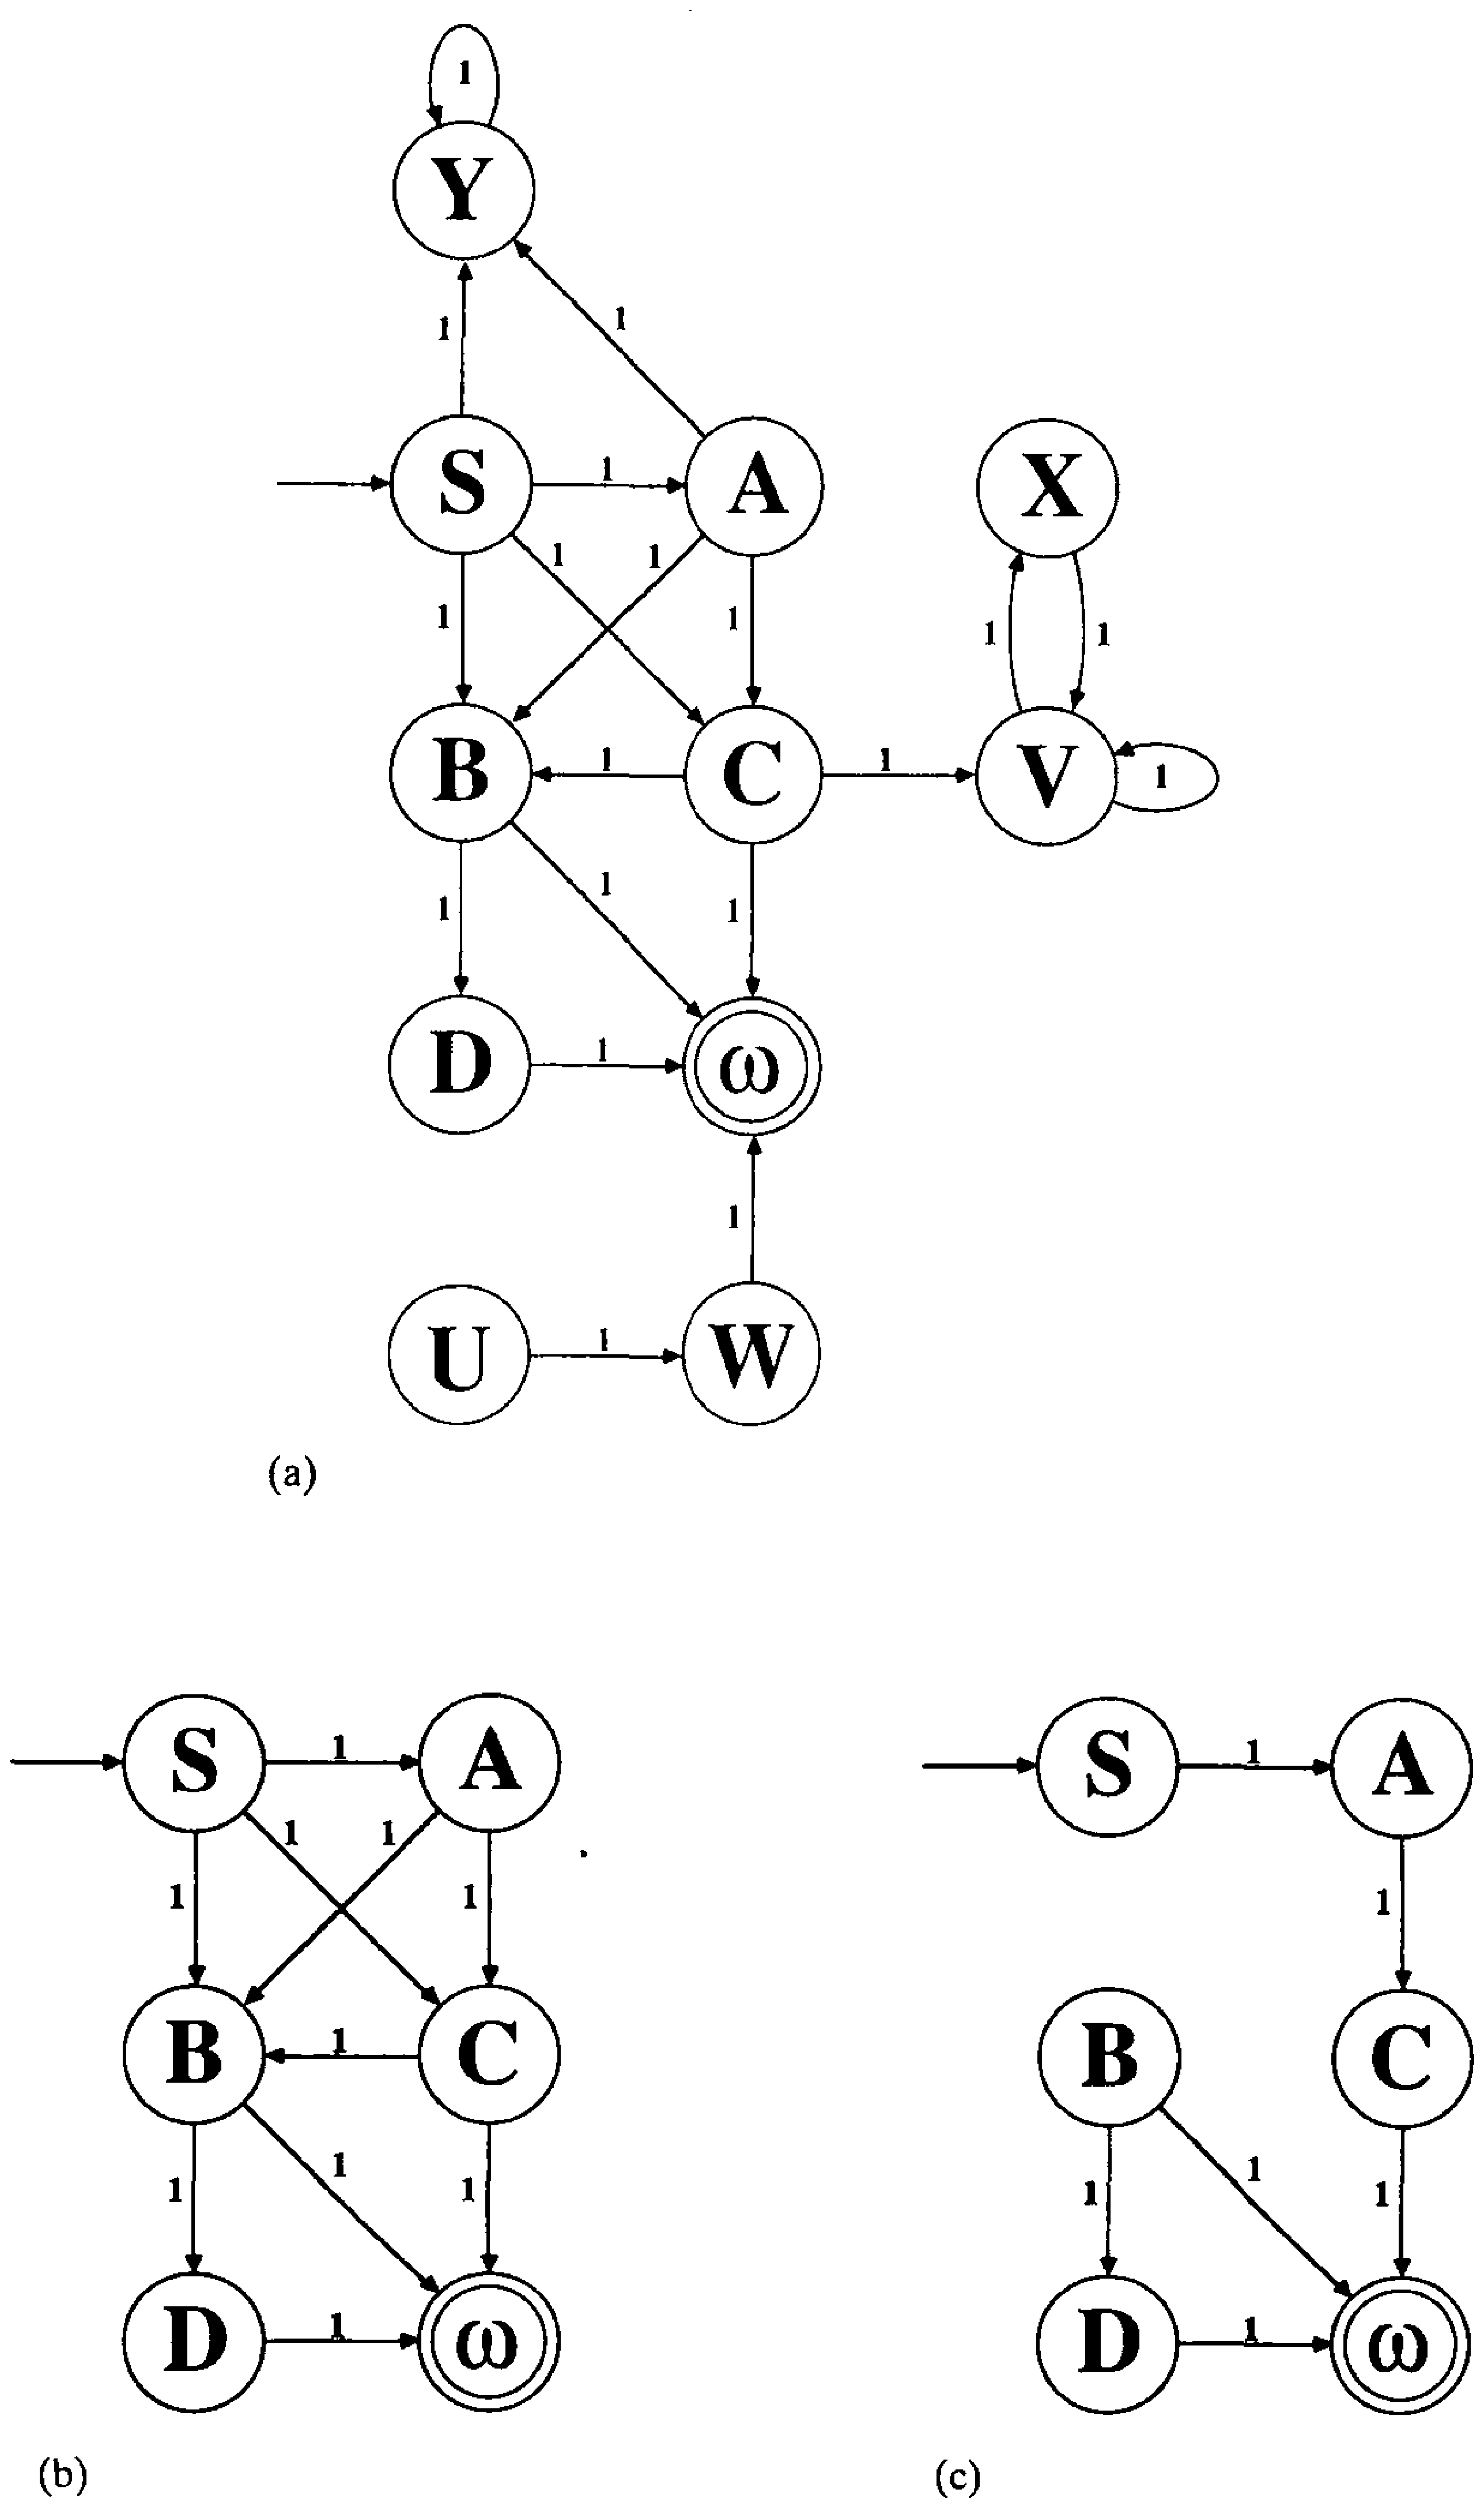
\epsfig{figure=ToFAfigures/fig9-11.eps,width=4.7in}}
\caption{(a) The automaton discussed in Example 9.12 (b) The simplified
automaton discussed in Example 9.12 (c) The final automaton discussed in
Example 9.12}\label{fig-9.11}
\end{figure}

Note that the algorithm developed in Theorem \ref{thm-9.3} relied on connectedness, and
hence the specification of the final states was unimportant in this approach.
With $\omega$ as the lone final state, some of the decision algorithms developed
in Chapter \ref{ch-12} could have been used in place of the connectivity and
accessibility checks.

Example 9.12 illustrates the simplification that can be attained by the
elimination of useless productions. Further convenience is afforded by the
elimination of nongenerative $A$-rules of the form $A\rightarrow B$. Recall that
in the grammar $\langle\{S_1,S_2,S_3,S_4,S_5\},\{\pmb{a},\pmb{b},\pmb{c}\},S_1,
\{S_1\rightarrow S_2,S_2\rightarrow S_3,S_3\rightarrow S_4,S_4\rightarrow S_5,
S_5\rightarrow\pmb{a}\}\rangle$, all the nonterminals were useful, but the
production set was still needlessly complex.

% Definition 9.8
\begin{dfn}\label{dfn-9.8}
A production of the form $A\rightarrow B$, where $A,B\in\Omega$, is called a
\emph{\Index{unit production}} or a \emph{\Index{nongenerative production}}.
\end{dfn}

As with the elimination of useless nonterminals, unit productions can be removed
with the help of automata constructs. The interested reader is referred to
[DENN] for the constructive proof. The proof given below indicates the general
algorithmic approach.

% Theorem 9.4
\begin{thm}\label{thm-9.4}
Every pure context-free language $L$ can be generated by a pure context-free
grammar which contains no useless non-terminals and no unit productions. Every
context-free language $L'$ can be generated by a context-free grammar which
contains no useless non-terminals and no unit productions except perhaps the
$Z$-rule $Z\rightarrow S$, where $Z$ is the new start symbol.

\emph{Proof.} If the first statement of the theorem is proved, the second will
follow immediately from Definition \ref{dfn-8.6}. If $L$ is a pure context-free language,
then by Definition \ref{dfn-8.5} there is a pure context-free grammar $G=\langle\Omega,
\Sigma,S,P\rangle$ that generates $L$. Divide the production set up into $P^u$
and $P^n$, the set of unit productions and the set of nonunit productions,
respectively. For each nonterminal $B$ found in $P^u$, find $B^u=\{C|B
\DRightarrow C\}$, the \emph{unit closure} of $B$. The derivations sought must
all come from the (finite) set $P^u$, and there is clearly an algorithm that
correctly calculates $B^u$. In fact, $B^u$ is represented by the set of
accessible states in a suitably defined automaton (see the exercises). Define a
new grammar $G'=\langle\Omega,\Sigma,S,P'\rangle$, where $P'=P^n\cup\{B
\rightarrow\alpha|B$ is a nonterminal in $P^u\wedge C\in B^u\wedge C\rightarrow
\alpha\in P^n\}$. A straightforward induction argument shows that $G'$ is
equivalent to $G$, and $G'$ contains no unit productions. Note that if $G$ is
pure, so is $G'$.

G' is likely to contain useless nonterminals, even if all the productions in $G$
were useful (see Example 9.13). However, the algorithm from Theorem \ref{thm-9.3} can now
be applied to $G'$ to eliminate useless nonterminals. Since that algorithm
creates no new productions, the resulting grammar will still be free of unit
productions.
\end{thm}

\subsection*{Example 9.13}

Consider again the pure context-free grammar
\[ \langle\{S_1,S_2,S_3,S_4,S_5\},\{\pmb{a},\pmb{b},\pmb{c}\},S_1,\{S_1
	\rightarrow S_2,S_2\rightarrow S_3,S_3\rightarrow S_4,S_4\rightarrow
	S_5,S_5\rightarrow\pmb{a}\}\rangle \]
The production set is split into $P^n = \{S_5\rightarrow\pmb{a}\}$ and
\[ P^u = \{S_1\rightarrow S_2,S_2\rightarrow S_3,S_3\rightarrow S_4,S_4
	\rightarrow S_5\}. \]
The unit-closure sets are
\begin{center}\begin{tabular}{r@{ = }l}
$S^u_1$ & $\{S_1,S_2,S_3,S_4,S_5\}$ \\
$S^u_2$ & $\{S_2,S_3,S_4,S_5\}$ \\
$S^u_3$ & $\{S_3,S_4,S_5\}$ \\
$S^u_4$ & $\{S_4,S_5\}$ \\
$S^u_5$ & $\{S_5\}$
\end{tabular}\end{center}
Since $S_5\rightarrow\pmb{a}$ and $S_5\in S^u_3$, the production $S_3\rightarrow
\pmb{a}$ is added to $P'$. The full set of productions is $P'=\{S_1\rightarrow
\pmb{a},S_2\rightarrow\pmb{a},S_3\rightarrow\pmb{a},S_4\rightarrow\pmb{a},S_5
\rightarrow\pmb{a}\}$. The elimination of useless nonterminals and productions
results in the grammar $\langle\{S_1\},\{\pmb{a},\pmb{b},\pmb{c}\},S_1,\{S_1
\rightarrow\pmb{a}\}\rangle$.

\subsection*{Example 9.14}

Consider the context-free grammar with productions
\begin{center}\begin{tabular}{r@{ $\rightarrow$ }l}
$Z$ & $S,\ Z\rightarrow\lambda$ \\
$S$ & $CB\pmb{h},\ S\rightarrow D$ \\
$A$ & $\pmb{aa}C$ \\
$B$ & $S\pmb{f},\ B\rightarrow\pmb{ggg}$ \\
$C$ & $\pmb{c}A,\ C\rightarrow\pmb{d},C\rightarrow C$ \\
$D$ & $E,\ D\rightarrow SABC$ \\
$E$ & $\pmb{be}$
\end{tabular}\end{center}
The unit closures of each of the appropriate nonterminals and the new
productions they imply are shown below. Note that $Z\rightarrow S$ is not
considered and that the productions suggested by $C\rightarrow C$ are already
present.
\begin{center}\begin{tabular}{r@{ \ $\DRightarrow$ }l@{$\qquad$}r@{ $\rightarrow$ }l}
$S$ & $D$ & $S$ & $SABC$ \\
$S$ & $E$ & $S$ & $\pmb{be}$ \\
$D$ & $E$ & $D$ & $\pmb{be}$ \\
$C$ & $C$ & $C$ & $\pmb{c}A,\ C\rightarrow\pmb{d}$
\end{tabular}\end{center}
The new set of productions is therefore
\begin{center}\begin{tabular}{r@{ $\rightarrow$ }l}
$Z$ & $S,\ Z\rightarrow\lambda$ \\
$S$ & $SABC,\ S\rightarrow\pmb{be},\ S\rightarrow CB\pmb{h}$ \\
$A$ & $\pmb{aa}C$ \\
$B$ & $S\pmb{f},\ B\rightarrow\pmb{ggg}$ \\
$C$ & $\pmb{c}A,\ C\rightarrow\pmb{d}$ \\
$D$ & $\pmb{be},\ D\rightarrow SABC$ \\
\end{tabular}\end{center}
Note that D is now useless and can be eliminated.

The assurance that every context-free grammar corresponds to an equivalent
grammar with no unit productions is helpful in many situations. In particular,
it is instrumental to the proof showing that the following restrictive type of
grammar is indeed a canonical form for context-free languages.

% Definition 9.9
\begin{dfn}\label{dfn-9.9}
A pure context-free grammar $G=\langle\Omega,\Sigma,S,P\rangle$ is in
\emph{pure Chomsky normal form}\index{pure Chomsky normal form|see{PCNF}} (\Index{PCNF}) if $P$ contains only
productions of the form $A\rightarrow BC$ and $A\rightarrow\pmb{d}$, where $B$
and $C$ are nonterminals and $\pmb{d}\in\Sigma$.

A context-free grammar $G=\langle\Omega,\Sigma,Z,P\rangle$ is in
\emph{Chomsky normal form}\index{Chomsky normal form|see{CNF}}(\Index{CNF}) if the $Z$-rules $Z\rightarrow
S$ and $Z\rightarrow\lambda$ are the only allowable productions involving the
start symbol $Z$, and all other productions are of the form $A\rightarrow BC$
and $A\rightarrow\pmb{d}$, where $B$ and $C$ are nonterminals and $\pmb{d}\in
\Sigma$.
\end{dfn}

Thus, in PCNF the grammatical rules are limited to producing exactly two
nonterminals or one terminal symbol. Few of the grammars discussed so far have
met the restricted criteria required by Chomsky normal form. However, every
context-free grammar can be transformed into an equivalent CNF grammar, as
indicated in the following proof. The basic strategy will be to add new
nonterminals and replace undesired productions such as $A\rightarrow JK\pmb{cb}$
by a set of equivalent productions in the proper form, such as $A\rightarrow
JY_{11},\ Y_{11}\rightarrow KY_{12},\ Y_{12}\rightarrow X_cX_b,\ X_c\rightarrow
\pmb{c},\ X_b\rightarrow\pmb{b}$, where $Y_{11},\ Y_{12},\ X_b$, and $X_c$ are
new nonterminals.

% Theorem 9.5
\begin{thm}\label{thm-9.5}
\ \\
\indent Every pure context-free language $L$ can be generated by a pure Chomsky normal
form grammar.

Every context-free language $L'$ can be generated by a Chomsky
normal form grammar.

\emph{Proof.} Again, if the first statement of the theorem is proved, the second
will follow immediately from Definition \ref{dfn-8.6}. If L is a pure context-free
language, then by Definition \ref{dfn-8.5} there is a pure context-free grammar $G=\langle
\Omega,\Sigma,S,P\rangle$ that generates $L$. Theorem \ref{thm-9.4} shows that without
loss of generality we may assume that P contains no unit productions. We
construct a new grammar $G'=\langle\Omega,\Sigma,S,P'\rangle$ in the following
manner. Number the productions in $P$, and consider each production in turn. If
the right side of the $k$th production consists of only a single symbol, then it
must be a terminal symbol, since there are no unit productions. No modifications
are necessary in this case, and the production is retained for use in the new
set of productions $P'$. The same is true if the kth production consists of two
symbols and they are both nonterminals. If one or both of the symbols is a
terminal, then the rule must be modified by replacing any terminal symbol {\bf
a} with a new nonterminal $X_{\pmb{a}}$. Whenever such a replacement is done, a
production of the form $X_{\pmb{a}}\rightarrow\pmb{a}$ must also be included in
the new set of productions $P'$. If the $k$th production is $A\rightarrow\alpha_1
\alpha_2\alpha_3\cdots\alpha_n$, where the number of (terminal and nonterminal)
symbols is $n>2$, then new nonterminals $Y_{k1},Y_{k2},\ldots,Y_{kn-2}$ must be
introduced and the rule must be replaced by the set of productions $A\rightarrow
\alpha_1Y_{k1},Y_{k1}\rightarrow\alpha_2Y_{k2},Y_{k2}\rightarrow\alpha_3Y_{k3},
\cdots Y_{kn-2}\rightarrow \alpha_{n-1}\alpha_n$. Again, if any $\alpha_i$ is a
terminal symbol such as $\pmb{a}$, it must be replaced as indicated earlier by the
nonterminal $X_{\pmb{a}}$.

Each new set of rules is clearly capable of producing the same effect as the
rule that was replaced. Each nonterminal $Y_{ki}$ is used in only one such
replacement set to ensure that the new rules do not combine in unexpected new
ways. Tedious but straightforward inductive proofs will justify that $L(G) =
L(G')$.
\end{thm}

\subsection*{Example 9.15}

The grammar discussed in Example 9.14 can be transformed into CNF by the
algorithm given in Theorem \ref{thm-9.5}. After elimination of the unit productions and
the consequent useless productions, the productions (suitably numbered) that
must be examined are

\begin{tabular}{l@{$\qquad\qquad\qquad$}l}
$\pmb{1.}\ \ S\rightarrow SABC$ & $\pmb{5.}\ \ B\rightarrow S\pmb{f}$ \\
$\pmb{2.}\ \ S\rightarrow\pmb{be}$ & $\pmb{6.}\ \ B\rightarrow\pmb{ggg}$ \\
$\pmb{3.}\ \ S\rightarrow CB\pmb{h}$ & $\pmb{7.}\ \ C\rightarrow\pmb{c}A$ \\
$\pmb{4.}\ \ A\rightarrow\pmb{aa}C$ & $\pmb{8.}\ \ C\rightarrow\pmb{d}$
\end{tabular}

\noindent In the corresponding lists given below, notice that only production 8
is retained; the others are replaced by
\begin{center}\begin{tabular}{r@{ $\rightarrow$ }l}
$S$ & $SY_{11},\ Y_{11}\rightarrow AY_{12},\ Y_{12}\rightarrow BC$ \\
$S$ & $X_{\pmb{b}}X_{\pmb{e}}$ \\
$S$ & $CY_{31},\ Y_{31}\rightarrow BX_{\pmb{h}}$ \\
$A$ & $X_{\pmb{a}}Y_{41},\ Y_{41}\rightarrow X_{\pmb{a}}C$ \\
$B$ & $SX_{\pmb{f}}$ \\
$B$ & $X_{\pmb{g}}Y_{61},\ Y_{61}\rightarrow X_{\pmb{g}}X_{\pmb{g}}$ \\
$C$ & $X_{\pmb{c}}A$ \\
$C$ & $\pmb{d}$
\end{tabular}\end{center}
and the terminal productions $X_{\pmb{b}}\rightarrow\pmb{b},\ X_{\pmb{e}}
\rightarrow\pmb{e},\ X_{\pmb{h}}\rightarrow\pmb{h},\ X_{\pmb{a}}\rightarrow
\pmb{a},\ X_{\pmb{f}}\rightarrow\pmb{f},\ X_{\pmb{g}}\rightarrow\pmb{g}$. Since
$\pmb{d}$ did not appear as part of a two-symbol production, the rule $X_{\pmb{d}}
\rightarrow\pmb{d}$ can be eliminated. The above rules, with $S$ as the start
symbol, form a pure Chomsky normal form grammar. The new start symbol $Z$ and
productions $Z\rightarrow S$ and $Z\rightarrow\lambda$ would be added to this
pure context-free grammar to obtain the required CNF.

Grammars in Chomsky normal form allow an exact correspondence to be made between
the length of a terminal string and the length of the derivation sequence that
produces that string. If the empty string can be derived, the production
sequence will consist of exactly one rule application ($Z\rightarrow\lambda$). A
simple inductive argument shows that, if a string of length $n>0$ can be derived,
the derivation sequence must contain exactly $2n$ steps. In the grammar derived
in Example 9.15, for example, the following terminal string of length 5 is
generated in exactly ten productions:
\begin{center}\begin{tabular}{r@{ $\Rightarrow$ }l}
$Z$ & $S\Rightarrow CY_{31} \Rightarrow \pmb{d}Y_{31} \Rightarrow \pmb{d}BX_h
	\Rightarrow \pmb{d}SX_fX_h \Rightarrow \pmb{d}X_bX_eX_fX_h \Rightarrow
	\pmb{db}X_eX_fX_h$ \\
& $\pmb{dbe}X_fX_h \Rightarrow \pmb{dbef}X_h \Rightarrow \pmb{dbefh}$
\end{tabular}\end{center}

Other useful properties are also assured for grammars in Chomsky normal form.
When a grammar is in CNF, all parse trees can be represented by binary trees,
and upper and lower bounds on the depth of a parse tree for a string of length
$n$ can be found (see the exercises). The derivational relationship between the
number of production steps used and the number of terminals produced implies
that CNF grammars generate an average of one terminal every two productions. The
following canonical form requires every production to contain at least one
terminal symbol, and grammars in this form must produce strings of length
$n(>0)$ in no more than $n$ steps.

% Definition 9.10
\begin{dfn}\label{dfn-9.10}
A pure context-free grammar $G=\langle\Omega,\Sigma,S,P\rangle$ is in
\emph{\Index{pure Greibach normal form}} (\Index{PGNF}) if $P$ contains only 
productions of the form $A\rightarrow\pmb{d}\alpha$, where $\alpha\in(\Omega\cup
\Sigma)^*$ and $d\in\Sigma$..

A context-free grammar $G=\langle\Omega,\Sigma,Z,P\rangle$ is in \emph{\Index{Greibach
normal form}} (\Index{GNF}) if the $Z$-rules $Z\rightarrow S$ and $Z\rightarrow
\lambda$ are the only allowable productions involving the start symbol $Z$, and
all other productions are of the form $A\rightarrow\pmb{d}\alpha$, where $\alpha
\in(\Omega\cup\Sigma)^*$ and $\pmb{d}\in\Sigma$.
\end{dfn}

In pure Greibach normal form, the grammatical rules are limited to producing at
least one terminal symbol as the first symbol. The original grammar in Example
9.9 is a PGNF grammar, but few of the other grammars presented in this chapter
meet the seemingly mild restrictions required for Greibach normal form. The main
obstacle to obtaining a GNF grammar is the possible presence of \emph{left
recursion}. A nonterminal A is called \emph{\Index{left recursive}} if there is
a sequence of one or more productions for which $A\ \DRightarrow A\beta$ for some
string $\beta$. Greibach normal form disallows such occurrences since no
production may produce a string starting with a nonterminal. Replacing
productions involved with left recursion is complex, but every context-free
grammar can be transformed into an equivalent GNF grammar, as shown by Theorem
\ref{thm-9.6}. Two techniques will be needed to transform the productions into the
appropriate form, and the following lemmas ensure that the grammatical
transformations leave the language unchanged. The first indicates how to remove
an $X$-rule that begins with an undesired nonterminal; Lemma \ref{lmm-9.1} specifies a new
set of productions that compensate for the loss.

% Lemma 9.1
\begin{lmm}\label{lmm-9.1}
Let $G=\langle\Omega,\Sigma,S,P\rangle$ be a context-free grammar, and assume
there is a string $\alpha$ and nonterminals $X$ and $B$ for which $X\rightarrow
B\alpha\in P$. Further assume that the set of all $B$-rules is given by $\{B
\rightarrow\beta_1,B\rightarrow\beta_2,\ldots,B\rightarrow\beta_m\}$ and let
$G'=\langle\Omega,\Sigma,S,P'\rangle$, where
\[ P'=P\cup\{X\rightarrow\beta_1\alpha,X\rightarrow\beta_2\alpha,\ldots,X
	\rightarrow\beta_m\alpha\} - \{X\rightarrow B\alpha\}. \]
Then $L(G) = L(G')$.

\emph{Proof.} Let each nonterminal $A$ be associated with the set of sentential
forms $X_A$ that $A$ can produce. That is, let $A=X_A=\{x\in(\Sigma\cup\Omega)^*|
A\ \DRightarrow x\}$. The nonterminals then denote variables in a set of language
equations that reflect the productions in $P$. These equations will generally
not be linear; several variables may be concatenated together within a single
term. Since the set of all $B$-rules were $B\rightarrow\beta_1,B\rightarrow
\beta_2,\ldots,B\rightarrow\beta_m,X_B$ satisfies the equation
\[ X_B = \beta_1 \cup \beta_2 \cup \cdots \cup \beta_m \]
Similarly, if the $X$-rules other than $X\rightarrow B\alpha$ are $X\rightarrow
\gamma_1,X\rightarrow \gamma_2,\ldots,X\rightarrow\gamma_n$, then $X$ satisfies
the equation
\[ X_X = \gamma_1\cup\gamma_2\cup\cdots\cup\gamma_n\cup X_B\alpha \]
Substituting for $X_B$ in the $X_X$ equation yields
\[ X_X = \gamma_1\cup\gamma_2\cup\cdots\cup\gamma_n\cup(\beta_1\cup\beta_2\cup
	\cdots\cup\beta_m)\alpha \]
which by the distributive law becomes
\[ X_X = \gamma_1\cup\gamma_2\cup\cdots\cup\gamma_n\cup\beta_1\alpha\cup\beta_2
	\alpha\cup\cdots\cup\beta_m\alpha \]
This shows why the productions $X\rightarrow\beta_1\alpha,X\rightarrow\beta_2
\alpha, \ldots ,X\rightarrow\beta_m\alpha$ can replace the rule $X\rightarrow B
\alpha$.
\end{lmm}
The type of replacement justified by Lemma \ref{lmm-9.1} will not eliminate left recursion.
The following lemma indicates a way to remove all the left-recursive $X$-rules
by introducing a new right-recursive nonterminal.

% Lemma 9.2
\begin{lmm}\label{lmm-9.2}
Let $G=\langle\Omega,\Sigma,S,P\rangle$ be a context-free grammar, and choose a
nonterminal $X\in\Omega$. Denote the set of all left-recursive $X$-rules by $X^r =
\{X\rightarrow X\alpha_1,X\rightarrow X\alpha_2,\ldots,X\rightarrow X\alpha_m\}$
and the set of all non[left]recursive X-rules by $X^n=\{X\rightarrow\gamma_1,X
\rightarrow\gamma_2,\ldots,X\rightarrow\gamma_n\}$. Choose a new nonterminal $Y
\notin\Omega$ and let $G'' = \langle\Omega\cup\{Y\},\Sigma,S,P''\rangle$, where
$P'' = P\cup\{X\rightarrow\gamma_1Y,X\rightarrow\gamma_2Y,\ldots,X\rightarrow
\gamma_nY\}\cup\{Y\rightarrow\alpha_1,Y\rightarrow\alpha_2,\ldots,Y\rightarrow
\alpha_m\}\cup\{Y\rightarrow\alpha_1Y,Y\rightarrow\alpha_2Y,\ldots,Y\rightarrow
\alpha_mY\}-X^r$. Then $L(G) = L(G'')$.

\emph{Proof.} As in Lemma \ref{lmm-9.1}, let each nonterminal $A$ be associated with the
set of sentential forms $X_A$ that $A$ can produce, and consider the set of
language equations generated by $P$. The $X_X$ equation is
\[ X_X = \gamma_1 \cup \gamma_2 \cup\cdots\cup \gamma_n \cup X_X\alpha_1 \cup
	X_X\alpha_2 \cup\cdots\cup X_X\alpha_m \]
Solving by the method indicated in Theorem \ref{thm-6.4}c for an equivalent expression
for $X_X$ shows that
\[ X_X = (\gamma_1\cup\gamma_2\cup\cdots\cup\gamma_n)(\alpha_1\cup\alpha_2\cup
	\cdots\cup\alpha_m)^* \]
In the new set of productions $P''$, the equations of interest are
\begin{center}\begin{tabular}{l}
$X_X = \gamma_1\cup\gamma_2\cup\cdots\cup\gamma_n\cup\gamma_1X_Y\cup\gamma_2X_Y
	\cup\cdots\cup\gamma_nX_Y$ \\
$X_Y = \alpha_1\cup\alpha_2\cup\cdots\cup\alpha_m\cup\alpha_1X_Y\cup\alpha_2X_Y
	\cup\cdots\cup\alpha_mX_Y$
\end{tabular}\end{center}
Factoring each equation produces
\begin{center}\begin{tabular}{l}
$X_X = \gamma_1\cup\gamma_2\cup\cdots\cup\gamma_n\cup(\gamma_1\cup\gamma_2\cup
	\cdots\cup\gamma_n)X_Y$ \\
$X_Y = \alpha_1\cup\alpha_2\cup\cdots\cup\alpha_m\cup(\alpha_1\cup\alpha_2\cup
	\cdots\cup\alpha_m)X_Y$
\end{tabular}\end{center}
and the second can also be solved for an equivalent expression for $X_Y$,
yielding
\[ X_Y = (\alpha_1\cup\alpha_2\cup\cdots\cup\alpha_m)^*(\alpha_1\cup\alpha_2\cup
	\cdots\cup\alpha_m) \]
Substituting this expression for $X_Y$ in the $X_X$ equation produces
\[ X_X = \gamma_1\cup\gamma_2\cup\cdots\cup\gamma_n\cup(\gamma_1\cup\gamma_2\cup\cdots
	\cup\gamma_n)(\alpha_1\cup\alpha_2\cup\cdots\cup\alpha_m)^*(\alpha_1\cup
	\alpha_2\cup\cdots\cup\alpha_m) \]
which by the distributive law becomes
\[ X_X = (\gamma_1\cup\gamma_2\cup\cdots\cup\gamma_n)(\lambda\cup(\alpha_1\cup
	\alpha_2\cup\cdots\cup\alpha_m)^*(\alpha_1\cup\alpha_2\cup\cdots\cup
	\alpha_m)) \]
Using the fact that $\lambda\cup B^*B = B^*$, this simplifies to
\[ X_X = (\gamma_1\cup\gamma_2\cup\cdots\cup\gamma_n)(\alpha_1\cup\alpha_2\cup
	\cdots\cup\alpha_m)^* \]
Therefore, when $X_Y$ is eliminated from the sentential forms, $X_X$ produces
exactly the same strings as before. This indicates why the productions in the
sets
\begin{center}\begin{tabular}{l}
$\{X\rightarrow \gamma_1Y,X\rightarrow\gamma_2Y,\ldots,X\rightarrow\gamma_nY\}
	\cup\{\rightarrow\alpha_1,Y\rightarrow\alpha_2,\ldots,Y\rightarrow
	\alpha_m\}\cup$ \\
$\{Y\rightarrow\alpha_1Y,Y\rightarrow\alpha_2Y,\ldots,Y\rightarrow\alpha_mY\}$
\end{tabular}\end{center}
can replace the left-recursive $X$-rules $X\rightarrow\gamma_1,\ X\rightarrow\gamma_2,
\ldots,X\rightarrow\gamma_n$.
\end{lmm}

Note that the new production set eliminates all left-recursive $X$-rules and does not
introduce any new left-recursive productions. The techniques discussed in Lemmas \ref{lmm-9.1}
and \ref{lmm-9.2}, when applied in the proper order, will transform any context-free
grammar into one that is in Greibach normal form. The appropriate sequence is
given in the next theorem.

% Theorem 9.6
\begin{thm}\label{thm-9.6}
\ \\
\indent Every pure context-free language $L$ can be generated by a pure Greibach normal
form grammar.

Every context-free language $L'$ can be generated by a Greibach normal form
grammar.

\emph{Proof.} Because of Definition \ref{dfn-8.6}, the second statement will follow
immediately from the first. If $L$ is a pure context-free language, then
there is a pure context-free grammar
$G=\langle\{S_1,S_2,\ldots,S_r\},\Sigma,S_1,P\rangle$ that generates $L$ 
(by Definition \ref{dfn-8.5}). We construct a new grammar by
applying the transformations discussed in the previous lemmas.

\emph{Phase 1:} The replacements suggested by Lemmas \ref{lmm-9.1} and \ref{lmm-9.2} will be used to
ensure that the \emph{increasing condition} is met: if $S_i\rightarrow S_j\alpha$
belongs to the new grammar, then $i>j$. We transform the $S_k$ rules for $k = r,
r-1,\ldots,2,1$ (in that order), considering the productions for each
nonterminal in turn. At the end of the $i$th iteration, the top $i$ nonterminals
will conform to the increasing condition. After the final step, all nonterminals
(including any newly introduced ones) will conform, all left recursion will be
eliminated, and we can proceed to phase 2.

The procedure for the $i$th iteration is: If an $S_i$-rule of the form $S_i
\rightarrow S_j\alpha$ is found where $i<j$. eliminate it as specified in Lemma
\ref{lmm-9.1}. This may introduce other rules of the form $S_i\rightarrow S_{j'}\alpha'$, in
which $i$ is still less than $j'$. Such new rules will likewise have to be
eliminated via Lemma \ref{lmm-9.1}, but since the offending subscript will decrease each
time, this process will eventually terminate. $S_i$-rules of the form $S_i
\rightarrow S_j\alpha$ where $i=j$ can then be eliminated according to Lemma \ref{lmm-9.2}.
This will introduce some new nonterminals, which can be given new,
higher-numbered subscripts. Lemma \ref{lmm-9.2} is designed so that the new rules will
automatically satisfy the increasing condition specified earlier. The remaining
$S_i$-rules must then conform to the increasing condition. The process continues
with lower-numbered rules until all the rules in the new production set conform
to the increasing condition.

\emph{Phase 2:} At this point, $S_1$ conforms to the increasing condition, and
since there are no nonterminals with subscripts that are less than 1, all the
$S_1$-rules must begin with terminal symbols, as required by GNF. The only $S_2$
rules that may not conform to GNF are those of the form $S_2\rightarrow S_1
\alpha$, and Lemma \ref{lmm-9.1} can eliminate such rules by replacing them with the
$S_1$-rules. Since all the $S_1$-rules now begin with terminal symbols, all the
new $S_2$-rules will have the same property. This process is applied to
$S_k$-rules for increasing k until the entire production set conforms to GNF.

The resulting context-free grammar is in GNF, and since all modifications were
of the type allowed by Lemmas \ref{lmm-9.1} and \ref{lmm-9.2}, the new grammar is equivalent to the
original.
\end{thm}

\subsection*{Example 9.16}

Consider the pure context-free grammar
\[ \langle\{S_1,S_2,S_3\},\{\pmb{a},\pmb{b},\pmb{c},\pmb{d},\pmb{e}\},S_1,
	\{S_1\rightarrow S_1S_2\pmb{c},S_1\rightarrow S_3\pmb{b}S_3,S_2
	\rightarrow S_1S_1,S_2\rightarrow\pmb{d},S_3\rightarrow S_2\pmb{e}\}
	\rangle \]
If the given subscript ordering is not the most convenient, the nonterminals
can be renumbered. The current ordering will minimize the number of
transformations needed to produce Greibach normal form, since the only
production that does not conform to the increasing condition is $S_1\rightarrow
S_3\pmb{b}S_3$. Thus, the first and second steps of phase 1 are trivially
completed; no substitutions are necessary. In the third step, Lemma \ref{lmm-9.1} allows
the offending production
\[ S_1 \rightarrow S_3\pmb{b}S_3 \]
to be replaced by
\[ S_1 \rightarrow S_2\pmb{eb}S_3 \]
The new production produces the smaller-subscripted nonterminal $S_2$, but the
new rule still does not satisfy the increasing condition. Replacing $S_1
\rightarrow S_2\pmb{eb}S_3$ as indicated by Lemma \ref{lmm-9.1} yields the two productions
\[ S_1 \rightarrow S_1S_1\pmb{eb}S_3\qquad\text{ and }\qquad S_1 \rightarrow
	\pmb{deb}S_3 \]
At this point, the grammar contains the productions
\[ S_1 \rightarrow S_1S_2\pmb{c},\quad S_1\rightarrow S_1S_1\pmb{eb}S_3,\quad
	S_1\rightarrow\pmb{deb}S_3,\quad S_2\rightarrow S_1S_1,\quad S_2
	\rightarrow\pmb{d},\quad S_3\rightarrow S_2\pmb{e} \]
The first nonterminal has a left-recursive rule that must be eliminated by
introducing the new nonterminal $S_4$. In the notation of Lemma \ref{lmm-9.2}, $n=1$,
$m=2$, $\gamma_1=\pmb{deb}S_3$, $\alpha_1 = S_2\pmb{c}$, and $\alpha_2 = S_1
\pmb{eb}S_3$. Eliminating $S_1\rightarrow S_1S_2\pmb{c}$ and $S_1\rightarrow
S_1S_1\pmb{eb}S_3$ introduces the new nonterminal $Y = S_4$ and the productions
\[ S_1\rightarrow\pmb{deb}S_3S_4,\quad S_4\rightarrow S_2\pmb{c},\quad S_4
	\rightarrow S_1\pmb{eb}S_3,\quad S_4\rightarrow S_2\pmb{c}S_4,\quad S_4
	\rightarrow S_1\pmb{eb}S_3S_4 \]
Phase 1 is now complete. All left-recursion has been eliminated and the grammar
now contains the productions
\begin{center}\begin{tabular}{l}
$S_1 \rightarrow \pmb{deb}S_3S_4,\quad S_1 \rightarrow \pmb{deb}S_3$ \\
$S_2 \rightarrow S_1S_1,\quad S_2 \rightarrow \pmb{d}$ \\
$S_3 \rightarrow S_2\pmb{e}$ \\
$S_4 \rightarrow S_2\pmb{c},\quad S_4 \rightarrow S_1\pmb{eb}S_3,\quad S_4 
	\rightarrow S_2\pmb{c}S_4,\quad S_4 \rightarrow S_1\pmb{eb}S_3S_4$
\end{tabular}\end{center}
all of which satisfy the increasing condition. The grammar is now set up for
phase 2, in which substitutions specified by Lemma \ref{lmm-9.1} will ensure that every
rule begins with a nonterminal.

The $S_1$-rules are in acceptable form, as is the $S_2$-rule $S_2\rightarrow
\pmb{d}$. The other $S_2$-rule, $S_2\rightarrow S_1S_1$, is replaced via Lemma
\ref{lmm-9.1} with $S_2 \rightarrow \pmb{deb}S_3S_4S_1$ and $S_2\rightarrow\pmb{deb}S_3S_1$.
Replacement of the $S_3$-rule then yields $S_3\rightarrow\pmb{deb}S_3S_4S_1
\pmb{e}$, $S_3\rightarrow\pmb{deb}S_3S_1\pmb{e}$ and $S_3\rightarrow\pmb{de}$.

The $S_4$ rules are treated similarly. The final set of productions at the
completion of phase 2 contains
\begin{center}\begin{tabular}{l}
$S_1\rightarrow\pmb{deb}S_3S_4,\quad S_1\rightarrow\pmb{deb}S_3$ \\
$S_2\rightarrow\pmb{deb}S_3S_4S_1,\quad S_2 \rightarrow \pmb{deb}S_3S_1,\quad
	S_2\rightarrow\pmb{d}$ \\
$S_3\rightarrow\pmb{deb}S_3S_4S_1\pmb{e},\quad S_3\rightarrow\pmb{deb}S_3S_1
	\pmb{e},\quad S_3\rightarrow\pmb{de}$ \\
$S_4\rightarrow\pmb{dc},\quad S_4\rightarrow\pmb{deb}S_3S_4S_1\pmb{c},\quad
	S_4\rightarrow\pmb{deb}S_3S_1\pmb{c},\quad S_4\rightarrow\pmb{deb}S_3
	S_4\pmb{eb}S_3,\quad S_4\rightarrow\pmb{deb}S_3\pmb{eb}S_3,$ \\
$S_4\rightarrow\pmb{deb}S_3S_4S_1\pmb{c}S_4,$ \\
$S_4\rightarrow\pmb{dc}S_4,\quad S_4\rightarrow\pmb{deb}S_3S_1\pmb{c}S_4,\quad
	S_4\rightarrow\pmb{deb}S_3S_4\pmb{eb}S_3S_4,\quad S_4\rightarrow
	\pmb{deb}S_3\pmb{eb}S_3S_4$
\end{tabular}\end{center}
In this grammar, $S_2$ is now useless and can be eliminated.

Greibach normal form is sometimes considered to require all productions to be of
the form $A\rightarrow\pmb{d}\alpha$, where $\alpha\in\Omega^*$ and $\pmb{d}\in
\Sigma$. Such rules must produce exactly one leading terminal symbol; the rest
of the string must be exclusively nonterminals. It should be clear that this
extra restriction can always be enforced by a technique similar to the one
employed for Chomsky normal form. The above conversion process would be extended
to \emph{phase 3}, in which unwanted terminals such as $\pmb{e}$ are replaced by a
new nonterminal $X_{\pmb{e}}$, and new productions such as $X_{\pmb{e}}
\rightarrow \pmb{e}$ are introduced. For the grammar in Example 9.16, the first
production might look like $S_1\rightarrow\pmb{d}X_{\pmb{e}}X_{\pmb{b}}S_3S_4$.

\section{Pumping Theorem}\label{9.4}

As was the case with type 3 languages, some languages are too complex to be
defined by a context-free grammar. To prove a language L is context-free, one
need only define a [context-free] grammar that generates L. By contrast, to prove L is not
context free, one must effectively argue that \emph{no} context-free grammar can
possibly generate $L$. The pumping lemma for deterministic finite automata
(Theorem \ref{thm-2.3}) showed that the repetition of patterns within strings accepted by
a DFA was a consequence of the nature of the finite description. The finiteness
of grammatical descriptions likewise implies a pumping theorem for languages
represented by context-free grammars. The proof is greatly simplified by the
properties implied by the existence of canonical forms for context-free
grammars.

% Theorem 9.7
\begin{thm}\label{thm-9.7}
Let $L$ be a context-free language over $\Sigma^*$. Then \\
$(\exists n\in\NN)(\forall z\in L \ni |z| \geq n)(\exists u,v,w,x,y \in
\Sigma^*)\ni z = uvwxy,\ |vwx| \leq n,\ |vx|\geq 1$, and $(\forall i\in\NN)(uv^i
wx^iy \in L)$

\emph{Proof.} Given a context-free language $L$, there must exist a PCNF grammar
$G=\langle\Omega,\Sigma,S,P\rangle$ generating $L-\{\lambda\}$. Let $k =
\|\Omega\|$. The parse tree generated by this PCNF grammar for any word $z\in L$
is a binary tree with each (terminal) symbol in $z$ corresponding to a distinct
leaf in the tree. Let $n=2^{k+1}$. Choose a string $z$ generated by $G$ of
length at least $n$ (if there are no strings in $L$ that are this long, then
the theorem is vacuously true, and we are done). The binary parse tree for any
such string $z$ must have depth at least $k+1$, which implies the existence of a
path involving at least $k+2$ nodes, beginning at the root and terminating with
a leaf. The labels on the $k+1$ interior nodes along the path must all be
nonterminals, and since $\|\Omega\| = k$, they cannot all be distinct. Indeed,
the repetition must occur within the ``bottom'' $k+1$ interior nodes along the
path. Call the repeated label R (see Figure \ref{fig-9.12}), and note that there must
exist a derivation for the parse tree that looks like
\[ S\ \DRightarrow u\R y\ \DRightarrow uv\R xy\ \DRightarrow uvwxy \]
where $u,\ v,\ w,\ x$, and $y$ are all terminal strings and $z=uvwxy$. That is,
there are productions in $P$ that allow $\R\ \DRightarrow v\R x$ and $\R
\ \DRightarrow w$. Since $S\ \DRightarrow u\R y$ and $R\ \DRightarrow w$, $S\ 
\DRightarrow uwy$ is a valid derivation, and $uwy$ is therefore a word in $L$.
Similarly, $S\ \DRightarrow u\R y\ \DRightarrow uv\R xy\ \DRightarrow uvv\R xxy
\ \DRightarrow uvvwxxy$, and so $uv^2wx^2y\in L$. Induction shows that each of the
strings $uv^i\!wx^i\!y$ belongs to $L$ for $i=0,1,2,\ldots$. If both $v$ and $x$
were empty, these strings would not be distinct words in $L$. This case cannot
arise, as shown next, and thus the existence of the ``long'' string $z \in L$ implies that there is an
infinite sequence of strings that must belong to $L$.

% Figure 9.12
\begin{figure}
\centerline{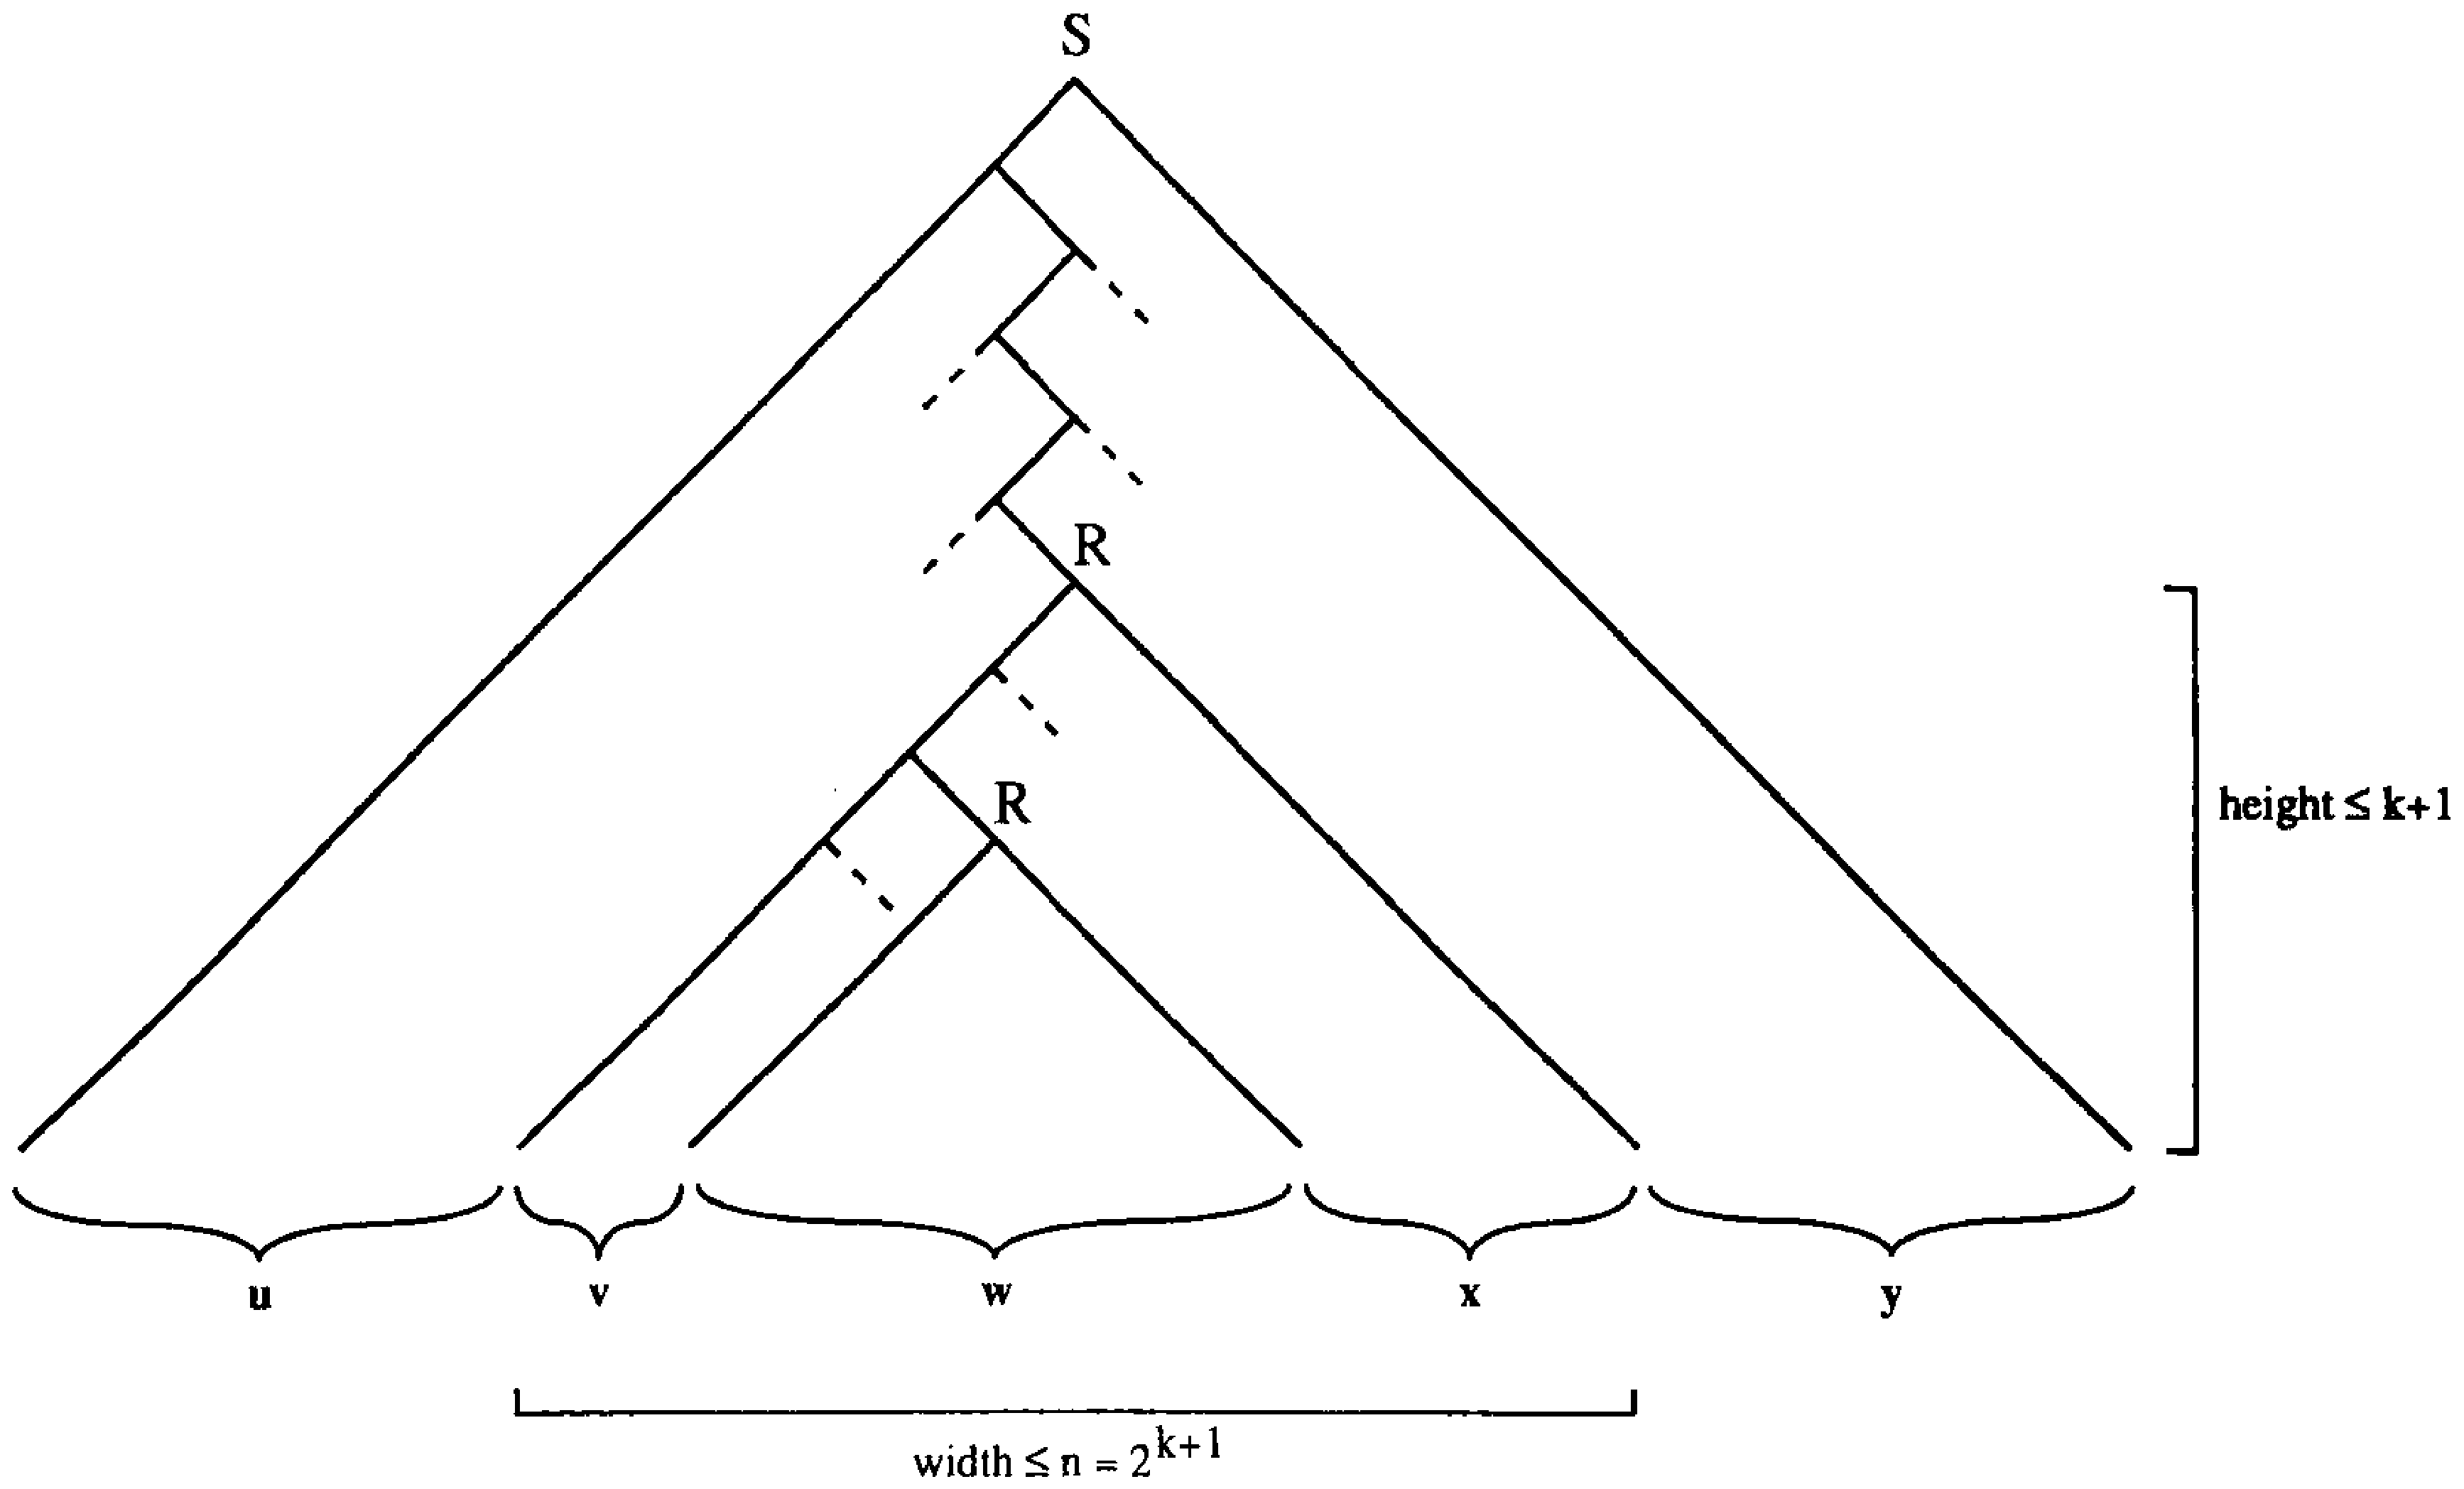
\epsfig{figure=ToFAfigures/fig9-12.eps,height=3.7in}}
\caption{The parse tree discussed in the proof of Theorem \ref{thm-9.7}}\label{fig-9.12}
\end{figure}

The two occurrences of R were in distinct places in the parse tree, and hence at
least one production was applied in deriving $uv\R xy$ from $u\R y$. Since the
PCNF grammar $G$ contains neither contracting productions nor unit productions,
the sentential form $uv\R xy$ must be of greater length than $u\R y$, and hence
$|v|+|x|>0$. Furthermore, the subtree rooted at the higher occurrence of R was
of height $k+1$ or less, and hence accounts for no more than $2^{k+1}(=n)$
terminals. Thus, $|vwx| \leq n$.\index{height of a parse tree}
All the criteria described in the pumping theorem are therefore met.

Since a
context-free language must be generated by a CNF grammar with a finite number of
nonterminals, there must exist a constant $n$ (such as $n = 2^{(\|\Omega\|+1)}$)
for which the existence of a string of length at least $n$ implies the existence
of an infinite sequence of distinct strings that must all belong to $L$, as
stated in the theorem.
\end{thm}

As with the pumping lemma, the pumping theorem is usually applied to justify
that certain languages are complex (by proving that the language does not
satisfy the pumping theorem and is thus not context free). Such proofs naturally
employ the contrapositive of Theorem \ref{thm-9.7}, which is stated next.

% Theorem 9.8
\begin{thm}\label{thm-9.8}
Let $L$ be a language over $\Sigma^*$. \\
{\bf if} $(\forall n\in\NN)(\exists z\in L \ni |z| \geq n)(\forall u,v,w,x,y \in
\Sigma^* \ni z = uvwxy, |vwx| \leq n, |vx|\geq 1)(\exists i\in\NN \ni uv^iwx^iy
\notin L)$ \\
{\bf then} $L$ is not context free.

\emph{Proof.} See the exercises.
\end{thm}

Examples 8.5 and 9.17 show that there are context-sensitive languages which are
not context free.

\subsection*{Example 9.17}

The language $L=\{a^kb^kc^k|\ k\in\NN\}$ is not a context-free language. Let $n$
be given, and choose $z=a^nb^nc^n$. Then $z\in L$ and $|z|= 3n \geq n$. If $L$
were context free, there must be choices for $u,\ v,\ w,\ x$, and $y$ satisfying
the pumping theorem. Every possible choice of these strings leads to a
contradiction, and hence $L$ cannot be context free. A sampling of the various
cases is outlined below.

If the strings $v$ and $x$ contain only one type of letter (for example, {\bf
c}), then $uv^2wx^2y$ will contain more $\pmb{c}$s than $\pmb{a}$s or $\pmb{b}$s, and
thus $uv^2wx^2y \notin L$. If $v$ were, say, all $\pmb{b}$s and $x$ were all {\bf
c}s, then $uv^2wx^2y$ would contain too few $\pmb{a}$s and would again not be a
member of $L$. If $v$ were to contain two types of letters such as $v =
\pmb{aabb}$, then $uv^2wx^2y = uvvwxxy = u\pmb{aabbaabb}wxxy$ and would
represent a string that had some $\pmb{b}$s preceding some $\pmb{a}$s, and again
$uv^2wx^2y \notin L$. All other cases are similar to these, and they
collectively imply that $L$ is not a context-free language.
[The shortest choice for $vwx$ that can successfully be pumped is
$\pmb{ab}^n\pmb{c}$, but this violates the condition that $|vwx| \leq n$.]

Example 9.17 illustrates one major inconvenience of the pumping theorem: the
inability to specify which portion of the string is to be ``pumped.'' With the
pumping lemma in Chapter \ref{ch-2}, variants were explored that allowed the first $n$
letters to be pumped or the last $n$ letters to be pumped. Indeed, any $n$
consecutive letters in a word from an FAD language can be pumped. For
context-free languages, such precision is more elusive. The uncertainty as to
where the $vwx$ portion of the string was in Example 9.17 led to many subcases,
since all combinations of $u,\ v,\ w,\ x$, and $y$ had to be shown to lead to
contradictions. The following result, a variant of Ogden's lemma, allows some
choice in the placement of the portion of the string to be pumped in a ``long''
word from a context-free language.

% Theorem 9.9
\begin{thm}\label{thm-9.9}
Let $L$ be a context-free language over $\Sigma^*$. Then \\
$(\exists n\in\NN)$ \\
$(\forall z \in L \ni |z| \geq n$ and $z$ has any $n$ or more positions marked
as distinguished) \\
$(\exists u,v,w,x,y \in\Sigma^*) \ni z = uvwxy$, \\
$vwx$ contains no more than $n$ distinguished positions, \\
$vx$ contains at least one distinguished position, \\
$w$ contains at least one distinguished position, and \\
$(\forall i \in\NN)(uv^iwx^iy \in L)$

\emph{Proof.} Given a context-free language $L$, there must exist a PCNF grammar
$G=\langle\Omega,\Sigma,S,P\rangle$ generating $L - \{\lambda\}$. Let $n =
2^{\|\Omega\|+1}$. The proof is similar to that given for the pumping theorem
(Theorem \ref{thm-9.7}); the method for choosing the path now depends on the placement of
the distinguished positions. A suitable path is constructed by beginning at the
root of the binary parse tree and, at each level, descending to the right or
left to lengthen the path. The decision to go right or left is determined by
observing the number of distinguished positions generated in the right subtree
and the number of distinguished positions generated in the left subtree. The
path should descend into the subtree that has the larger number of distinguished
positions; ties can be broken arbitrarily. The resulting path will terminate at
a leaf corresponding to a distinguished position, will be of sufficient length
to guarantee a repeated label R within the bottom $\|\Omega\| + 1$ interior
nodes, and so on. The conclusions now follow in much the same manner as those
given in the pumping theorem.
\end{thm}

\subsection*{Example 9.18}

For the language $L=\{\pmb{a}^k\pmb{b}^k\pmb{c}^k|k \in\NN\}$ investigated in
Example 9.17, Ogden's lemma could be applied with the first $n$ letters of
$\pmb{a}^n\pmb{b}^n\pmb{c}^n$ as the distinguished positions. Since $w$ must
have at least one distinguished letter (that is, an $\pmb{a}$), and $u$ and $v$
must precede $w$, the $u$ and $v$ portions of the string would then be required
to be all $\pmb{a}$s. This greatly reduces the number of cases that must be
considered. Note that more than $n$ letters can be chosen as the distinguished
positions, and they need not be consecutive.

\section{Closure Properties}\label{9.5}

Recall that \CSIG\ represented the class of context-free languages over $\Sigma$.
The applications of the pumping theorem show that not every language is context
free. The ability to show that specific languages are not context free makes it
feasible to decide which language operators preserve context-free languages. The
context-free languages are closed under most of the operators considered in
Chapter \ref{ch-5}; the major exceptions are complement and intersection. We begin with a
definition of substitution for context-free languages.

% Definition 9.11
\begin{dfn}\label{dfn-9.11}
Let $\Sigma=\{\pmb{a}_1,\pmb{a}_2,\ldots,\pmb{a}_m\}$ be an alphabet and let
$\Gamma$ be a second alphabet. Given context-free languages $L_1,L_2,\ldots,L_m$
over $\Gamma$, define a \emph{\Index{substitution}} $s$: $\Sigma\rightarrow\wp
(\Gamma^*)$ by $s(\pmb{a}_i) = L_i$ for each $i=1,2,\ldots,m$, which can be
extended to $\overline{s}$: $\Sigma^* \rightarrow \wp(\Gamma^*)$ by
\[ \overline{s}(\lambda) = \lambda \]
and
\[ (\forall\pmb{a}\in\Sigma)(\forall x\in\Sigma^*)(\overline{s}(\pmb{a}\cdot x)
	= s(\pmb{a})\cdot\overline{s}(x)) \]
$\overline{s}$ can be further extended to operate on a language $L\subseteq
\Sigma^*$ by defining $\overline{s}$: $\wp(\Sigma^*)\rightarrow\wp(\Gamma^*)$,
where
\[ \overline{s}(L) = \bigcup\limits_{z\in L} \overline{s}(z) \]
\end{dfn}

A substitution is similar to a language homomorphism (Definition \ref{dfn-5.8}), where
letters were replaced by single words, and to the regular set substitution given
by Definition \ref{dfn-6.5}. For context-free languages, substitution denotes the
consistent replacement of the individual letters within each word of a
context-free language with sets of words. Each such set of words must also be a
context-free language, although not necessarily over the original alphabet.

\subsection*{Example 9.19}

Let $L=L(G_t)$, where
\[ G_t = \langle\{T\},\{\pmb{a},\pmb{b},\pmb{c},\pmb{d},\pmb{-}\},T,\{T
	\rightarrow\pmb{a}|\pmb{b}|\pmb{c}|\pmb{d}|T\pmb{-}T\}\rangle \]
\begin{center}\begin{tabular}{l}
Let $L_1$ denote the set of all valid FORTRAN identifiers. \\
Let $L_2$ denote the set of all strings denoting integer constants. \\
Let $L_3$ denote the set of all strings denoting real constants. \\
Let $L_4$ denote the set of all strings denoting double-precision constants. \\
\end{tabular}\end{center}
If the substitution $s$ were defined by $s(\pmb{a})=L_1,\ s(\pmb{b})=L_2,\ s(
\pmb{c})=L_3,\ s(\pmb{d})=L_4$, then $\overline{s}(L)$ would represent the set
of all unparenthesized FORTRAN expressions involving only the subtraction
operator.

In this example, $\overline{s}(L)$ is a language over a significant portion of
the ASCII alphabet, whereas the original alphabet consisted of only five symbols.
The result is still context free, and this can be proved for all substitutions
of context-free languages into context-free languages. In Example 9.19, the
languages $L_1$, through $L_4$ were not only context free, but were in fact
regular. There are clearly context-free grammars defining each of them, and it
should be obvious how to modify $G_t$ to produce a grammar that generates
$\overline{s}(L)$. If $G_1=\langle\Omega_1,\Sigma_1,S_1,P_1\rangle$ is a grammar
generating $L_1$ [perhaps using the productions shown in Example 8.1], for example, then occurrences of a in the productions of $G_t$
should simply be replaced by the start symbol $S_1$ of $G_1$ and the productions
of $P_1$ added to the new grammar that will generate $\overline{s}(L)$. This is
essentially the technique used to justify Theorem \ref{thm-9.10}. The closure theorem is
stated for substitutions that do not modify the terminal alphabet, but it is
also true in general, as a trivial modification of the following proof would
show.

% Theorem 9.10
\begin{thm}\label{thm-9.10}\index{closure!under substitution}\index{substitution!context free}
Let $\Sigma$ be an alphabet, and let $s$: $\Sigma\rightarrow\Sigma^*$ be a
substitution. Then \CSIG\ is closed under $\overline{s}$.

\emph{Proof.} Let $\Sigma=\{\pmb{a}_1,\pmb{a}_2,\ldots,\pmb{a}_m\}$. If $L$ is a
context-free language, then there is a context-free grammar $G=\langle\Omega,
\Sigma,S,P\rangle$ that generates $L_1$. If $s$: $\Sigma\rightarrow\Sigma^*$ is
a substitution satisfying Definition \ref{dfn-9.11}, then for each letter $\pmb{a}_k\in
\Sigma$ there is a corresponding grammar $G_k=\langle\Omega_k,\Sigma_k,S_k,P_k
\rangle$ for which $L(G_k)=s(\pmb{a}_k)$. Since nonterminals can be freely
renamed, we may assume that $\Omega,\Omega_1,\Omega_2,\ldots,\Omega_m$ have no
common symbols. $\overline{s}(L)$ will be generated by the context-free grammar
\[ G' = \langle\Omega\cup\Omega_1\cup\Omega_2\cup\cdots\cup\Omega_m,\Sigma,S,P'
	\cup P_1\cup P_2\cup\cdots\cup P_m\rangle, \]
where $P'$ consists of the rules of $P$, with each appearance of $\pmb{a}_k$
replaced by $S_k$. From the start symbol $S$, the rules of $P'$ can be used as
they were in the original grammar $G$, producing strings with the start symbol
of the $k$th grammar where the $k$th terminal symbol would be. Since the
nonterminal sets were assumed to be pairwise disjoint, only the rules in $P_k$
can be used to expand $S_k$ resulting in the desired terminal strings from
$s(\pmb{a}_k)$. It follows that $L(G') = \overline{s}(L)$, and thus
$\overline{s}(L)$ is context free.
\end{thm}

% Theorem 9.11
\begin{thm}\label{thm-9.11}\index{closure!under language homomorphism}
Let $\Sigma$ be an alphabet, and let $\psi$: $\Sigma\rightarrow\Sigma^*$ be a
homomorphism. Then \CSIG\ is closed under \PBAR.

\emph{Proof.} Languages that consist of single words are obviously context free.
Hence, Theorem \ref{thm-9.10} applies when single words are substituted for letters. Since
homomorphisms are therefore special types of substitutions, \CSIG\ is closed
under homomorphism.
\end{thm}

Many of the other closure properties of the collection of context-free grammars
follow immediately from the result for substitution. Closure under union could
be proved by essentially the same method presented in Theorem \ref{thm-8.4}. An alternate
proof, based on Theorem \ref{thm-9.10}, is given next.

% Theorem 9.12
\begin{thm}\label{thm-9.12}\index{closure!under union}
Let $\Sigma$ be an alphabet, and let $L_1$ and $L_2$ be context-free languages
over $\Sigma$. Then $L_1\cup L_2$ is context free. Thus, \CSIG\ is closed under
union.

\emph{Proof.} Assume $L_1$ and $L_2$ are context-free languages over $\Sigma$.
The grammar \  $\cup =\langle\{S\},\{\pmb{a},\pmb{b}\},S,\{S\rightarrow\pmb{a},S
\rightarrow\pmb{b}\}\rangle$ clearly generates the context-free language
$\{\pmb{a},\pmb{b}\}$. The substitution defined by $s(\pmb{a})=L_1$ and $s(
\pmb{b})=L_2$ gives rise to the language $\overline{s}(\{\pmb{a},\pmb{b}\})$,
which obviously equals $L_1\cup L_2$. By Theorem \ref{thm-9.10}, this language must be
context free.
\end{thm}

A similar technique can be used for concatenation and Kleene closure. It is
relatively easy to directly construct appropriate new grammars that combine the
generative powers of the original grammars. The exercises explore constructions
that prove these closure properties without relying on Theorem \ref{thm-9.10}.

% Theorem 9.13
\begin{thm}\label{thm-9.13}\index{closure!under concatenation}
Let $\Sigma$ be an alphabet, and let $L_1$ and $L_2$ be context-free languages
over $\Sigma$. Then $L_1\cdot L_2$ is context free. Thus, \CSIG\ is closed under
concatenation.

\emph{Proof.} Let $L_1$ and $L_2$ be context-free languages over $\Sigma$. The
pure context-free grammar $C=\langle\{S\},\{\pmb{a},\pmb{b}\},\\S,\{S\rightarrow
\pmb{ab}\}\rangle$ generates the language $\{\pmb{ab}\}$. The substitution
defined by $s(\pmb{a})=L_1$ and $s(\pmb{b})=L_2$ gives rise to the language
$\overline{s}(\{\pmb{ab}\})=L_1\cdot L_2$. By Theorem \ref{thm-9.10}, $L_1\cdot L_2$ must
therefore be context free.
\end{thm}

Closure under Kleene closure could be justified by Theorem \ref{thm-9.10} in a similar
manner, since the context-free grammar
\[ K= \langle\{Z,S\},\{\pmb{a},\pmb{b}\},S,\{Z\rightarrow\lambda,Z\rightarrow S,
S\rightarrow\pmb{a}S,S\rightarrow\pmb{a}\}\rangle \]
generates the language $\pmb{a}^*$. The substitution defined by $s(\pmb{a})=L_1$
gives rise to the language $\overline{s}(\pmb{a}^*)$, which is $L^*_1$, and so
$L^*_1$ is also context free. The proof of Theorem \ref{thm-9.14} instead illustrates how
to modify an existing grammar.

% Theorem 9.14
\begin{thm}\label{thm-9.14}\index{closure!under Kleene closure}
Let $\Sigma$ be an alphabet, and let $L_1$ be a context-free language over
$\Sigma$. Then $L^*_1$ is context free. Thus, \CSIG\ is closed under Kleene
closure.

\emph{Proof.} If $L_1$ is a context-free language, then there is a pure
context-free grammar $G_1 = \langle\Omega_1,\Sigma,S_1,P_1\rangle$ that
generates $L_1 - \{\lambda\}$. Choose nonterminals $Z'$ and $S'$ such that $Z'
\notin\Omega_1$ and $S'\notin\Omega_1$, and define a new grammar
\[ G_* = \langle\Omega_1\cup\{S',Z'\},\Sigma,Z',P_1\cup\{Z'\rightarrow\lambda,Z'
	\rightarrow S',S'\rightarrow S'S_1,S'\rightarrow S_1\}\rangle \]
A straightforward induction shows that $L(G_*) = L(G_1)^*$.
\end{thm}

Thus, many of the closure properties of the familiar operators investigated in
Chapter \ref{ch-5} for regular languages carryover to the class of context-free
languages. Closure under intersection does not extend, as the next result shows.

% Lemma 9.3
\begin{lmm}\label{lmm-9.3}\index{closure!under intersection}
$\mathfrak{C}_{\{\pmb{a},\pmb{b},\pmb{c}\}}$ is \emph{not} closed under intersection.

\emph{Proof.} The languages $L_1=\{\pmb{a}^i\pmb{b}^j\pmb{c}^j|\ i,j\in\NN\}$ and
$L_2=\{\pmb{a}^n\pmb{b}^n\pmb{c}^m|\ n,m\in\NN\}$ are context free (see the
exercises), and yet $L_1 \cap L_2 = \{\pmb{a}^k\pmb{b}^k\pmb{c}^k|\ k\in\NN\}$ was
shown in Example 9.17 to be a language that was not context free. Hence
$\mathfrak{C}_{\{\pmb{a},\pmb{b}, \pmb{c}\}}$ is not closed under intersection.
\end{lmm}

The exercises show that \CSIG\ is not closed under intersection for any alphabet
$\Sigma$ with two or more letters. It was noted in Chapter \ref{ch-5} that De Morgan's laws
implied that any collection of languages that is closed under union and
complementation must also be closed under intersection. It therefore follows
immediately that $\mathfrak{C}_{\{\pmb{a},\pmb{b},\pmb{c}\}}$ cannot be closed
under complementation either.

% Lemma 9.4
\begin{lmm}\label{lmm-9.4}\index{closure!under complementation}
$\mathfrak{C}_{\{\pmb{a},\pmb{b},\pmb{c}\}}$ is \emph{not} closed under
complementation.

\emph{Proof.} Assume that $\mathfrak{C}_{\{\pmb{a},\pmb{b},\pmb{c}\}}$ is closed
under complementation. Then any two context-free languages $L_1$ and $L_2$ would
have context-free complements $\sim\!\!L_1$ and $\sim\!\!L_2$. By Theorem \ref{thm-9.12},
$\sim\!\!L_1\ \cup \sim\!\!L_2$ is context free, and the assumption would imply
that its complement is also context free. But $\sim\!\!(\sim\!\!L_1\ \cup\sim\!\!
L_2)=L_1\cap L_2$, which would contradict Lemma \ref{lmm-9.3} (for example, if $L_1$ were
$\{\pmb{a}^i\pmb{b}^j\pmb{c}^j|\ i,j\in\NN\}$ and $L_2$ were $\{\pmb{a}^n\pmb{b}^n
\pmb{c}^m|\ n,m\in\NN\}$). Hence the assumption must be false and $\mathfrak{C}_{
\{\pmb{a},\pmb{b},\pmb{c}\}}$ cannot be closed under complementation.
\end{lmm}

Thus, the context-free languages do not enjoy all of the closure properties that
the regular languages do. However, the distinction between a regular language
and a context-free language is lost if the underlying alphabet contains only one
letter, as shown by the following theorem. The proof demonstrates that there is
a certain regularity in the lengths of \emph{any} context-free language. It is
the relationships between the different letters in the words of a context-free
language that give it the potential for being non-FAD. If $L$ is a context-free
language over the singleton alphabet $\{\pmb{a}\}$, then no such complex
relationships can exist; the character of a word is determined solely by its
length.

% Theorem 9.15
\begin{thm}\label{thm-9.15}
$\mathfrak{C}_{\{\pmb{a}\}} = \mathfrak{D}_{\{\pmb{a}\}}$; that is, every
context-free language over a single-letter alphabet is regular.

\emph{Proof.} Let $L$ be a context-free language over the singleton alphabet
$\{\pmb{a}\}$, and assume the CNF grammar $G=\langle\Omega,\Sigma,S,P\rangle$
generates $L$. Let $n = 2^{\|\Omega\|+1}$. Consider the words in $L$ that are of
length $n$ or greater, choose the smallest such word, and denote it by
$\pmb{a}^{j_1}$. Since $j_1 \geq n$, the pumping theorem can be applied to this
word, and hence $\pmb{a}^{j_1}$ can be written as $uvwxy$, where $u=\pmb{a}^{p_1},\ 
v=\pmb{a}^{q_1},\ w=\pmb{a}^{r_1},\ x=\pmb{a}^{s_1}$, and $y=\pmb{a}^{t_1}$. Let
$i_1=q_1+s_1$. Note that $|vwx|\leq n$ implies that $i_1 \leq n$. The pumping
theorem then implies that all strings in the set $L_1=\{\pmb{a}^{j_i+k_{i_1}}|k=0,1,
2,\ldots\}$ must belong to $L$. These account for many of the large words in $L$.
If there are other large words in $L$, choose the next smallest word $\pmb{a}^{
j_2}$ that is of length greater than $n$ that belongs to $L$ but is not already
in the set $L_1$. By a similar argument, there is an integer $i_2 \leq $n for
which all strings in the set $L_2=\{\pmb{a}^{j_2+k_{i_2}}|k=0,1,2,\ldots\}$ must also
belong to $L$. Note that if $i_1$ happens to equal $i_2$, then $j_1-j_2$ is not
a multiple of $n$, or else $\pmb{a}^{j_2}$ would belong to $L_1$. That is, $j_1$
and $j_2$ must in this case belong to different equivalence classes modulo $n$.
While large words remain unaccounted for, we continue choosing the next smallest
word $\pmb{a}^{j_{m+1}}$ that is of length greater than $n$ and belongs to $L$
but is not already in the set $L_1\cup L_2\cup\cdots\cup L_m$. Since each $i_k
\leq n$, there are at most $n$ choices for the $i_k$ values, and only $n$ different
equivalence classes mod $n$ in which the $j_k$ values may fall, totaling $n^2$
different combinations. Thus, all the long words in $L$ will be accounted for by
the time $m$ reaches $n^2$. The words in $L$ of length less than $n$ constitute
a finite set $F$, which is regular. Each $L_k$ is represented by the regular
expression indicated by $(\pmb{a}^{i_k})^*\cdot\pmb{a}^{j_k}$, and there are less
than $n^2$ of these expressions, so $L$ is the finite union of regular sets, and
is therefore regular.
\end{thm}

If a regular language is intersected with a context-free language, the result
may not be regular, but it will be context free. The proof that \CSIG\ is
closed under intersection with a regular set will use the tools developed in
Chapter \ref{ch-10}. The constructs in Chapter \ref{ch-10} will also allow us to show that \CSIG\ 
is closed under inverse homomorphism. Such results are useful in showing closure
under other operators and will also be useful in identifying certain languages
as non-context-free. These conclusions will be based on a more powerful type of
machine, called a pushdown automaton. The context-free languages will correspond
to the languages that can be represented by such recognizers.

\section*{Exercises}
\begin{enumerate}[{9.}1.]
\item Characterize the nature of parse trees of left-linear grammars.

\item Give context-free grammars for the following languages:
\begin{enumerate}
\item $\{\pmb{a}^n\pmb{b}^n\pmb{c}^m\pmb{d}^m|\ n,m\in\NN\}$
\item $\{\pmb{a}^i\pmb{b}^j\pmb{c}^j\pmb{d}^i|\ i,j\in\NN\}$
\item $\{\pmb{a}^n\pmb{b}^n\pmb{c}^m\pmb{d}^m|\ n,m\in\NN\}\cup\{\pmb{a}^i\pmb{b}^j
\pmb{c}^j\pmb{d}^i|\ i,j\in\NN\}$
\end{enumerate}

\item \begin{enumerate}
\item Find, if possible, unambiguous context-free grammars for each of the
languages given in Exercise 9.2.
\item Prove or disprove: If $L_1$ and $L_2$ are unambiguous context-free
languages, then $L_1 \cup L_2$ is also an unambiguous context-free language.
\item Is \USIG\ closed under union?
\end{enumerate}

\item State and prove the inductive result needed in Theorem \ref{thm-9.2}.

\item Consider the proof of Theorem \ref{thm-9.4}. Let $G=\langle\Omega,\Sigma,S,P\rangle$
be a context-free grammar, with the production set divided up into $P^u$ and
$P^n$ (the set of unit productions and the set of nonunit productions,
respectively). Devise an automaton-based algorithm that correctly calculates
$B^u = \{C\ |\ B\ \DRightarrow C\}$ for each nonterminal $B$ found in $P^u$.

\item \begin{enumerate}
\item What is wrong with proving that \CSIG\ is closed under concatenation by
using the following construction? Let $G_1 = \langle\Omega_1,\Sigma,S_1,P_1
\rangle$ and $G_2 = \langle\Omega_2,\Sigma,S_2,P_2\rangle$ be two context-free
grammars, and without loss of generality assume that $\Omega_1\cap\Omega_2 =
\emptyset$. Choose a new nonterminal $Z$ such that $Z\notin\Omega_1\cup\Omega_2$,
and define a new grammar $G^* = \langle\Omega_1\cup\Omega_2\cup\{Z\},\Sigma,Z,
P_1\cup P_2\cup\{Z\rightarrow S_1\cdot S_2\}\rangle$. \emph{Note:} It is
straightforward to show that $L(G^*) = L(G_1)\cdot L(G_2)$.
\item Modify $G^*$ so that it reflects an appropriate valid context-free
grammar. (\emph{Hint:} Pay careful attention to the treatment of lambda
productions.)
\item Prove that \CSIG\ is closed under concatenation by using the construction
defined in part (b).
\end{enumerate}

\item Let $\Sigma=\{\pmb{a},\pmb{b},\pmb{c}\}$. Show that $\{\pmb{a}^i\pmb{b}^j
\pmb{c}^k|\ i,j,k\in\NN$ and $i+j=k\}$ is context free.

\item \begin{enumerate}
\item Show that the following right-linear grammar is ambiguous.
\[ G=\langle\{S,A,B\},\{\pmb{a}\},S,\{S\rightarrow A,S\rightarrow B,A\rightarrow
\pmb{aa}A,A\rightarrow \lambda,B\rightarrow\pmb{aaa}B,B\rightarrow \lambda\}\rangle \]
\item Use the method outlined in Theorem \ref{thm-9.2} to remove the ambiguity in $G$.
\end{enumerate}

\item The regular expression grammar discussed in Example 9.3 produces strings
with needless outermost parentheses, such as $\pmb{((a\cup b)\cdot c)}$.
\begin{enumerate}
\item Define a grammar that generates all the words in this language and strings
that are stripped of (only) the outermost parentheses, as in $\pmb{(a\cup b)
\cdot c}$.
\item Define a grammar that generates all the words in this language and also
allows extraneous sets of parentheses, such as $\pmb{((((a)\cup b))\cdot c)}$.
\end{enumerate}

\item For the regular expression grammar discussed in Example 9.3:
\begin{enumerate}
\item Determine the leftmost derivation for $\pmb{((a^*\cdot b)\cup(c\cdot d)^*)}$.
\item Determine the rightmost derivation for $\pmb{((a^*\cdot b)\cup(c\cdot d)^*)}$.
\end{enumerate}

\item Consider the grammars $G$ and $G'$ in the proof of Theorem \ref{thm-9.5}. Induct on
the number of steps in a derivation in $G$ to show that $L(G) = L(G')$.

\item For a grammar $G$ in Chomsky normal form, prove by induction that for any
string $x \in L(G)$ other than $x=\lambda$ the number of productions applied to
derive $x$ is $2|x|$.

\item \begin{enumerate}
\item For a grammar $G$ in Chomsky normal form and a string $x \in L(G)$, state
and prove a lower bound on the depth of the parse tree for $x$.
\item For a grammar $G$ in Chomsky normal form and a string $x \in L(G)$, state
and prove an upper bound on the depth of the parse tree for $x$.
\end{enumerate}

\item Convert the following grammars to Chomsky normal form.
\begin{enumerate}
\item $\langle\{S,B,C\},\{\pmb{a},\pmb{b},\pmb{c}\},S,\{S\rightarrow\pmb{a}B,S
\rightarrow\pmb{ab}C,B\rightarrow\pmb{bc},C\rightarrow\pmb{c}\}\rangle$
\item $\langle\{S,A,B\},\{\pmb{a},\pmb{b},\pmb{c}\},S,\{S\rightarrow\pmb{c}BA,S
\rightarrow B,A\rightarrow\pmb{c}B,A\rightarrow A\pmb{bb}S,B\rightarrow\pmb{aaa}
\}\rangle$
\item $\langle\{R\},\{\pmb{a},\pmb{b},\pmb{c},\pmb{(},\pmb{)},\pmb{\epsilon},
\pmb{\emptyset},\pmb{\cup},\pmb{\cdot},\pmb{^*}\},R,\{R\rightarrow\pmb{a}|\pmb{b}
|\pmb{c}|\pmb{\epsilon}|\pmb{\emptyset}|(R\pmb{\cdot}R)|(R\pmb{\cup}R)|R^{\pmb{*}
}\}\rangle$
\item $\langle\{T\},\{\pmb{a},\pmb{b},\pmb{c},\pmb{d},\pmb{-},\pmb{+}\},T,\{T
\rightarrow\pmb{a}|\pmb{b}|\pmb{c}|\pmb{d}|T\pmb{-}T|T\pmb{+}T\}\rangle$
\end{enumerate}

\item Convert the following grammars to Greibach normal form.
\begin{enumerate}
\item $\langle\{S_1,S_2\},\{\pmb{a},\pmb{b},\pmb{c},\pmb{d},\pmb{e}\},S_1,\{S_1
\rightarrow S_2S_1\pmb{e},S_1\rightarrow S_2\pmb{b},S_2\rightarrow S_1S_2,S_2
\rightarrow\pmb{c}\}\rangle$
\item $\langle\{S_1,S_2,S_3\},\{\pmb{a},\pmb{b},\pmb{c},\pmb{d},\pmb{e}\},S_1,
\{S_1\rightarrow S_3S_1, S_1\rightarrow S_2\pmb{a},S_2\rightarrow\pmb{be},S_3
\rightarrow S_2\pmb{c}\}\rangle$
\item $\langle\{S_1,S_2,S_3\},\{\pmb{a},\pmb{b},\pmb{c},\pmb{d},\pmb{e}\},S_1,
\{S_1\rightarrow S_1S_2\pmb{c},S_1\rightarrow\pmb{d}S_3,S_2\rightarrow S_1S_1,
S_2\rightarrow\pmb{a},S_3\rightarrow S_3\pmb{e}\}\rangle$
\end{enumerate}

\item Let $G$ be a context-free grammar, and obtain $G'$ from $G$ by adding
rules of the form $A\rightarrow\lambda$. Prove that there is a context-free
grammar $G''$ that is equivalent to $G'$. That is, show that apart from the
special rule $Z\rightarrow\lambda$ all other lambda productions are unnecessary.

\item Prove the following generalization of Lemma \ref{lmm-9.1}: Let $G=\langle\Omega,
\Sigma,S,P\rangle$ be a context-free grammar, and assume there are strings
$\alpha$ and $\gamma$ and nonterminals $X$ and $B$ for which $X\rightarrow\gamma
B\alpha\in P$. Further assume that the set of all $B$ rules is given by
$\{B\rightarrow\beta_1,B\rightarrow\beta_2,\ldots,B\rightarrow\beta_m\}$, and
let $G' = \langle\Omega,\Sigma,S,P'\rangle$, where
\[ P' = P\cup\{X_B\rightarrow\gamma\beta_1\alpha,X_B\rightarrow\gamma\beta_2
	\alpha,\ldots,X_B\rightarrow\gamma\beta_m\alpha\}-\{X\rightarrow\gamma
	B\alpha\}. \]
Then $L(G) = L(G')$.

\item Let $P=\{y\in\{\pmb{d}\}^*|\ \exists$ prime $p \ni y = \pmb{d}^P\}=\{\pmb{dd},
\pmb{ddd},\pmb{ddddd},\pmb{d}^7,\pmb{d}^{11},\pmb{d}^{13},\ldots\}$.
\begin{enumerate}
\item Prove that $P$ is not context free by directly applying the pumping
theorem.
\item Prove that $P$ is not context free by using the fact that $P$ is known to
be a nonregular language.
\end{enumerate}

\item Let $\Gamma=\{x\in\{\pmb{0},\pmb{1},\pmb{2}\}^*|\ \exists w\in\{\pmb{0},
\pmb{1}\}^* \ni x=w\cdot\pmb{2}\cdot w\}=\{\pmb{2},\pmb{121},\pmb{020},\pmb{1121
1},\pmb{10210},\ldots\}$. Prove that $\Gamma$ is not context free.

\item Let $\Psi=\{x\in\{\pmb{0},\pmb{1}\}^*|\ \exists w\in\{\pmb{0},\pmb{1}\}^*\ni
x = w\cdot w\}=\{\lambda,\pmb{00},\pmb{11},\pmb{0000},\pmb{1010},\pmb{1111},
\ldots\}$. Prove that $\Psi$ is not context free.

\item Let $\Xi=\{x\in\{\pmb{b}\}^*|\ \exists j\in\NN\ni |x|=2^j\}=\{\pmb{b},
\pmb{bb},\pmb{bbbb},\pmb{b}^8,\pmb{b}^{16},\pmb{b}^{32},\ldots\}$. Prove that
$\Xi$ is not context free.

\item Let $\Phi=\{x\in\{\pmb{a}\}^*|\ \exists j\in\NN \ni |x|= j^2\}=\{\lambda,
\pmb{a},\pmb{aaaa},\pmb{a}^9,\pmb{a}^{16},\pmb{a}^{25},\ldots\}$, and let
\[ \Phi'=\{x\in\{\pmb{b},\pmb{c},\pmb{d}\}^*|\ |x|_{\pmb{b}}\geq 1 \wedge |x|_{
	\pmb{c}}=(|x|_{\pmb{d}})^2\}. \]
\begin{enumerate}
\item Prove that $\Phi$ is not context free.
\item Use the conclusion of part (a) and the properties of homomorphism to prove
that $\Phi'$ is not context free.
\item Use Ogden's lemma to directly prove that $\Phi'$ is not context free.
\item Is it possible to use the pumping theorem to directly prove that $\Phi'$
is not context free?
\end{enumerate}

\item Consider $L=\{y\in\{\pmb{0},\pmb{1}\}^*|\ \ |y|_{\pmb{0}}=|y|_{\pmb{1}}\}$.
Prove or disprove that $L$ is context free.

\item Refer to the proof of Theorem \ref{thm-9.9}.
\begin{enumerate}
\item Give a formal recursive definition of the path by (1) stating boundary
conditions, and (2) giving a rule for choosing the next node on the path.
\item Show that the conclusions of Theorem \ref{thm-9.9} follow from the properties of
this path.
\end{enumerate}

\item Show that \CSIG\ is closed under $\cup$ by directly constructing a new
context-free grammar with the appropriate properties.

\item Let \XSIG\ be the set of all languages that are \emph{not} context free.\index{X@\XSIG \ (X-sigma )}
Determine whether or not:
\begin{enumerate}
\item \XSIG\ is closed under union.
\item \XSIG\ is closed under complement.
\item \XSIG\ is closed under intersection.
\item \XSIG\ is closed under Kleene closure.
\item \XSIG\ is closed under concatenation.
\end{enumerate}

\item Let $\Sigma$ be an alphabet, and $x=\pmb{a}_1\pmb{a}_2\cdots\pmb{a}_{n-1}
\pmb{a}_n\in\Sigma^*$; define $x^r=\pmb{a}_n\pmb{a}_{n-1}\cdots\pmb{a}_2\pmb{a}_1$.
For a language $L$ over $\Sigma$, define $L^r=\{x^r\ |\ x\in L\}$. Note that the
(unary) reversal operator $r$ is thus defined by $L^r=\{\pmb{a}_n\pmb{a}_{n-1}
\cdots\pmb{a}_3\pmb{a}_2\pmb{a}_1\ |\ \pmb{a}_1\pmb{a}_2\pmb{a}_3\cdots\pmb{a}_{n-1}
\pmb{a}_n\in L\}$, and $L^r$ therefore represents all the words in $L$ written
backward. Show that \CSIG\ is closed under the operator $r$.\index{closure!under reversal}

\item Let $\Sigma=\{\pmb{a},\pmb{b},\pmb{c},\pmb{d}\}$. Define the (unary)
operator T by
\begin{center}\begin{tabular}{r@{ = }l}
$T(L)$ & $\{\pmb{a}_n\pmb{a}_{n-1}\cdots\pmb{a}_3\pmb{a}_2\pmb{a}_1\pmb{a}_1
	\pmb{a}_2\pmb{a}_3\cdots\pmb{a}_{n-1}\pmb{a}_n|\pmb{a}_1\pmb{a}_2
	\pmb{a}_3\cdots\pmb{a}_{n-1}\pmb{a}_n\in L\}$ \\
& $\{w^r\cdot w|w\in L\}$
\end{tabular}\end{center}
(see the definition of $w^r$ in Exercise 9.27). Prove or disprove that \CSIG\ is
closed under the operator T.

\item Prove or disprove that $\mathfrak{C}_{\{\pmb{a},\pmb{b}\}}$ is closed
under \emph{relative complement}; that is, if $L_1$ and $L_2$ are context free,
then $L_1 - L_2$ is also context free.

\item \begin{enumerate}
\item Prove that $\mathfrak{C}_{\{\pmb{a},\pmb{b}\}}$ is not closed under
intersection, nor is it closed under complement.
\item By defining an appropriate homomorphism, argue that whenever $\Sigma$ has
more than one symbol, \CSIG\ is not closed under intersection, nor is it closed
under complement.
\end{enumerate}

\item Consider the iterative method discussed in the proof of Theorem \ref{thm-9.3}.
Outline an alternative method based on an automaton with states labeled by the
sets in $\wp(\Omega)$.

\item Consider grammars in Greibach normal form that also satisfy one of the
restrictions of Chomsky normal form; that is, no production has more than two
symbols on the right side.
\begin{enumerate}
\item Show that this is not a ``normal form'' for context-free languages by
demonstrating that there is a context-free language that cannot be generated by
any grammar in this form.
\item Characterize the languages generated by grammars that can be represented
by this restrictive form.
\end{enumerate}

\item Let $L$ be any collection of words over an alphabet $\Sigma$. Prove that
$L^*$ must be regular.

\item If $\|\Sigma\|=1$, prove or disprove that \CSIG\ is closed under
complementation.

\item Prove that $\{\pmb{a}^n\pmb{b}^n\pmb{c}^m|\ n,m\in\NN\}$ is context free.

\item Use Ogden's lemma to prove that $\{\pmb{a}^k\pmb{b}^n\pmb{c}^m|\ (k \not= n)
\wedge (n \not= m)\}$ is not context free.
\end{enumerate}
